\documentclass{article}
\usepackage[latin1]{inputenc}
\usepackage[T1]{fontenc}
\usepackage{ngerman}
\usepackage{graphicx}
\usepackage{pdfpages}
 
\title{Softwareprojekt:\\Kundenprojekt Web-Technologien II\\~\\Projektdokumentation\\ \small{- Team 4 -}}
\author{\underline{Team 4 besteht aus}:\\Damla Durmaz (bis zum 18.05.2012),\\HongLiang Jiang, Nicolas Lehmann,\\Tobias Schmid, Benjamin Sch\"onburg }
\date{\today}


\begin{document}

\renewcommand\abstractname{Worum geht es in diesem Softwareprojekt?}
\maketitle


%%%%%%%%%%%%%%%%%%% BESCHREIBUNG DES SWP %%%%%%%%%%%%%%%%%
\begin{abstract}
{\huge D}as Softwareprojekt Kundenprojekt Web-Technologien II simuliert ein reales, agiles Softwareprojekt in der freien Wirtschaft, im Speziellen im Unternehmen Carmeq in der Arbeitsgruppe Carmob. W\"ahrend des gesamten Softwareprojekts steht der Kunde im zentralen Fokus (Human Centered Design). Die Aufgabe der Teilnehmer dieses Softwareprojektes ist es eine Software zum Thema intermodales Reisen zu entwerfen und zu implementieren, die die Bed\"urfnisse der Mitarbeiter des Unternehmens Carmeq bez\"uglich deren durchgef\"uhrten Dienstreiseplanung und -durchf\"uhrung befriedigt. Die Projektarbeit umfasst die Bedarfsanalyse, die L\"osungsmodellierung, die Konzeptionierung der Software und der Implementierung dieser in einem agilen Prozess.\\
Anstatt eine Gesamtl\"osung zu entwerfen finden vier Softwareprojekte parallel zueinander statt, die jeweils einen anderen Teilaspekte als eigenst\"andiges Softwareprojekt umsetzen.\\
\\
Diese Projektdokumentation h\"alt den Verlauf der Arbeit von Team 4 fest. Diese Dokumentation ist nach Phasen und Wochen strukturiert und beschreibt die Aktivit\"aten des Teams w\"ahrend des Projekts, sowie auftretende Probleme und zentrale Entscheidungen und beschreibt zus\"atzlich die Ergebnisse jeder Phase der Projektarbeit.
\end{abstract}


%%%%%%%%%%%%%%%%%%% INHALTSVERZEICHNIS %%%%%%%%%%%%%%%%%%%

\newpage
\tableofcontents
\newpage


%%%%%%%%%%%%%%%%%%% INHALT %%%%%%%%%%%%%%%%%%%%%%%%%%%%%%%

\section{Phase: WarmUp}

Die WarmUp-Phase dient dazu sich gegenseitig kennenzulernen. Dieses gilt in Bezug auf das eigene Team, sowie auf den Kunden, die Mitarbeiter der Arbeitsgruppe Carmob der Carmeq GmbH. Die Organisation, die Idee des \textit{Human Centered Designs} und den agilen Charakter des Projekts kennenzulernen sind ebenfalls ein zentraler Bestandteil dieser Phase.

\subsection{Woche 01: Der Kunde und das Team, Interviews}

\subsubsection{Was hat das Team getan?}

Das Team hat sich kennen gelernt und dabei die St\"arken und Schw\"achen der Teammitglieder bestimmt und den ersten Kontakt zum Teamkunden hergestellt. Es wurde ein Projektordner auf \textit{GoogleDocs} erstellt und ein SVN-Repository erstellt um das kollaborative Arbeiten in den kommenden Wochen zu erm\"oglichen und zu organisieren. Jedes Teammitglied hat unabh\"angig von den anderen einen eigenen \textit{Leitfaden} entwickelt. Die Ergebnisse wurden im Teamtreffen zusammengef\"uhrt. Der dadurch entstandene \textit{Leitfaden} wurde in einem \textit{simulierten Kundengespr\"ach} strukturell getestet.

\subsubsection{Zentrale Entscheidungen}

Wir haben uns f\"ur \textit{GoogleDocs} als zentrale Arbeitsplattform entschieden, da diese das kollaborative Arbeiten erleichtert. Wir haben einen festen Termin f\"ur ein w\"ochentliches Teamtreffen organisert um den aktuellen Arbeitsstand austauschen und besser organisieren zu k\"onnen. Wir haben uns daf\"ur entschieden jedes Teammitglied einen verschiedenen Ansatz zu einem \textit{Leitfaden} entwickeln zu lassen, um somit auf eine m\"oglichst breit gef\"acherte Auswahl an Fragen zu kommen. Wir haben den konvergenten \textit{Leitfaden} getestet um die Zeit eventuell unerwartete Reaktionen ber\"ucksichtigen zu k\"onnen.

\subsection{Ergebnisse dieser Phase}

Wir haben aus den Vorschl\"agen der einzelnen Teammitglieder einen \textit{Interviewleitfaden} erstellt und diesen im Team in Form eines simulierten Kundeninterviews erfolgreich getestet.

\begin{itemize}
\item Interviewleitfaden (PDF)
\end{itemize}

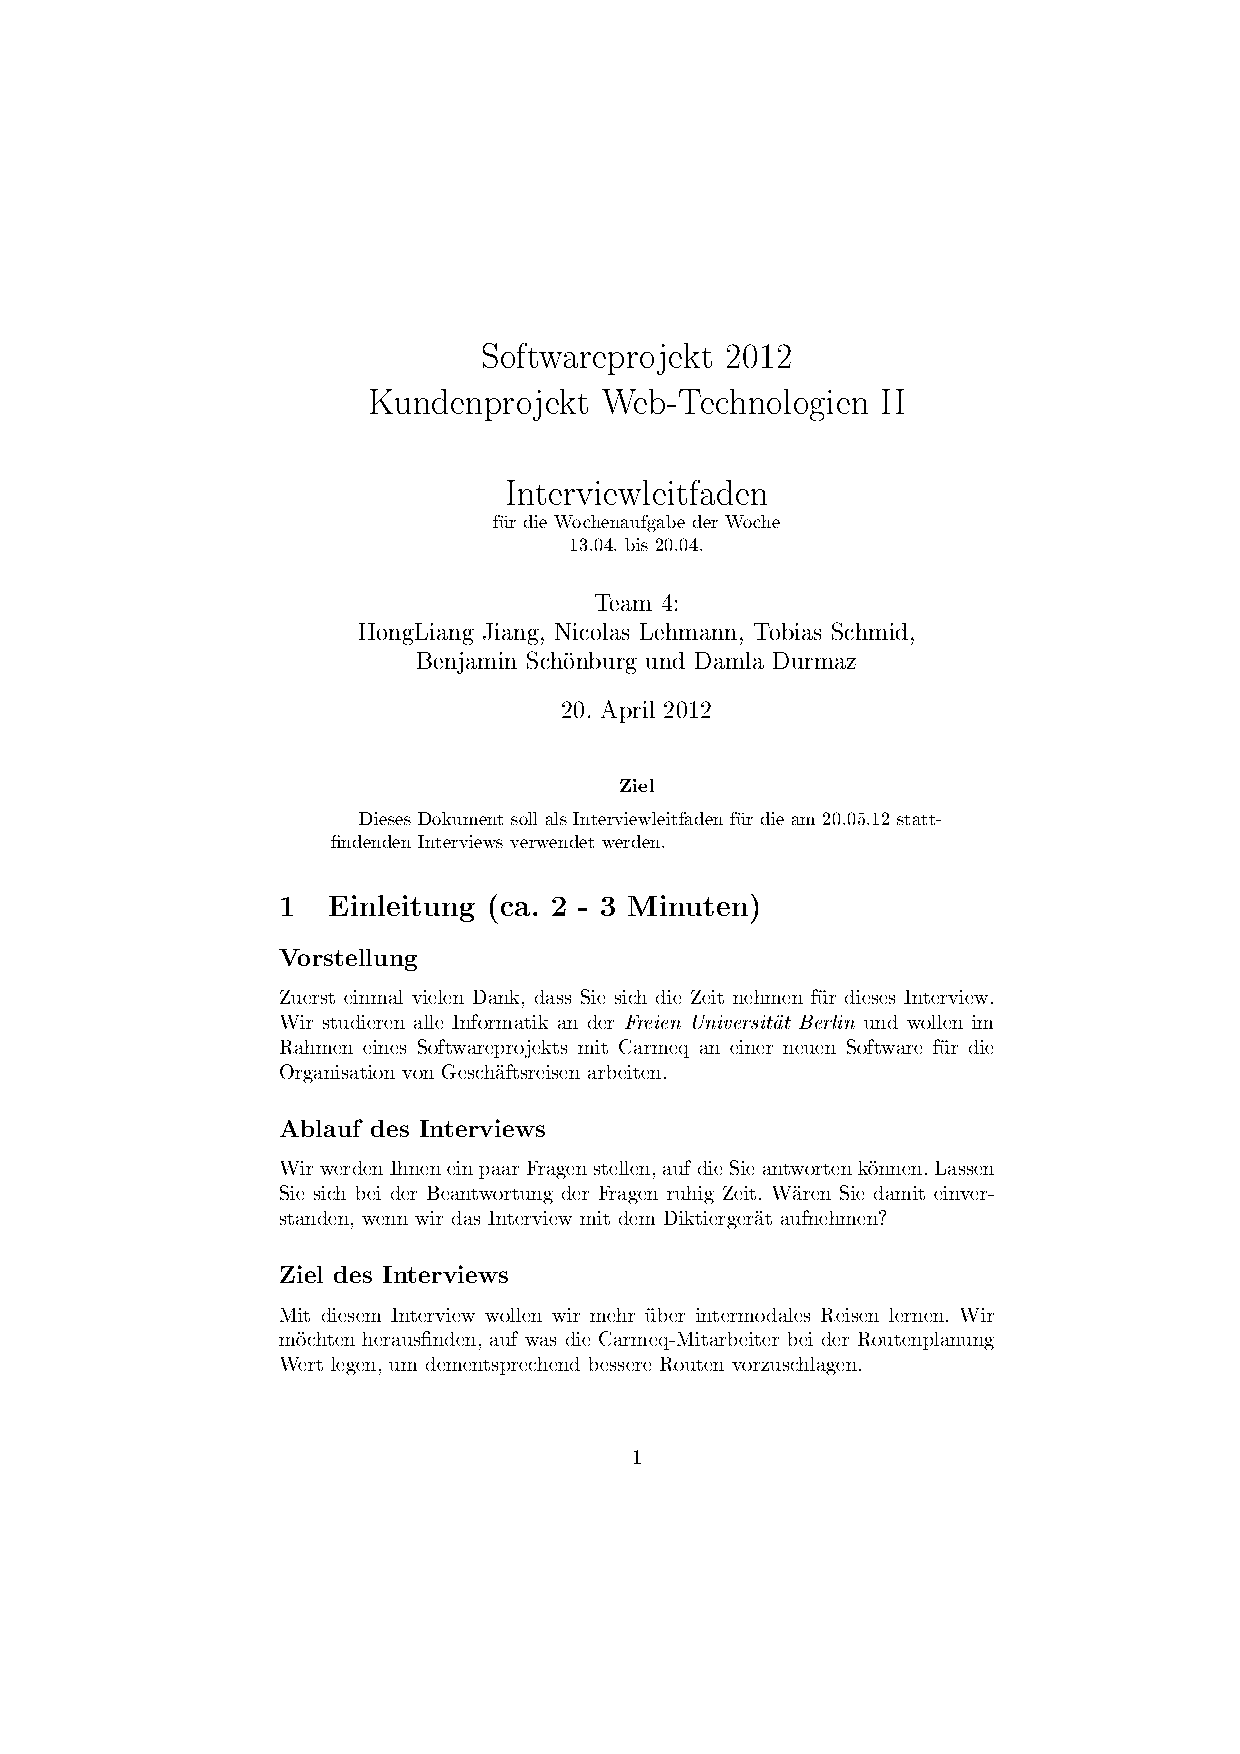
\includepdf[pages=1-4]{01_interviewleitfaden.pdf}

\section{Phase: Analyse, Modellierung und Konzeption}

Das Ziel diese Phase ist das Identifizieren der \textit{Nutzergruppen} und das Verstehen ihrer Bed\"urfnisse, im konkreten Fall die Mitarbeiter der Arbeitsgruppe Carmob der Carmeq GmbH. W\"ahrend dieser Phase wird die \textit{Nutzergruppe} in Form eines Interviews befragt und beobachtet um etwaiges Verhalten und bewusste, sowie unbewusste Bed\"urfnisse zu ermitteln oder abzuleiten, um innovative L\"osungen f\"ur die aufgedeckten Bedarfsfelder erzeugen zu k\"onnen. Im Zuge der Bedarfsermittlung wird mit den Methoden \textit{Story, Share \& Capture} und \textit{Clustering} gearbeitet um Informationen in der Gruppe zu synthetisieren damit ein gemeinsames Verst\"andins der Ist-Situation erreicht werden kann, aus der im Anschluss mit den Methoden \textit{Brainstorming} und \textit{Selektion} ein bedarfsgerechter L\"osungsansatz entwickelt werden kann. 

\subsection{Woche 02: Interviews, Nutzerkategorien, Persona, POV}

\subsubsection{Was hat das Team getan?}

Wir haben Interviews mit vier Mitarbeitern der Carmeq GmbH durchgef\"uhrt, diese analysiert und daraus \textit{Nutzerkategorien} abgeleitet. Wir haben uns daf\"ur entschieden sich jedes Teammitglied unabh\"angig von den anderen mit der Findung passender \textit{Nutzerkategorien} zu besch\"aftigen, um somit auf eine m\"oglichst gro\ss e Auswahl an Aspekten f\"ur potentielle \textit{Nutzerkategorien} zu kommen, die im Teamtreffen zusammengef\"uhrt wurden. Aus den identifizierten \textit{Nutzerkategorien} haben wir eine \textit{Persona} und einen \textit{POV} (Point of View) erstellt. Das Team hat die gesamte Problemstellung auf l\"osbare Problemstellungen eingeschr\"ankt.

\subsubsection{Zentrale Entscheidungen}

Bei der Ausarbeitung der \textit{Nutzerkategorien} haben wir uns auf eine relevante \textit{Nutzerkategorie} festgelegt: Der zeitsparenden Pendler. Wir haben die \textit{Persona} direkt aus der \textit{Nutzerkategorie} abgeleitet und diese durch m\"oglichst realisitsche, aber fiktive Daten erg\"anzt. Wir haben die Organisation und Durchf\"uhrung der Dienstreise, sowie die Nutzung der Reisezeit ins Zentrum gestellt.

\subsection{Woche 03: Konzeption}

\subsubsection{Was hat das Team getan?}

Wir haben drei konkrete Softwarel\"osungen entwickelt: \textit{ONE4ALL}, eine L\"osung, die ben\"otigte Dienste integriert und ein \textit{soziales Netzwerk} zur Organisation von Meetings w\"ahrend der Dienstreise mit der Deutschen Bahn, sowie eine L\"osung, die die \textit{Reisekostenabrechnung} vereinfacht. Wir haben aus unseren L\"osungen eine Pr\"asentation f\"ur die Kick-Off-Veranstaltung erstellt.

\subsubsection{Zentrale Entscheidungen}

Wir haben uns f\"ur die Abschlusspr\"asentation entschieden die beiden L\"osungen \textit{ONE4ALL} und das soziale Netzwerk zu integrieren und als eine Idee zu pr\"asentieren, da wir uns von dieser Idee am meisten Mehrwert versprochen haben. Die \textit{Reisekostenabrechnung} haben wir als alternative L\"osung mit aufgenommen. 

\subsection{Ergebnisse dieser Phase}

Wir haben die \textit{Interviews ausgewertet} und als Basis f\"ur die Erstellung von \textit{Nutzerkategorien} verwendet. Durch die Selektion von \textit{Nutzerkategorien} haben wir eine \textit{Persona} erstellt und diese zur Erstellung eines \textit{Point of Views} verwendet. Unser erster L\"osungsansatz war eine Kombination aus den Clustern \textit{Social Network} und \textit{ONE4ALL}. Diesen L\"osungsansatz haben wir trotz weiteren L\"osungsans\"atzen und seiner Mehrdimensionalit\"at favorisiert, wodurch er letztlich einer der zwei konkreten L\"osungen wurde, die wir f\"ur die \textit{Kick-Off-Pr\"asentation} ausgew\"ahlt haben. Wir haben eine \textit{Kick-Off-Pr\"asentation} erstellt, die zwei konkrete L\"osungen beinhaltete.

\begin{itemize}
\item Interviewauswertungen (PDF)
\item Nutzerkategorien (PDF)
\item Persona (PDF)
\item Point Of View (PDF)
\item Softwarel\"osung (JPG)
\item Kick-Off-Pr\"asentation (PDF)
\end{itemize}

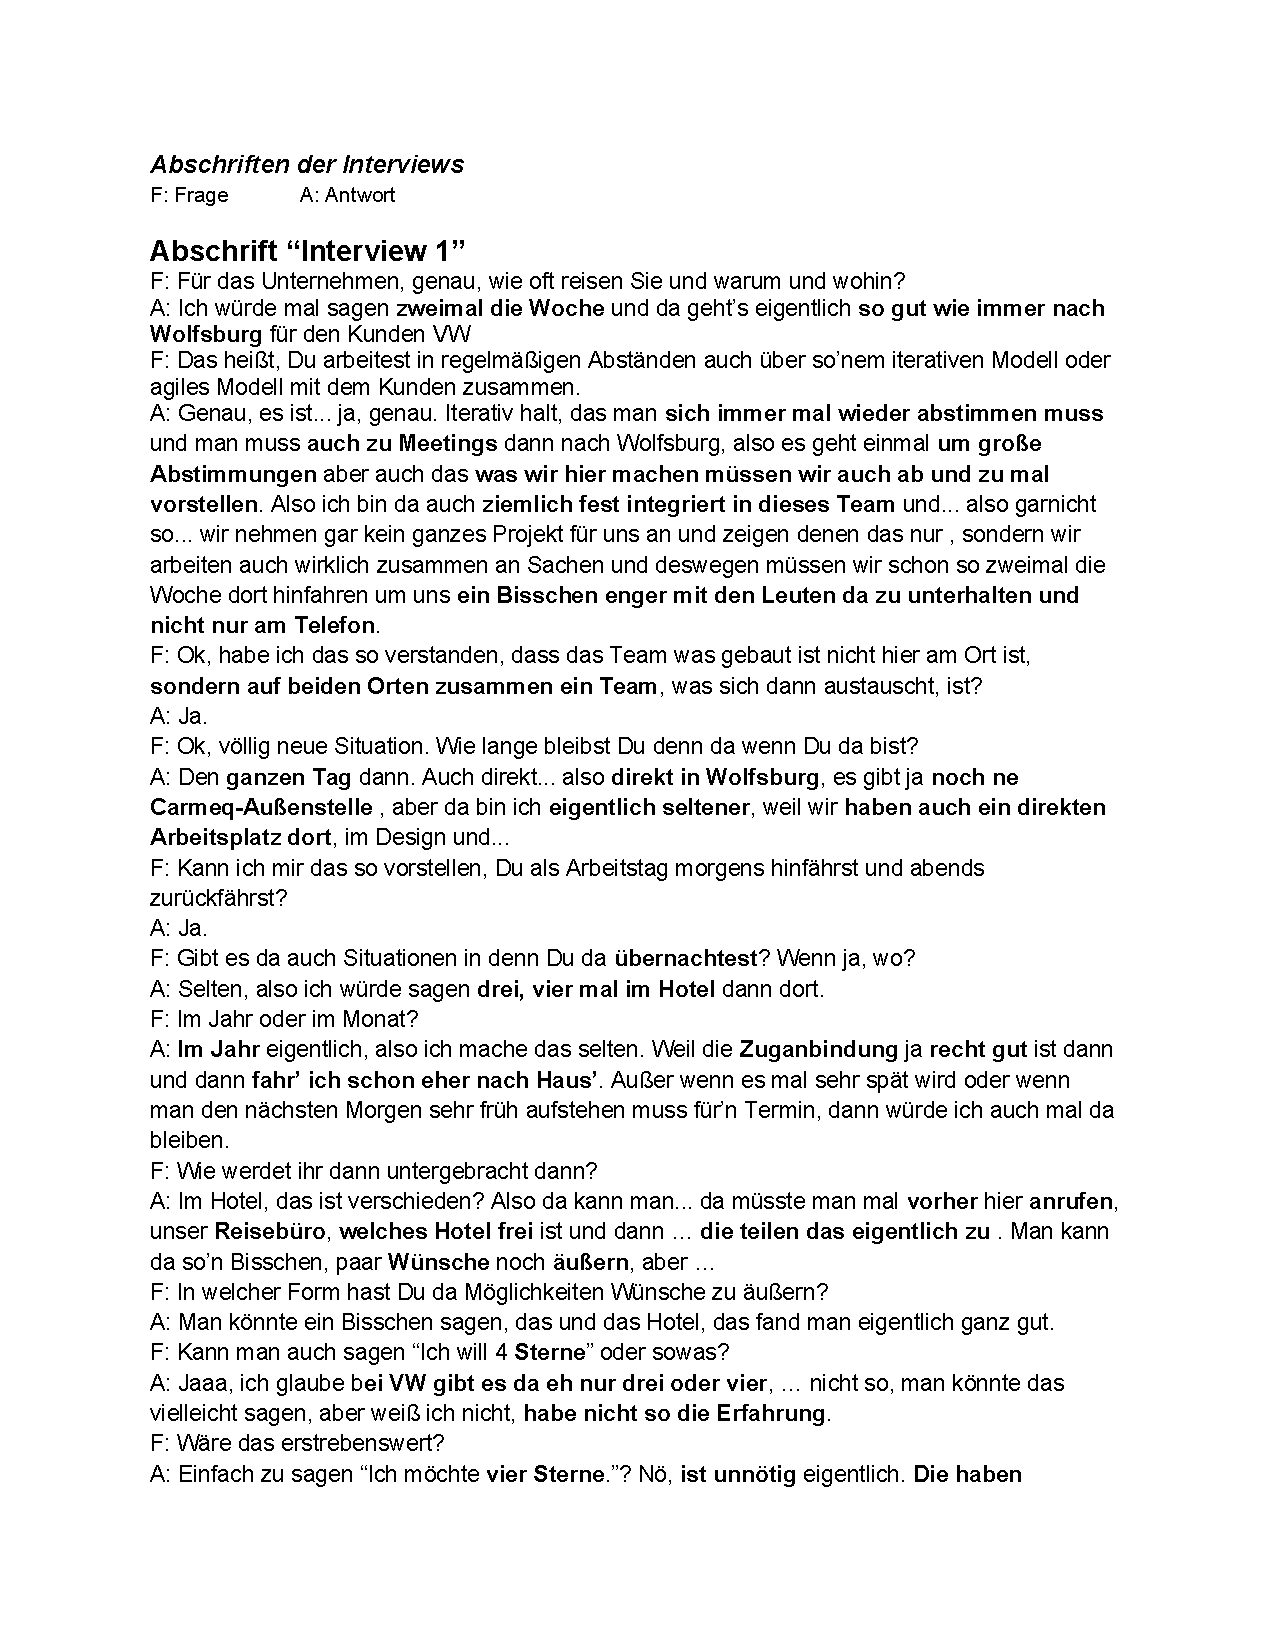
\includepdf[pages=1-12]{02_interviews_abschriften.pdf}
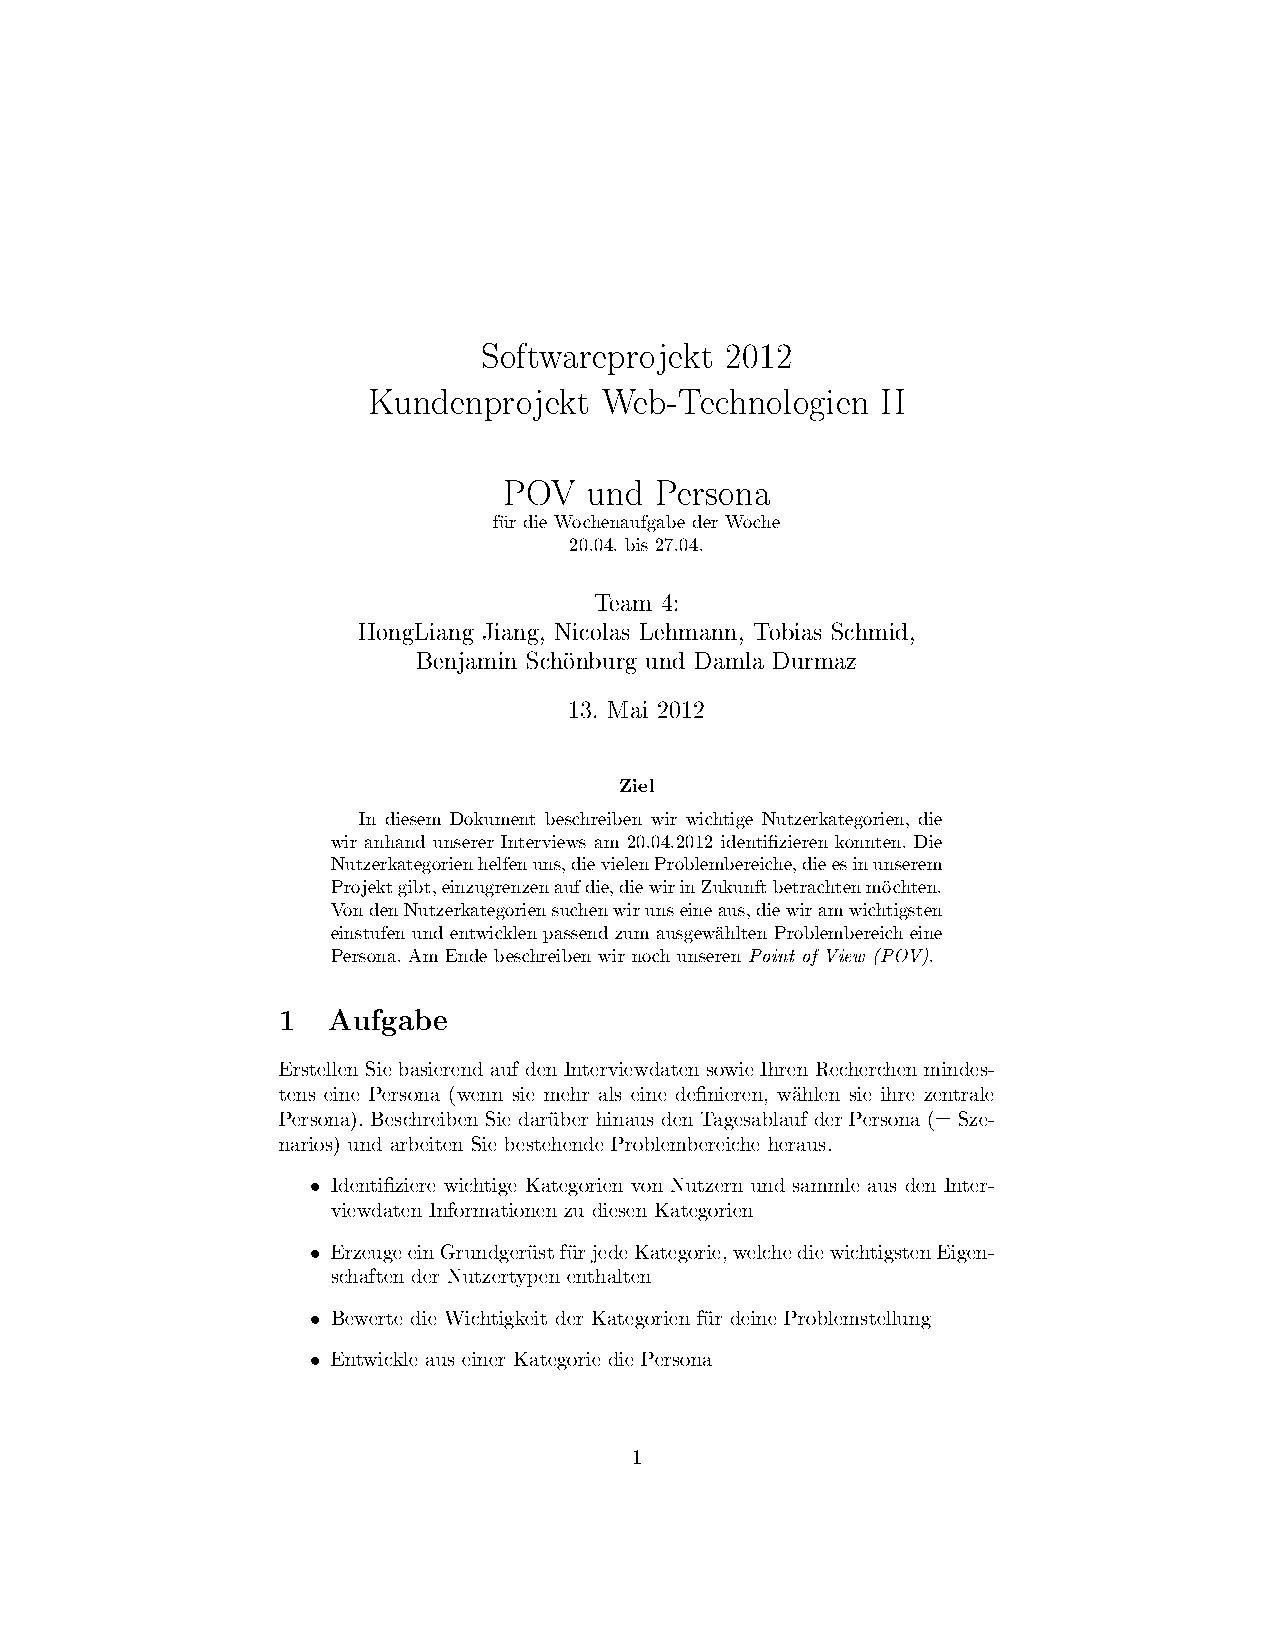
\includepdf[pages=1-9]{03_nutzerkategorien_persona_pov.pdf}
\begin{center}
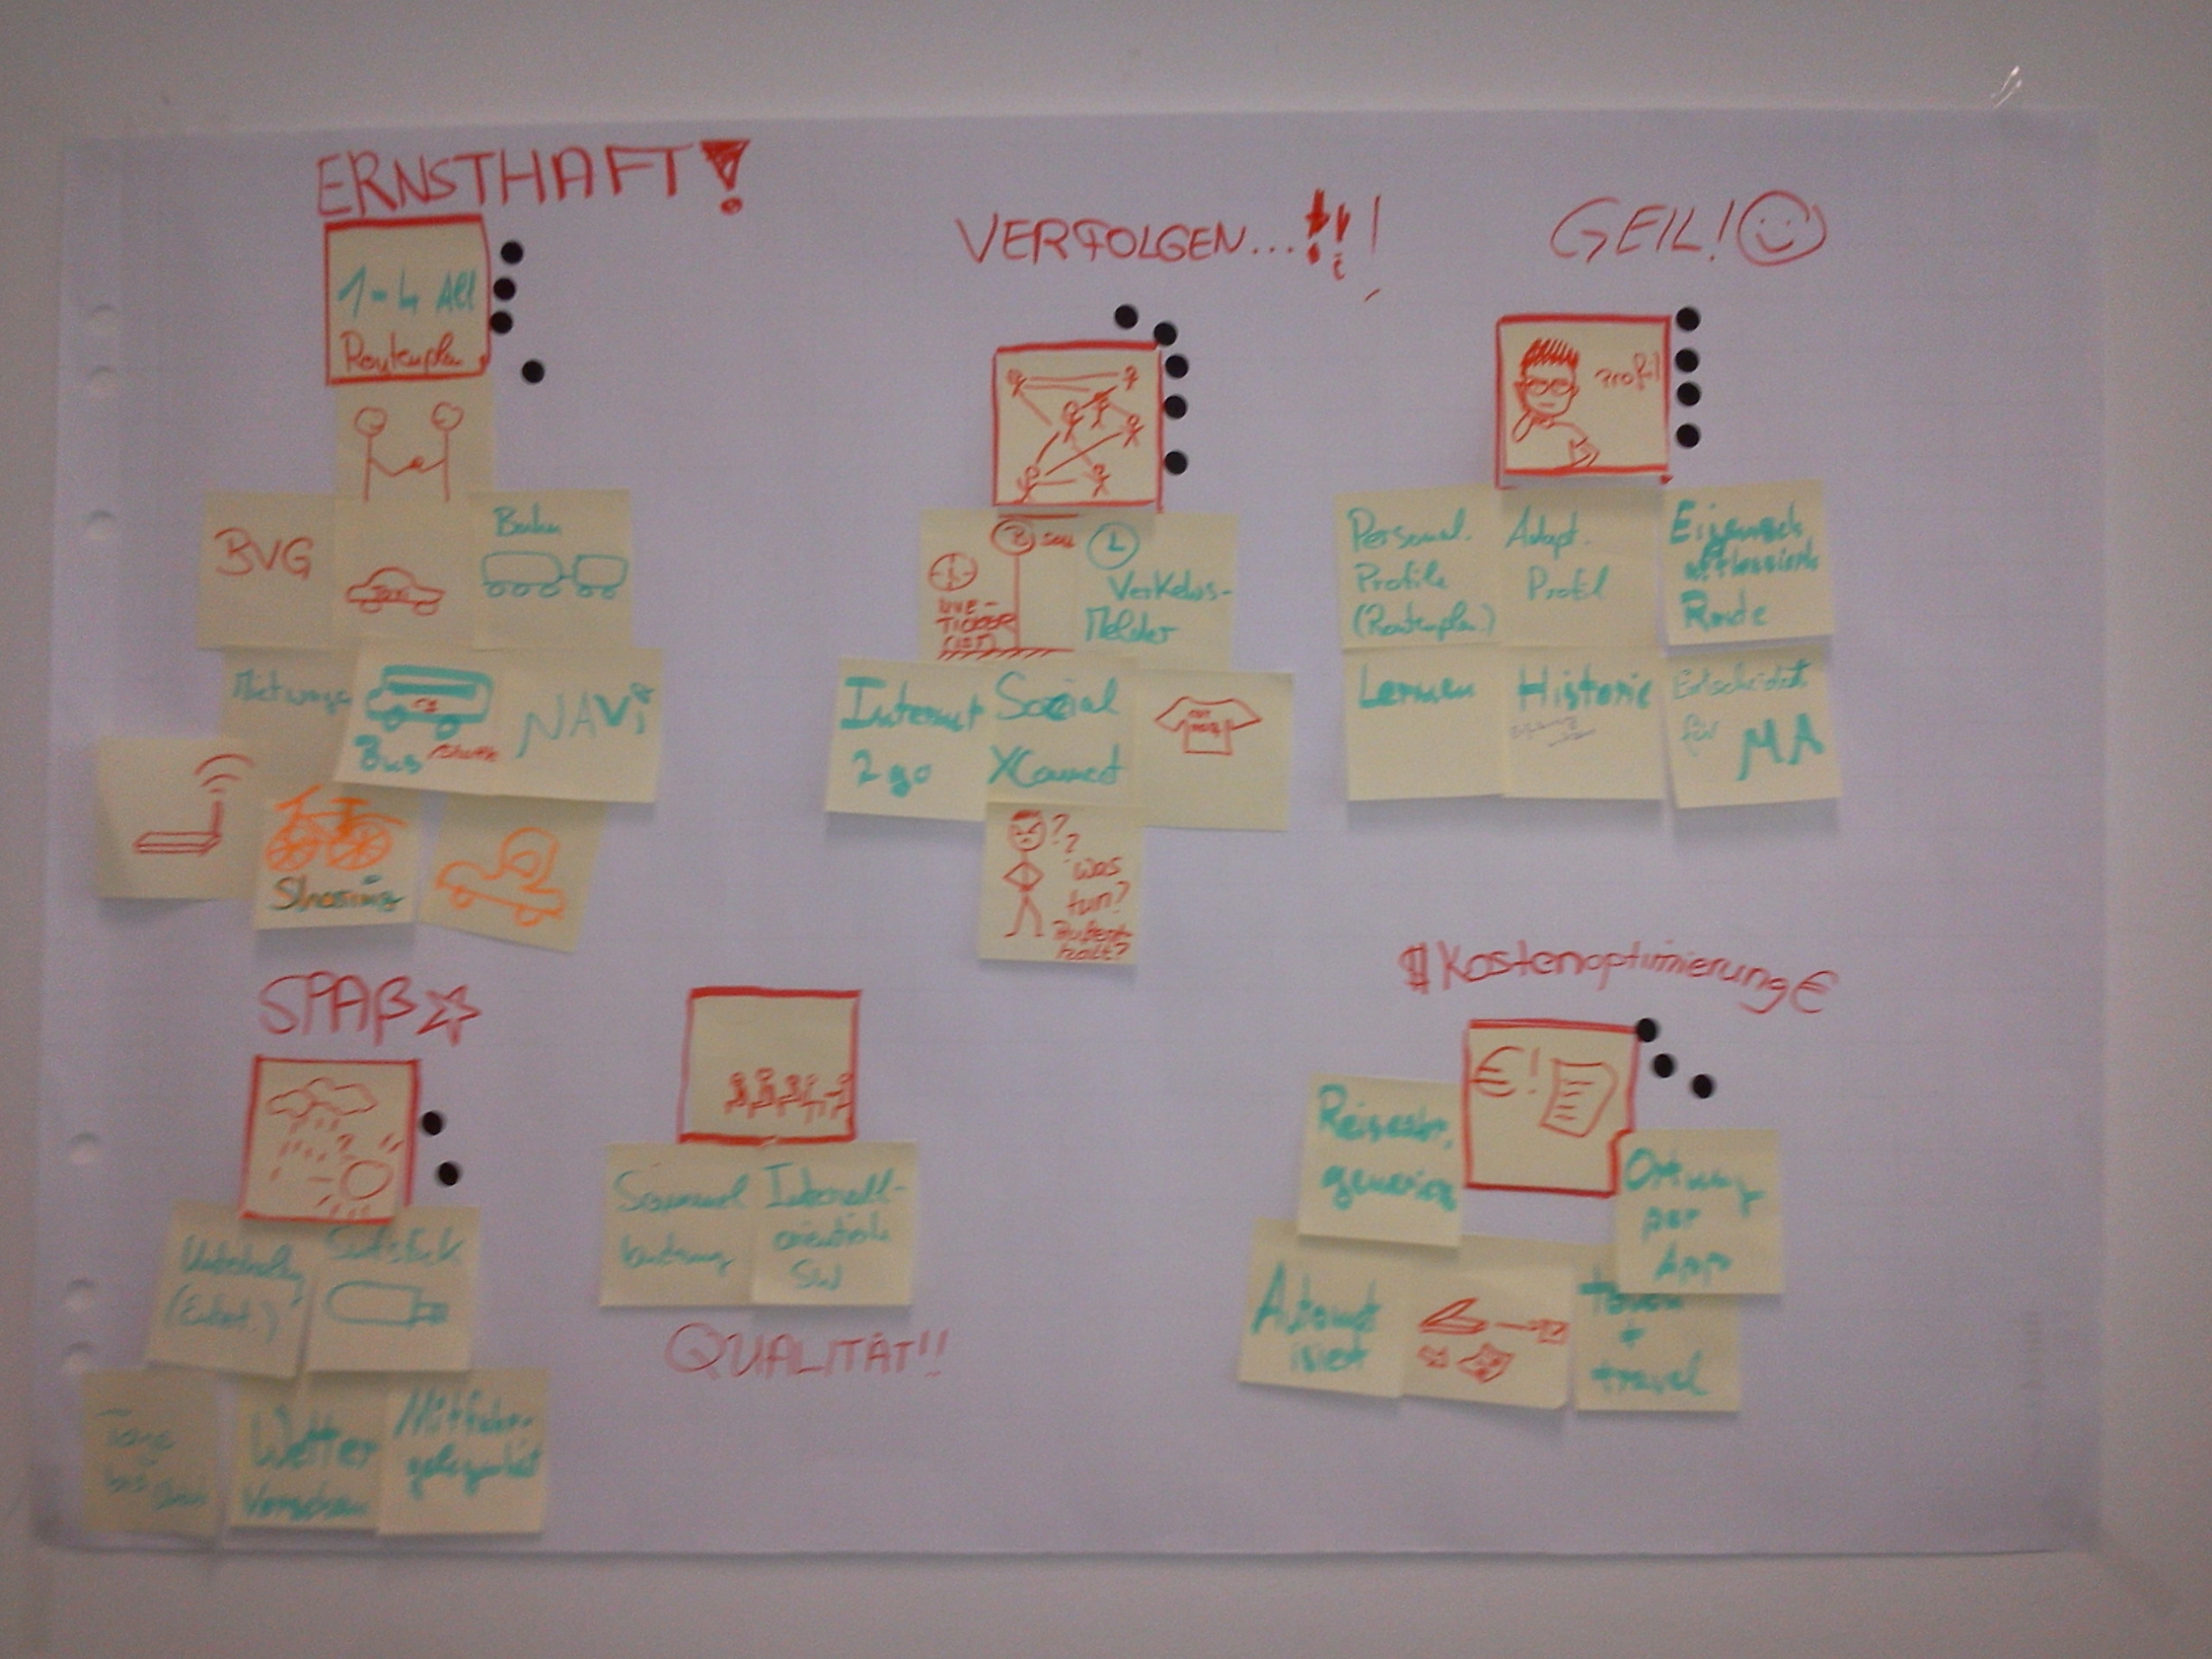
\includegraphics[width=12cm]{04_softwareloesung01.jpg}\\
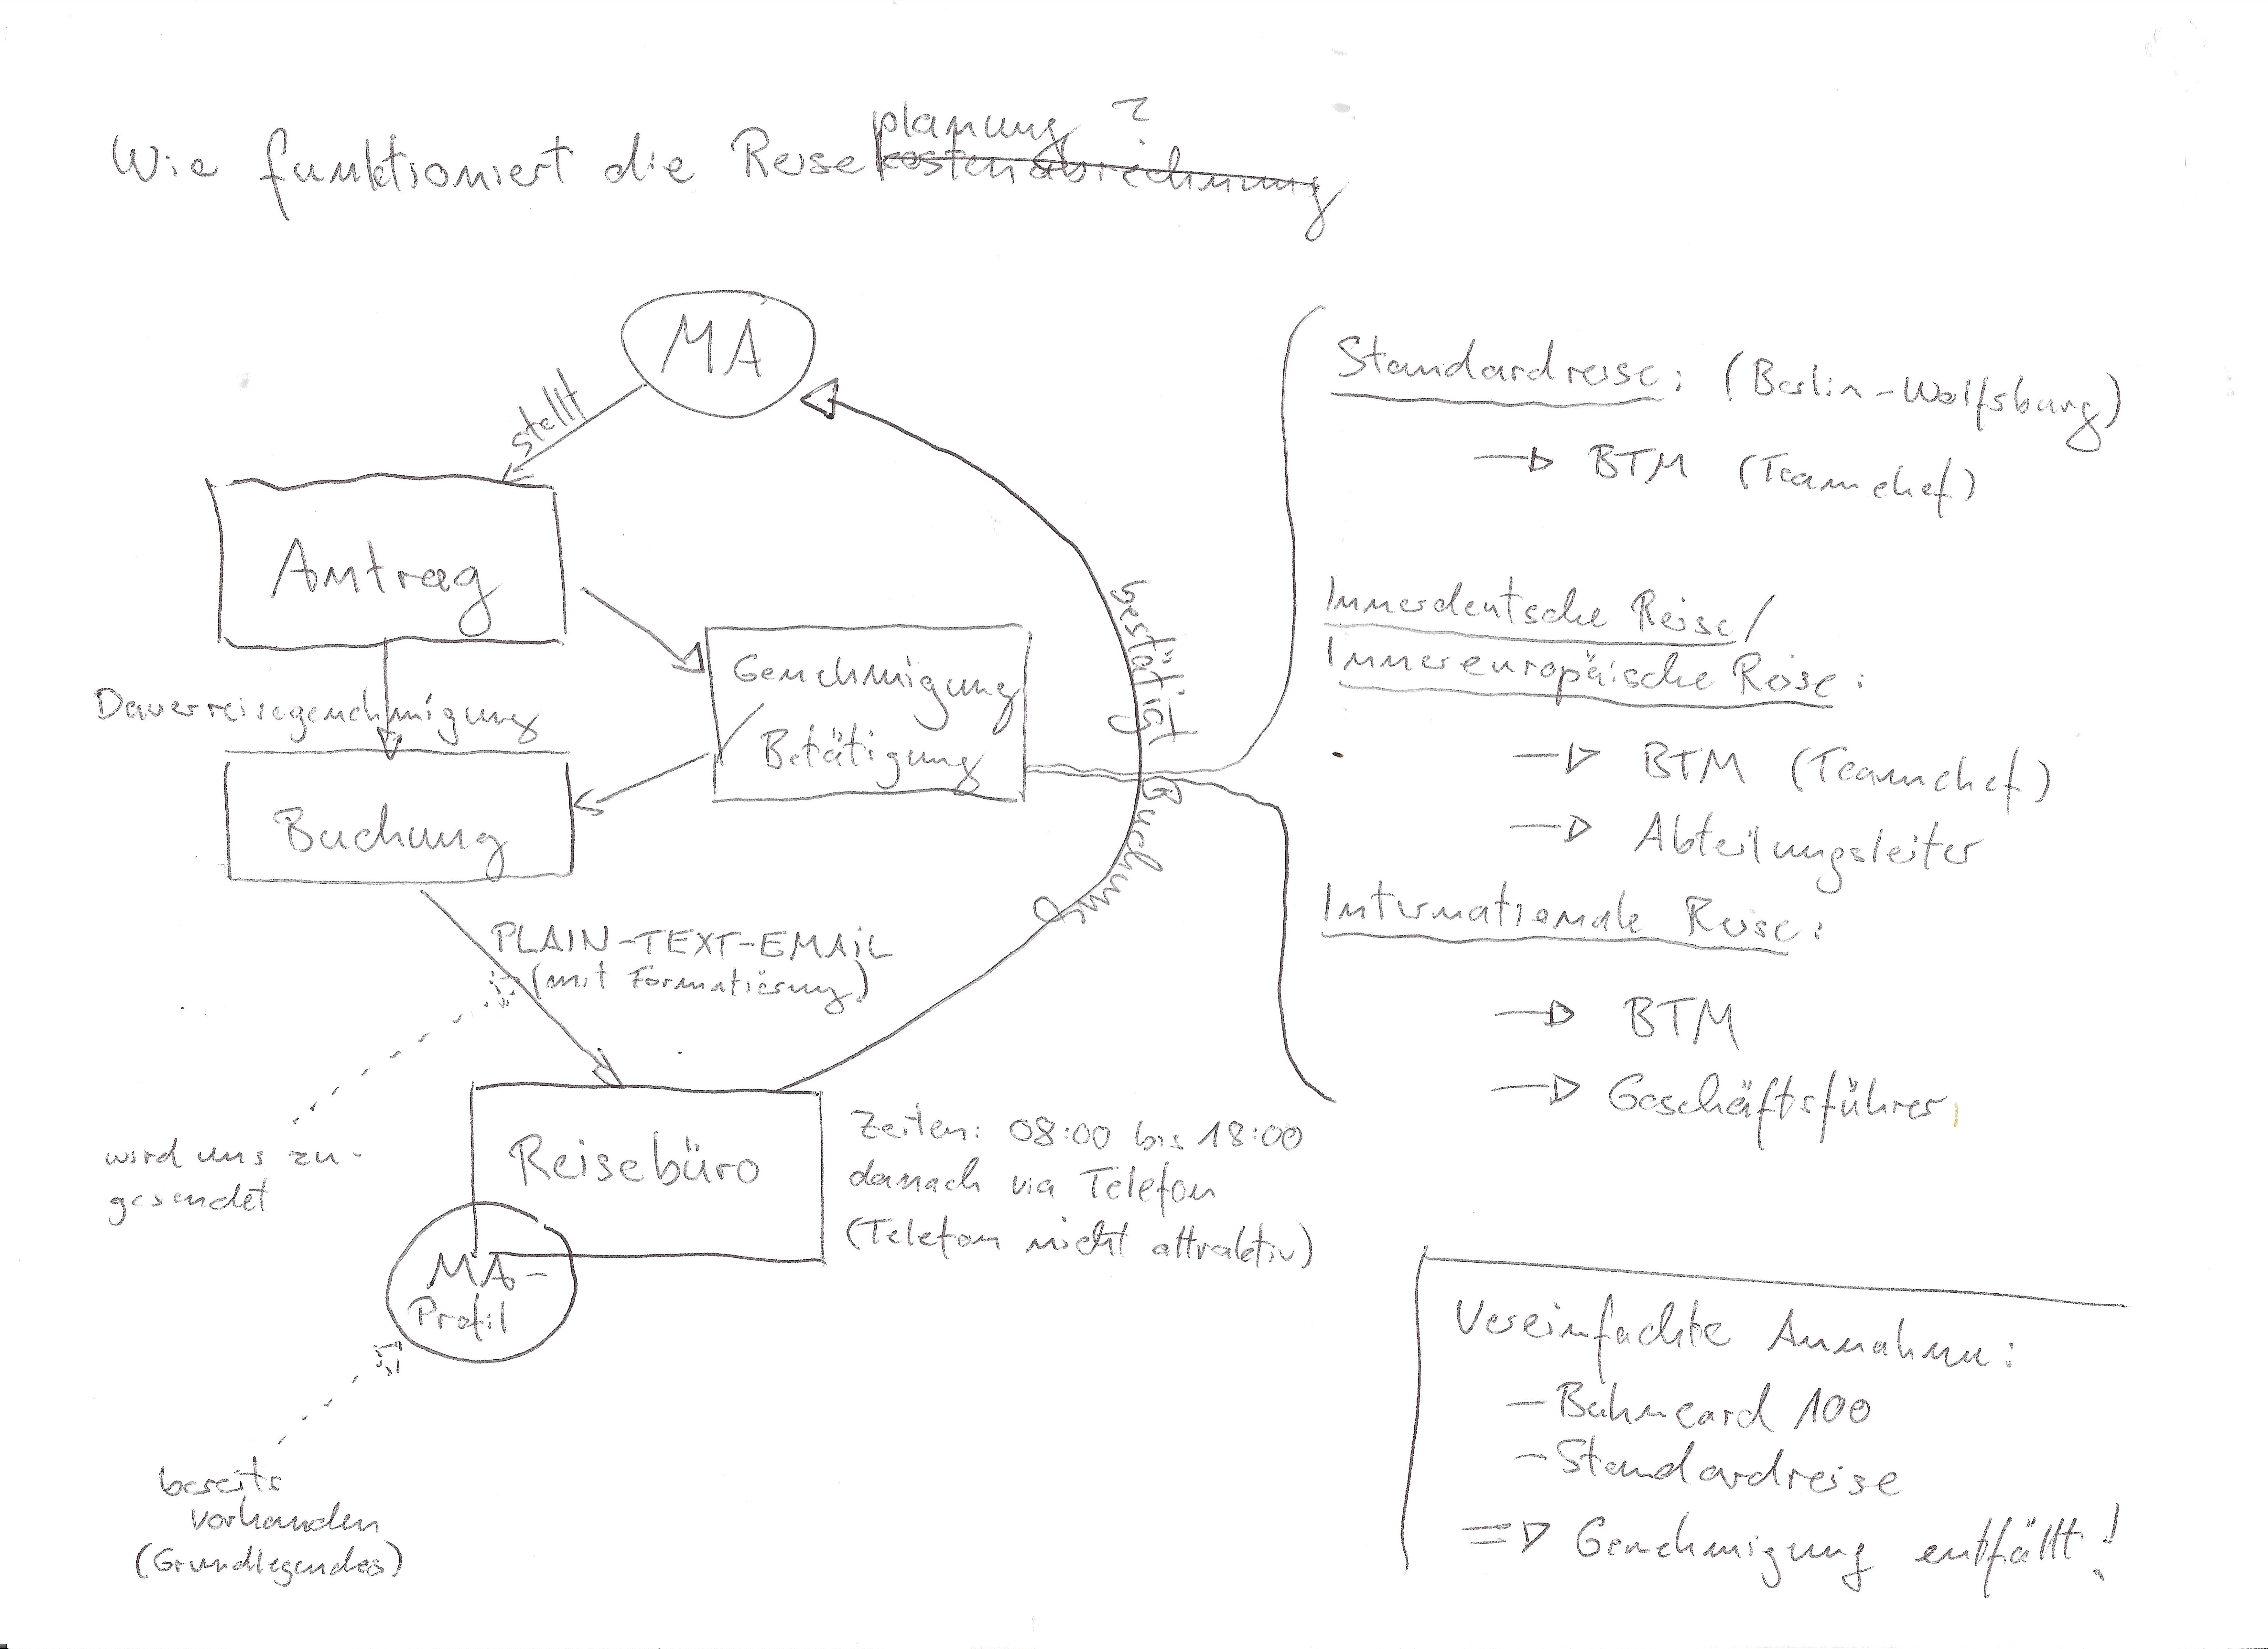
\includegraphics[width=12cm]{04_softwareloesung02_001.jpg}\\
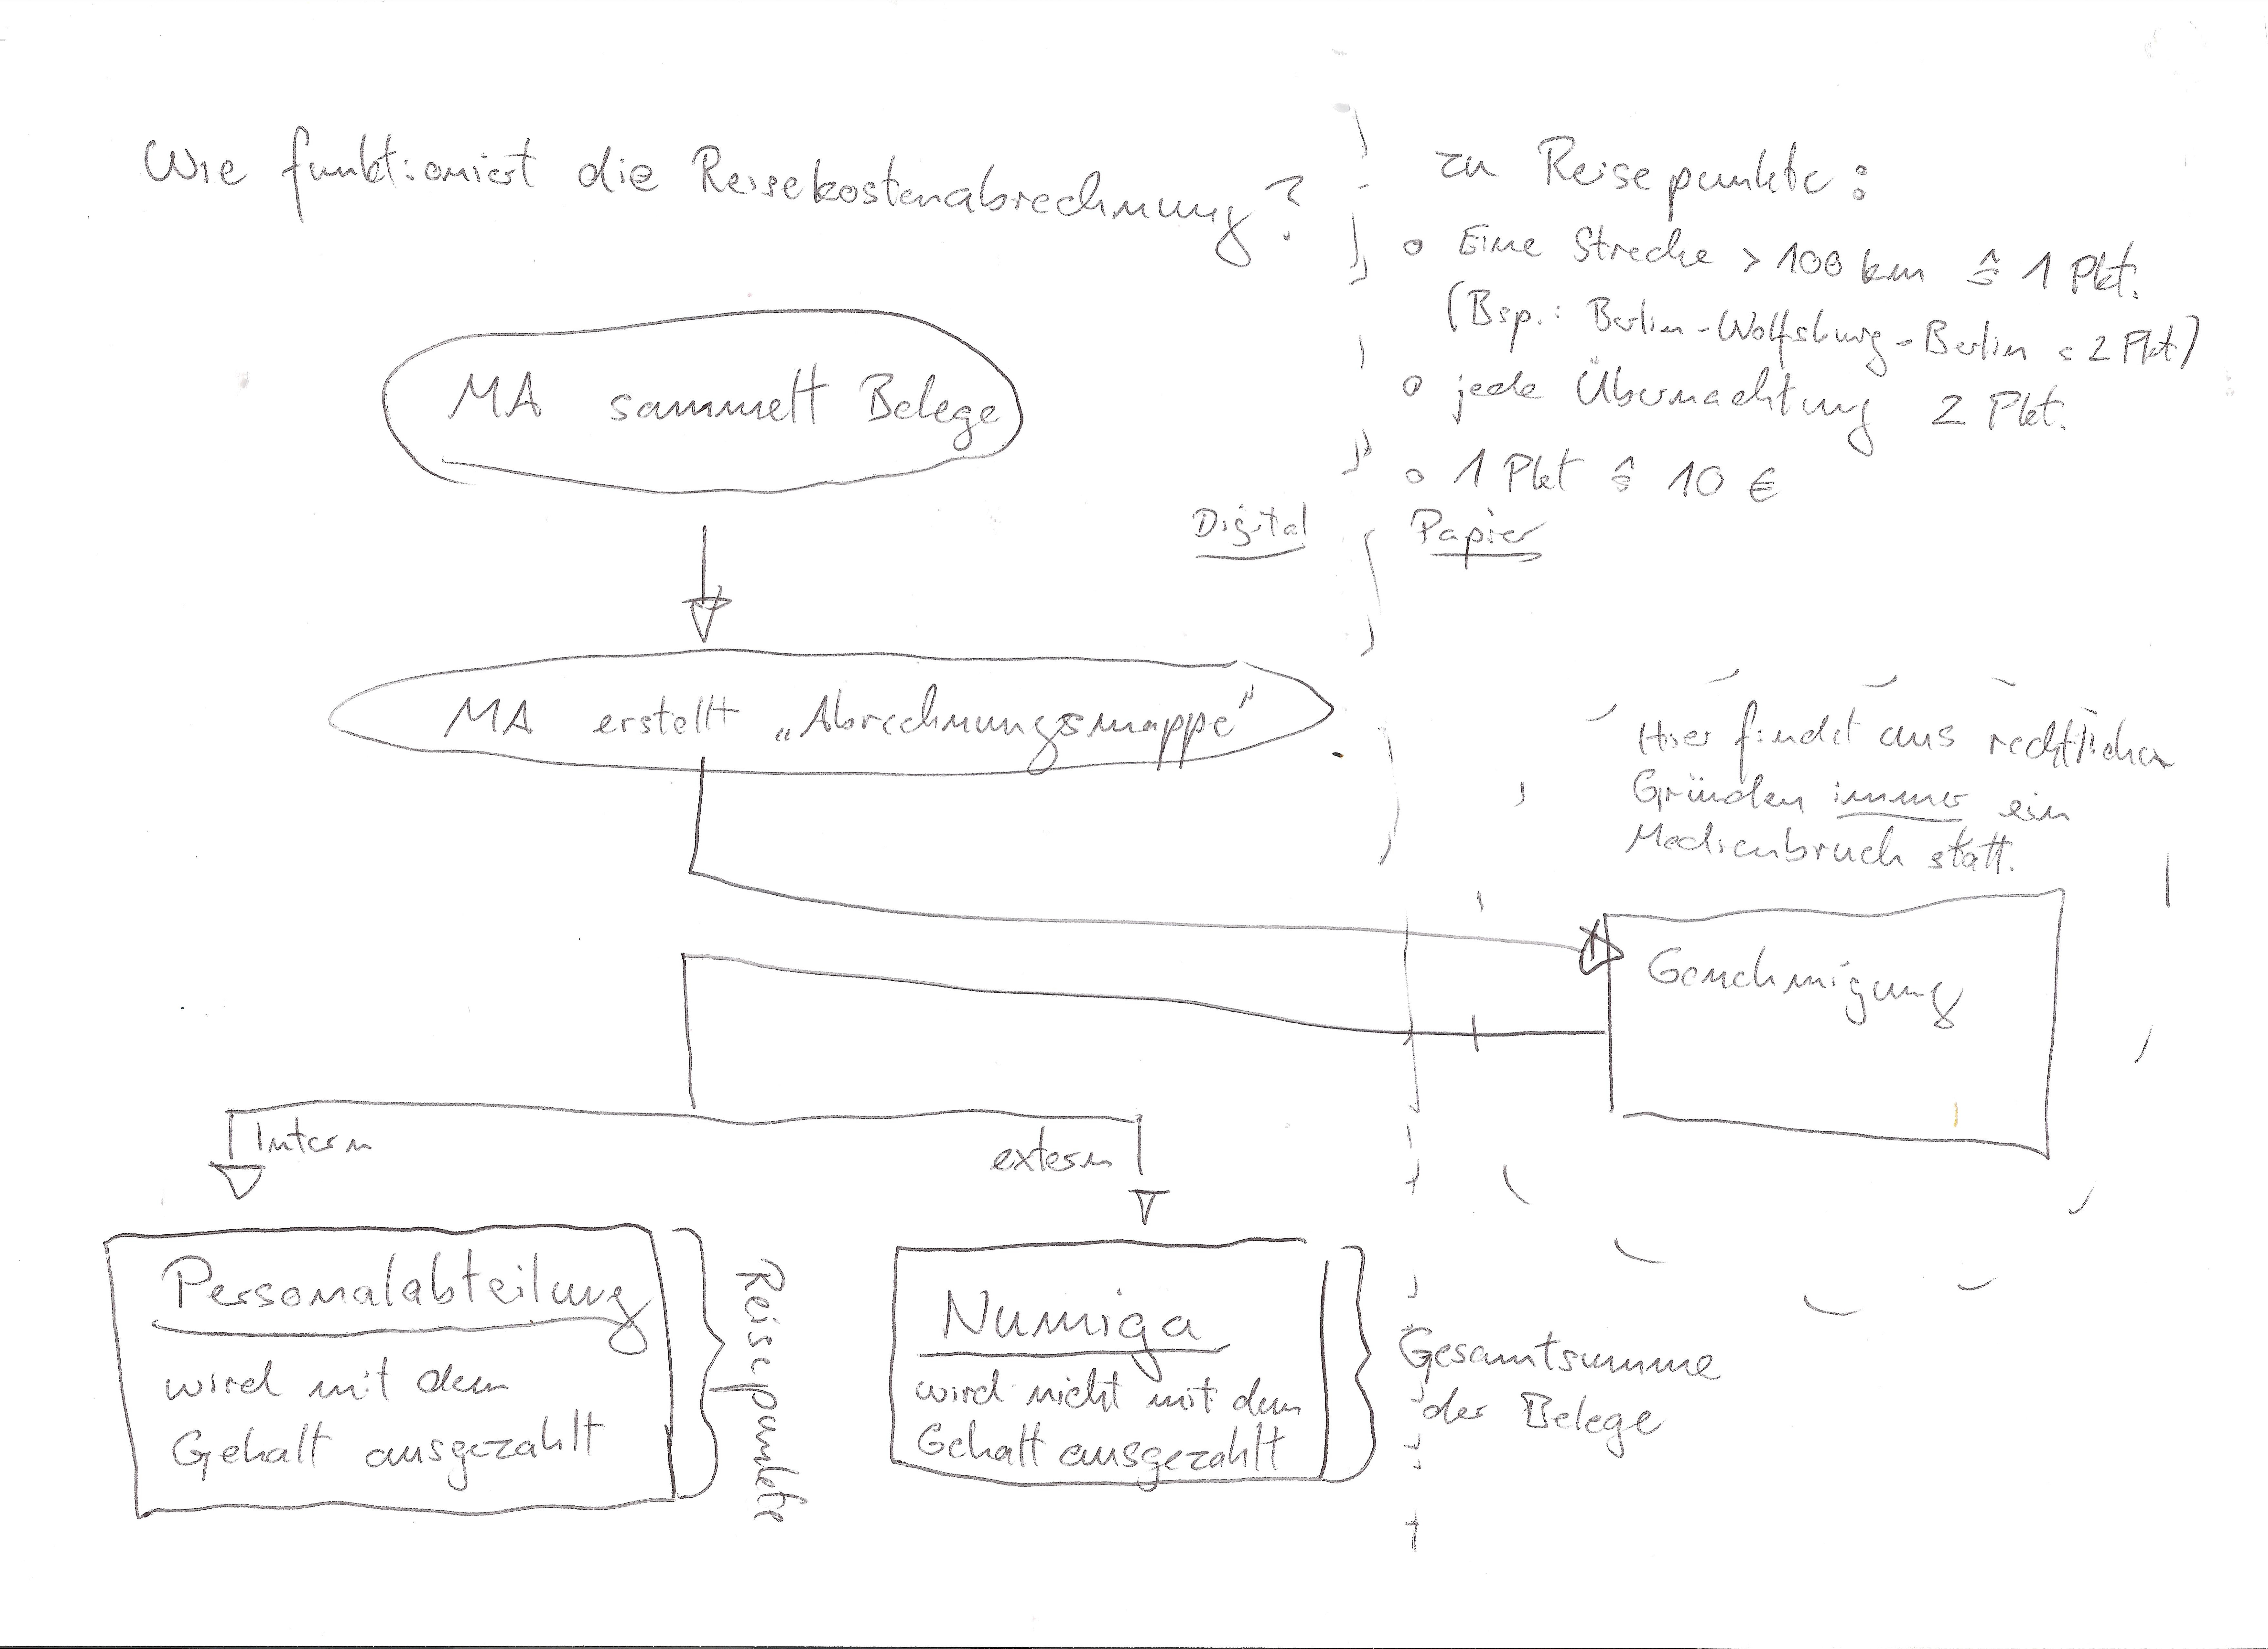
\includegraphics[width=12cm]{04_softwareloesung02_002.jpg}\\
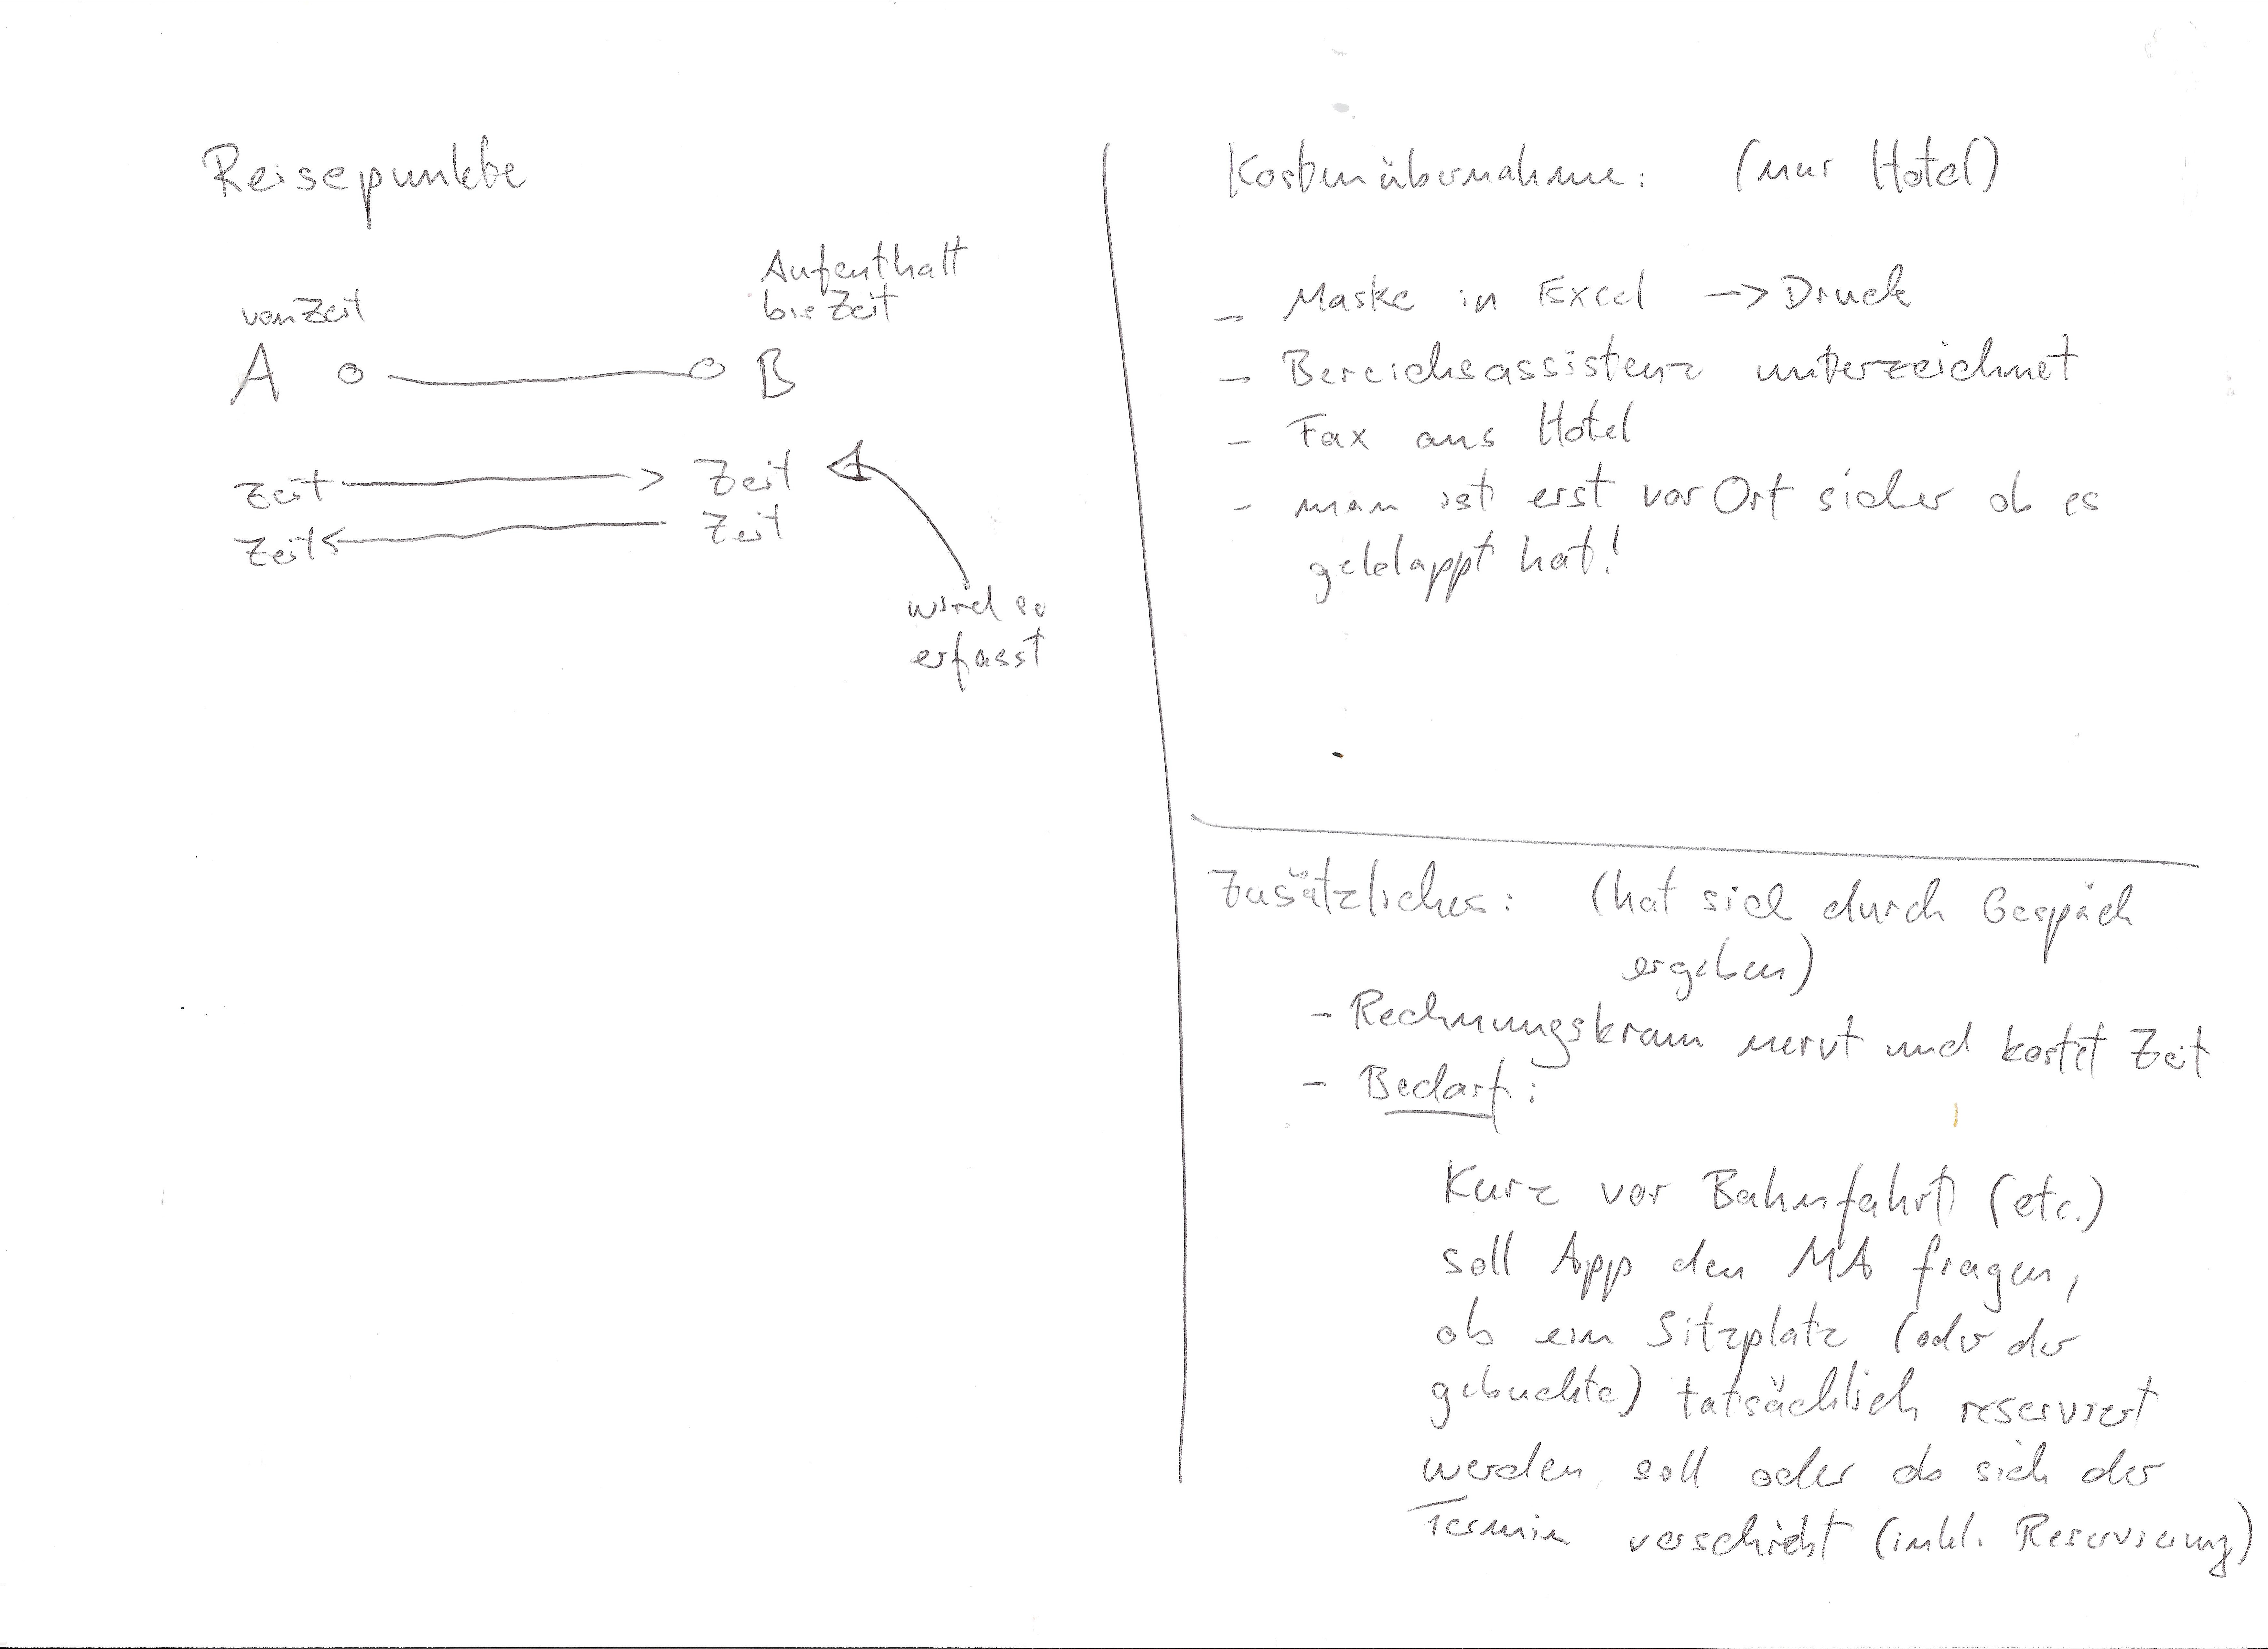
\includegraphics[width=12cm]{04_softwareloesung02_003.jpg}\\
\end{center}
\includepdf[pages=1-18]{05_kick_off_praesentation.pdf}

\section{Phase: Rekonzeption}

In dieser Phase sollten Usability-Tests in Form eines Paper-Prototyping durchgef\"uhrte werden. Da wir durch die misslungene Kick-Off-Pr\"asentation zeitlich zur\"uckgeworfen wurden, mussten wir den Gro\ss teil dieser Phase f\"ur die Rekonzeptionierung verwenden und konnten erst im Anschluss daran mit dem \textit{Paper-Prototyping} beginnen.

\subsection{Woche 04: Kick-Off, Paper-Prototyps}

\subsubsection{Was hat das Team getan?}

Wir haben w\"ahrend der Kick-Off-Veranstaltung unsere Konzepte zwar vorgestellt, konnten aber unsere Ideen nicht vermitteln. Die Pr\"asentation wurde vom Kunden mit der Begr\"undung abgelehnt, dass die Konzepte schlecht ausgearbeitet sein.\\
Zwei Teammitglieder haben unabh\"angig von einander \textit{Paper-Prototyps} entworfen, die anschlie\ss end zusammengef\"uhrt wurden. Wir haben die einzelnen \textit{Paper-Prototyps} mit Mitarbeitern der Carmeq GmbH getestet und anschlie\ss end alle \textit{Paper-Prototypen} zu einem \textit{konvergenten Paper-Prototypen} zusammengef\"uhrt.

\subsubsection{Zentrale Entscheidungen}

Wir haben zu erst verschiedene \textit{Paper-Prototypen} entwickelt und diese anschlie\ss end zu einem \textit{konvergenten Paper-Prototypen} zusammengef\"uhrt um aus einer gr\"o\ss eren Menge von Ideen sch\"opfen zu k\"onnen. 

\subsection{Ergebnisse dieser Phase}

Wir haben mehrere \textit{Papier-Prototypen} entwickelt, beim Kunden getestet und daraus \textit{Userstories} mit einer groben Aufwandabsch\"atzung abgeleitet.

\begin{itemize}
\item Paper-Prototyps (PDF)
\item Verhaltensanalysen (PDF)
\item konvergenter Paper-Prototyp (PNG)
\item Userstories und Szenarien (PDF)
\end{itemize}

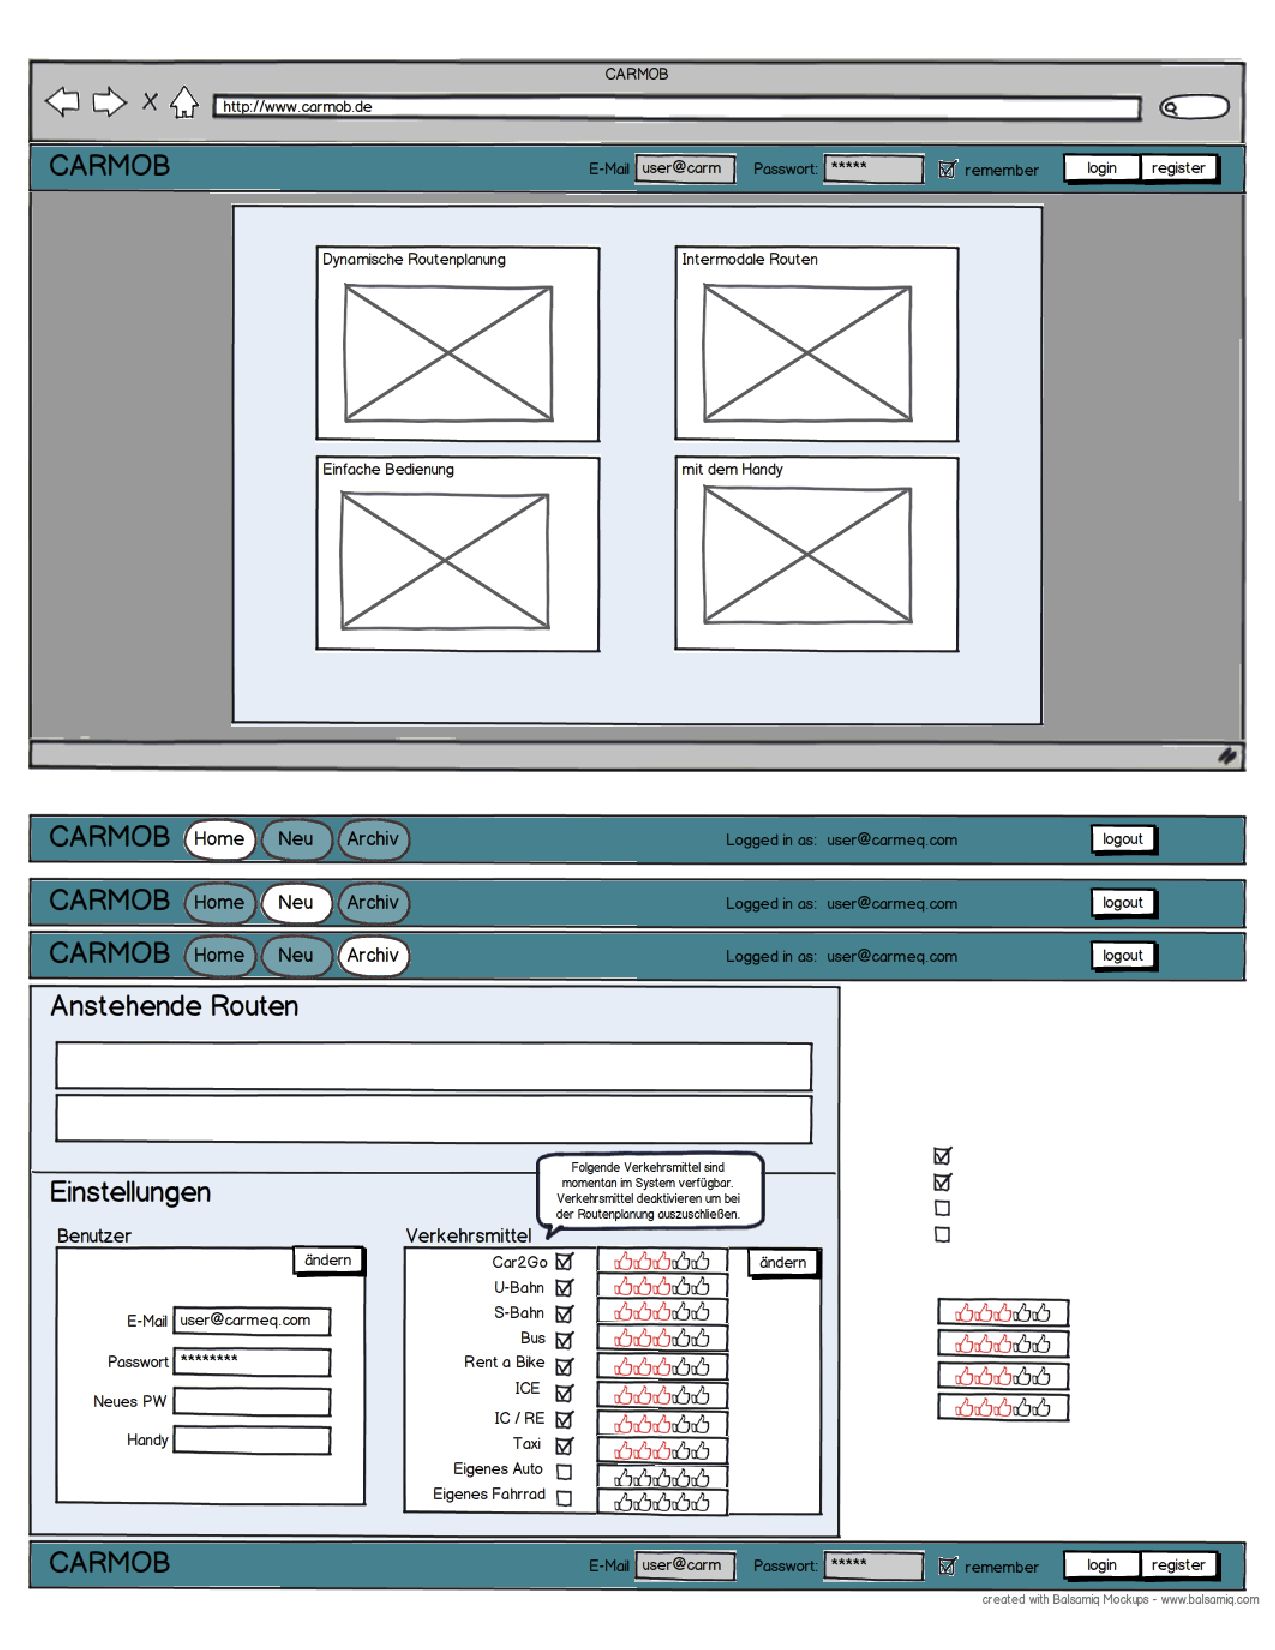
\includepdf[pages=1-1]{06_paperprototyp01_000.pdf}
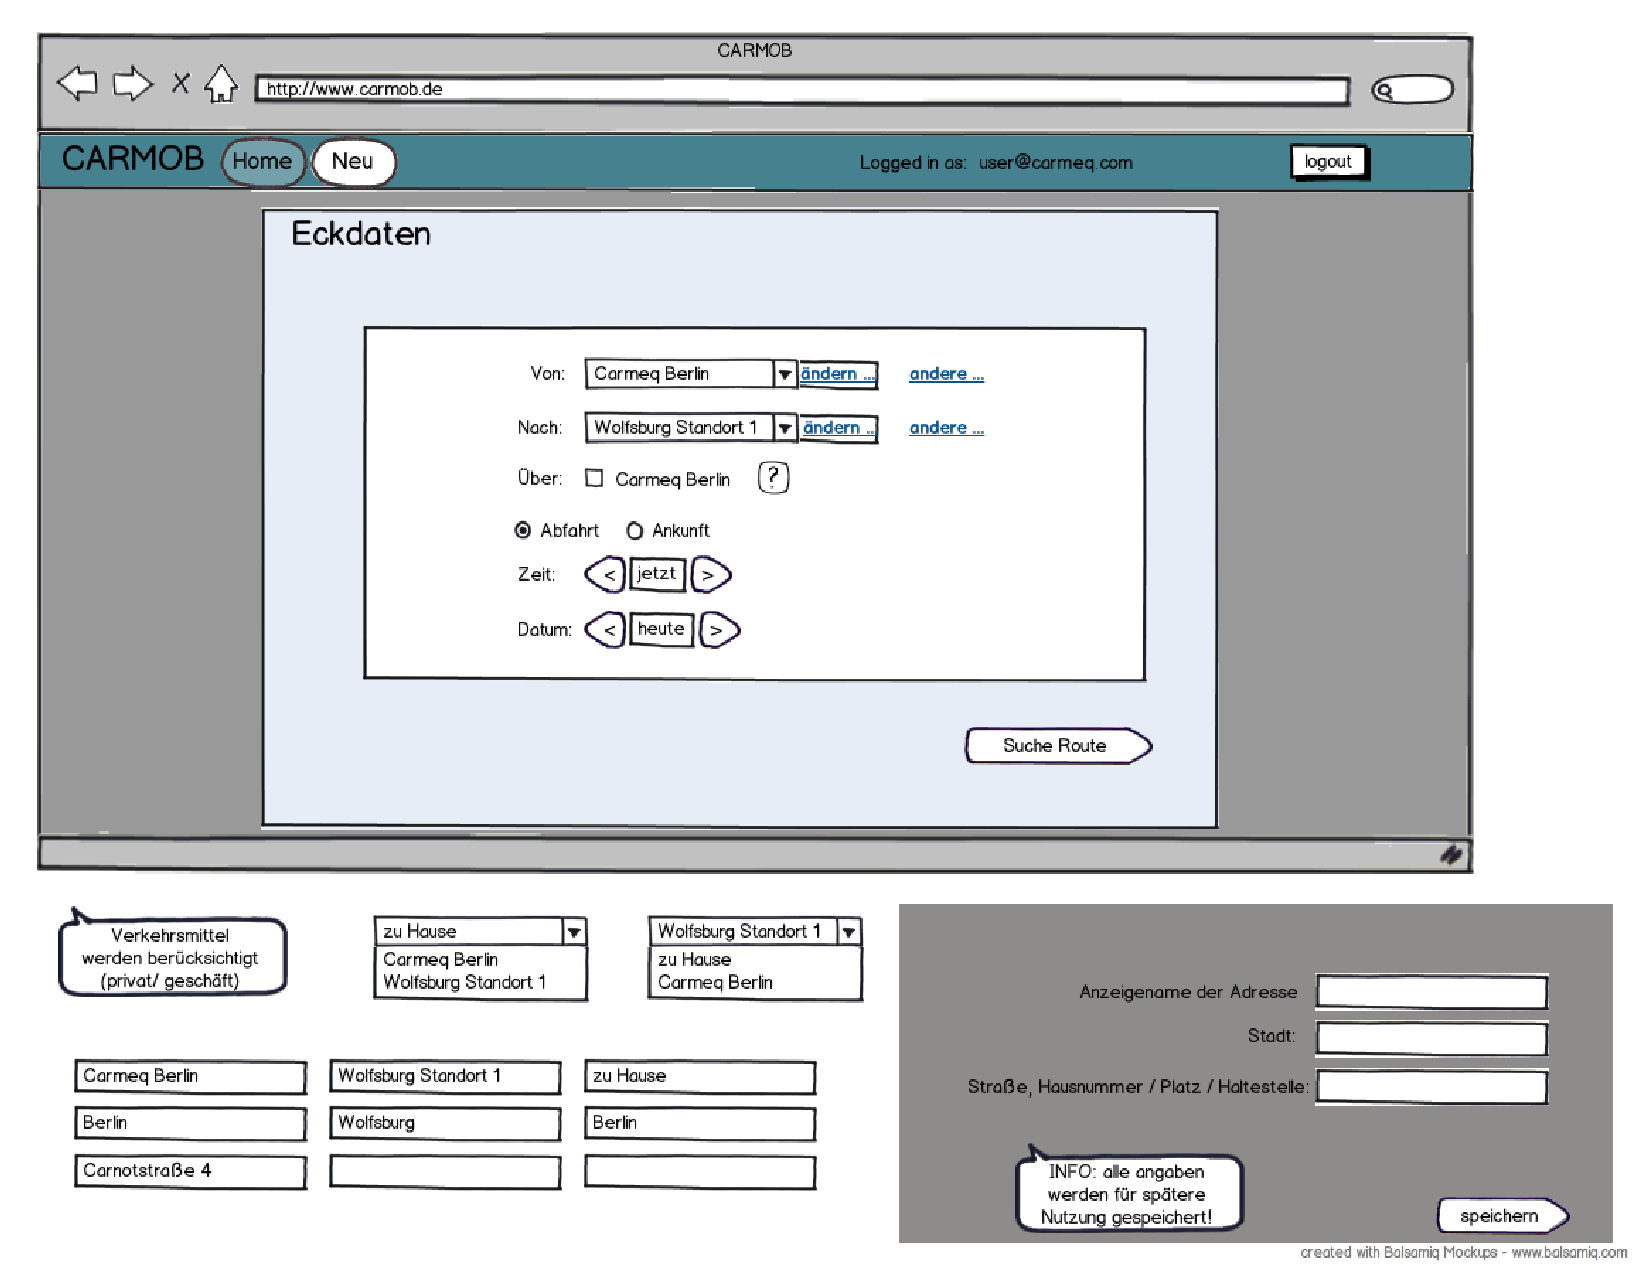
\includepdf[pages=1-1]{06_paperprototyp01_001.pdf}
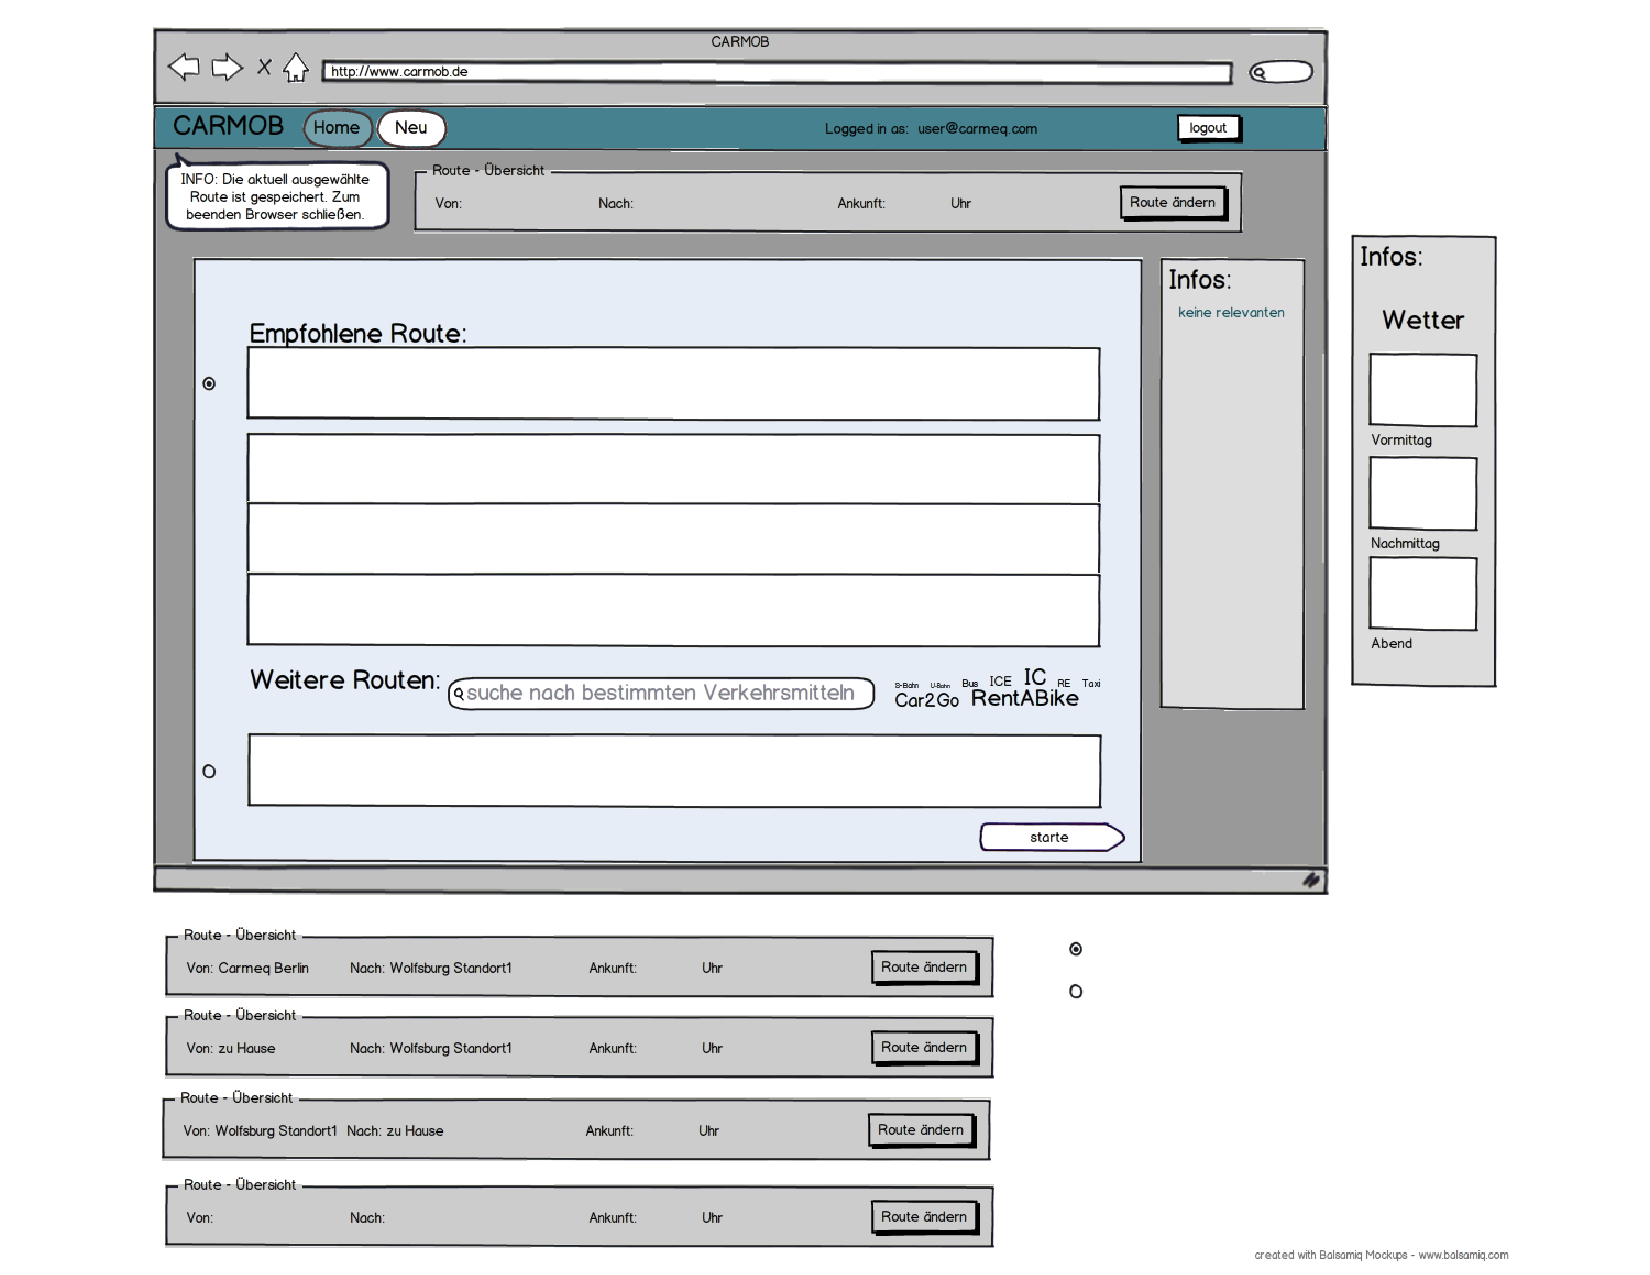
\includepdf[pages=1-1]{06_paperprototyp01_002.pdf}
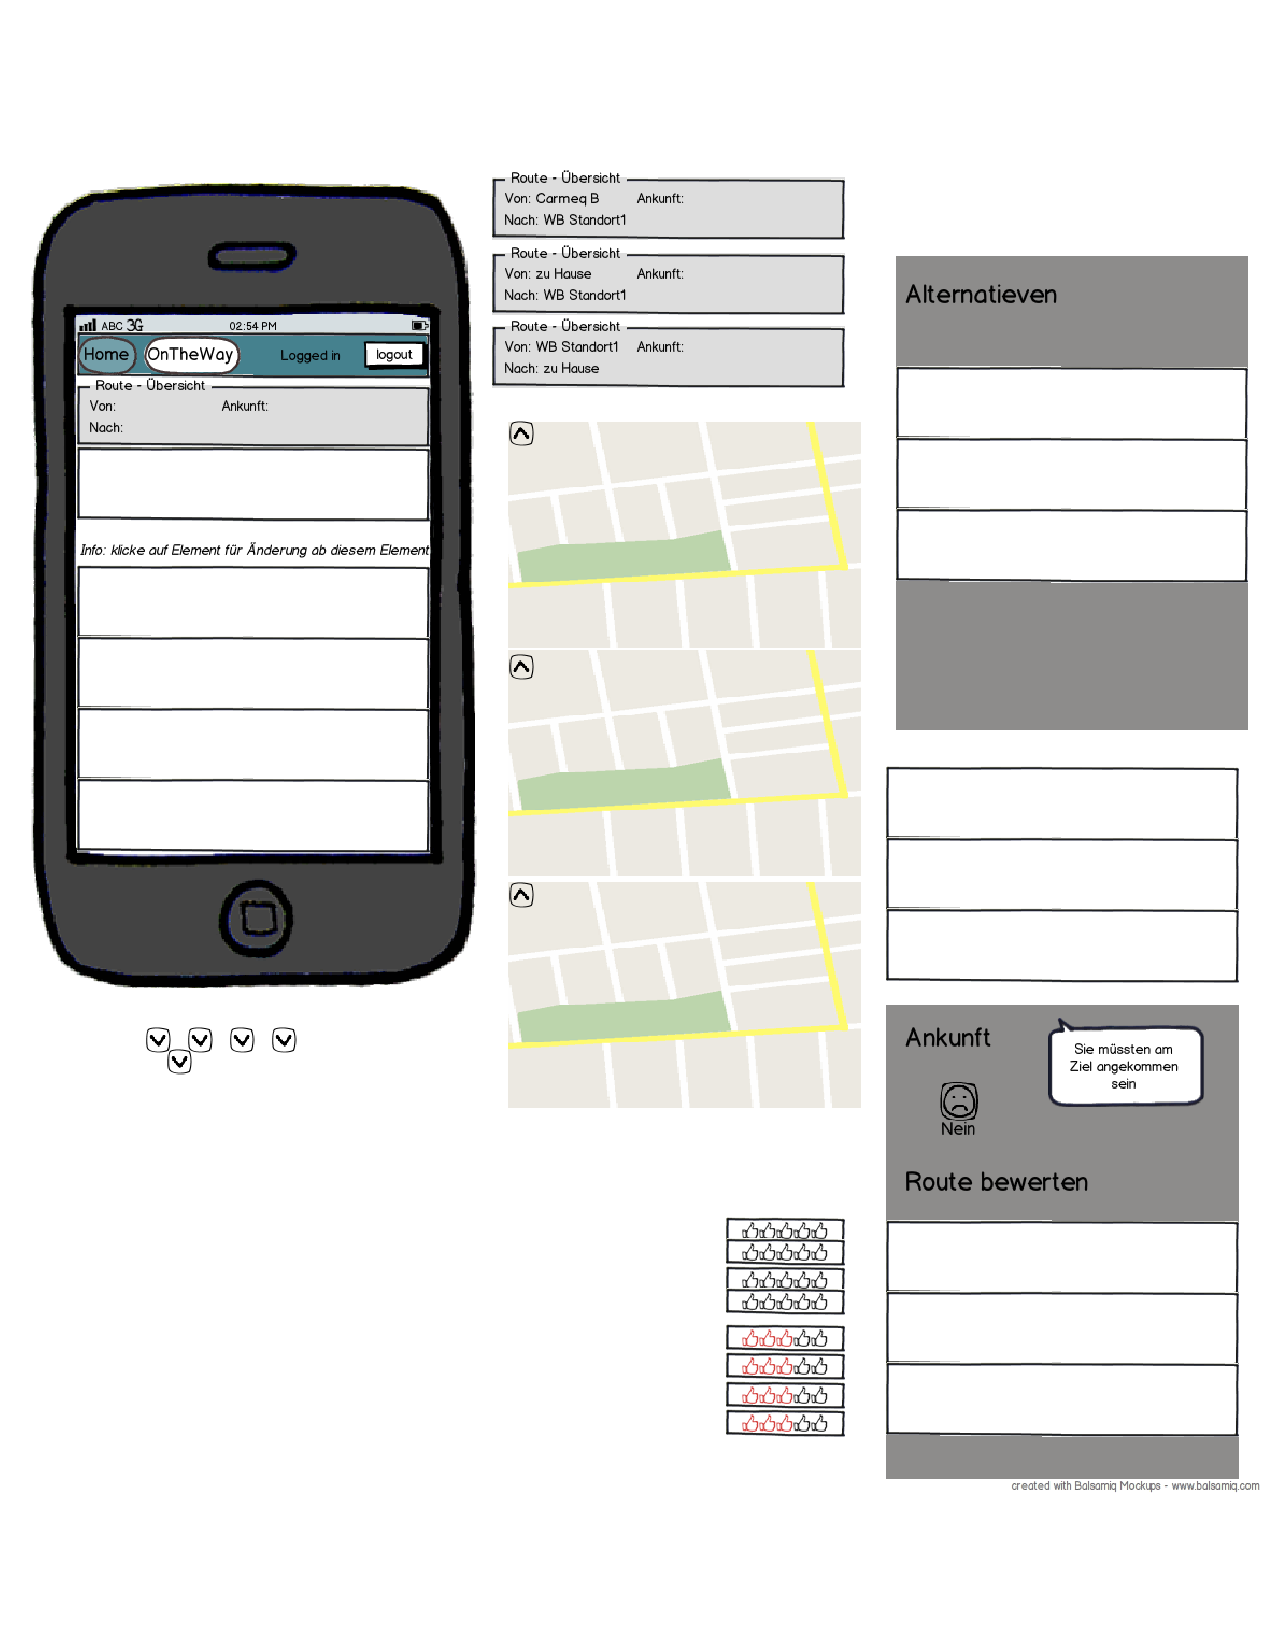
\includepdf[pages=1-1]{06_paperprototyp01_003.pdf}
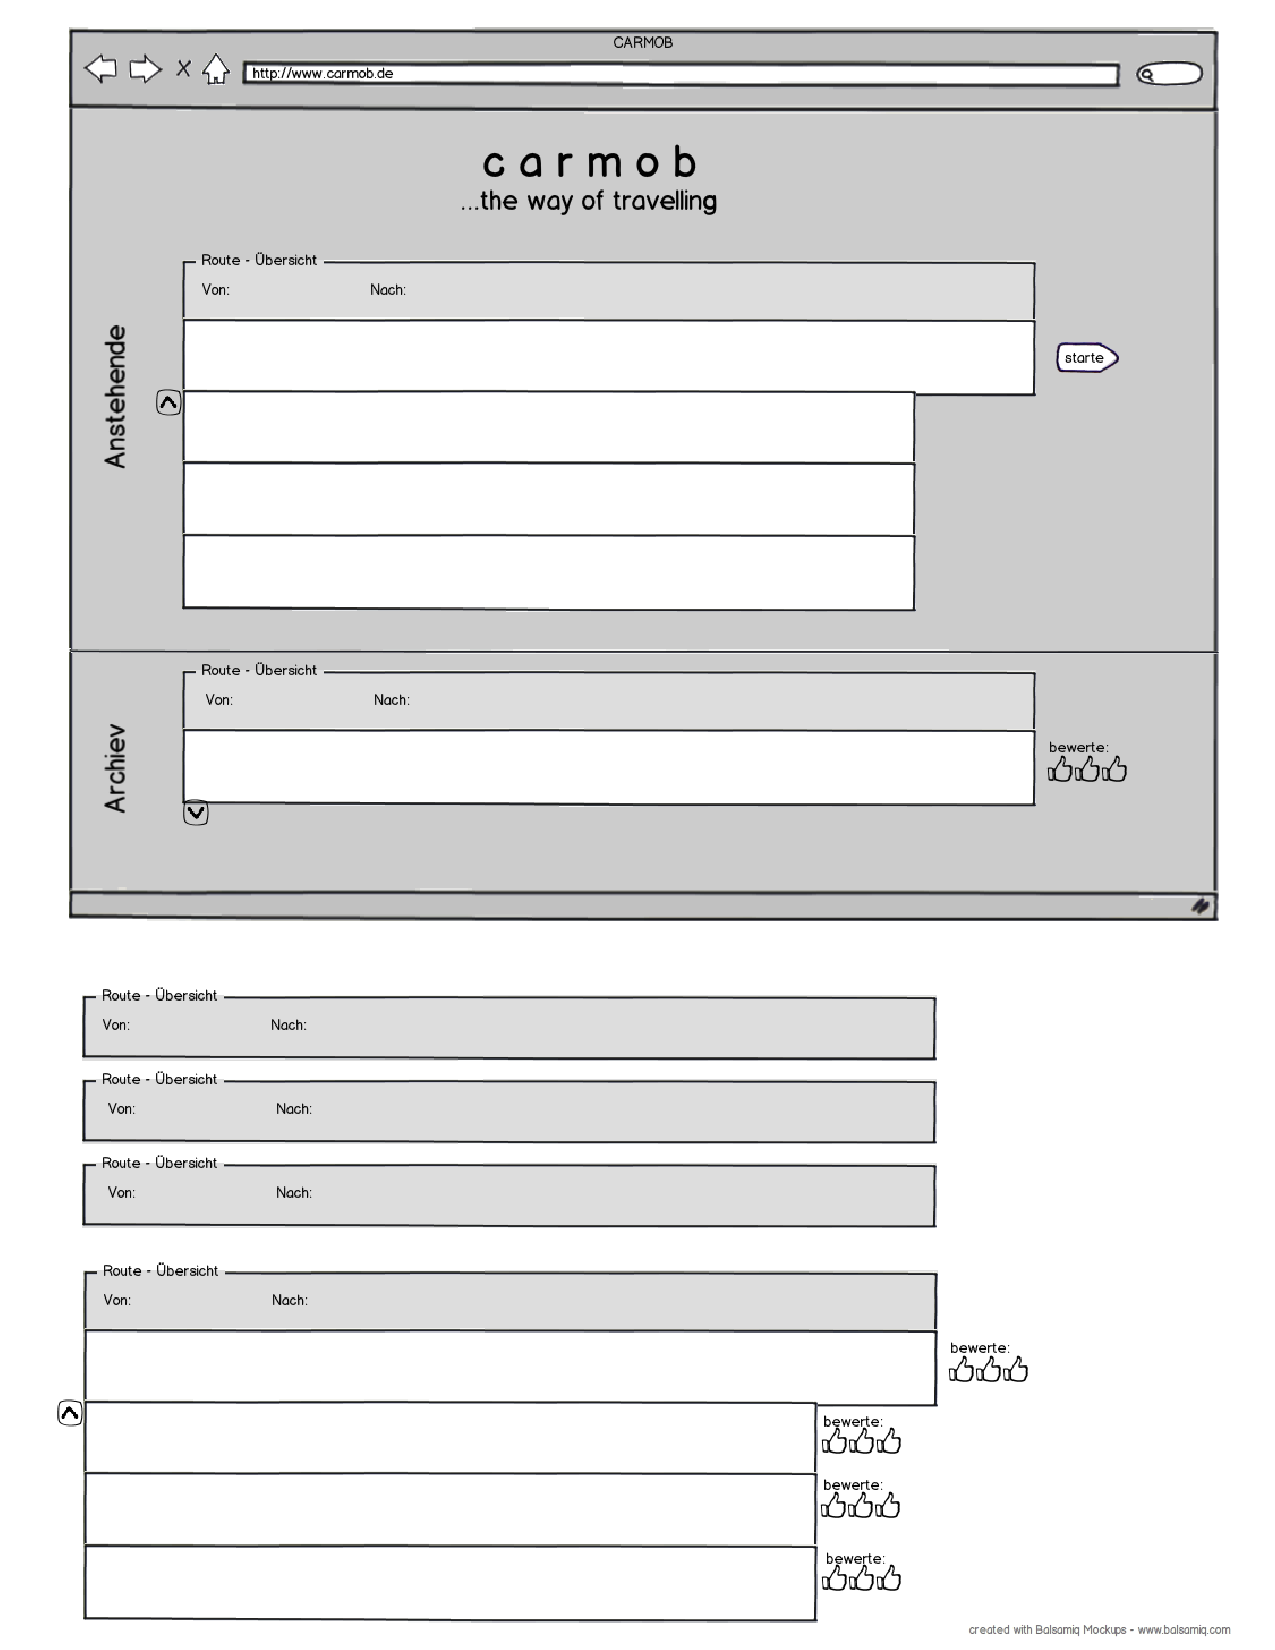
\includepdf[pages=1-1]{06_paperprototyp01_004.pdf}
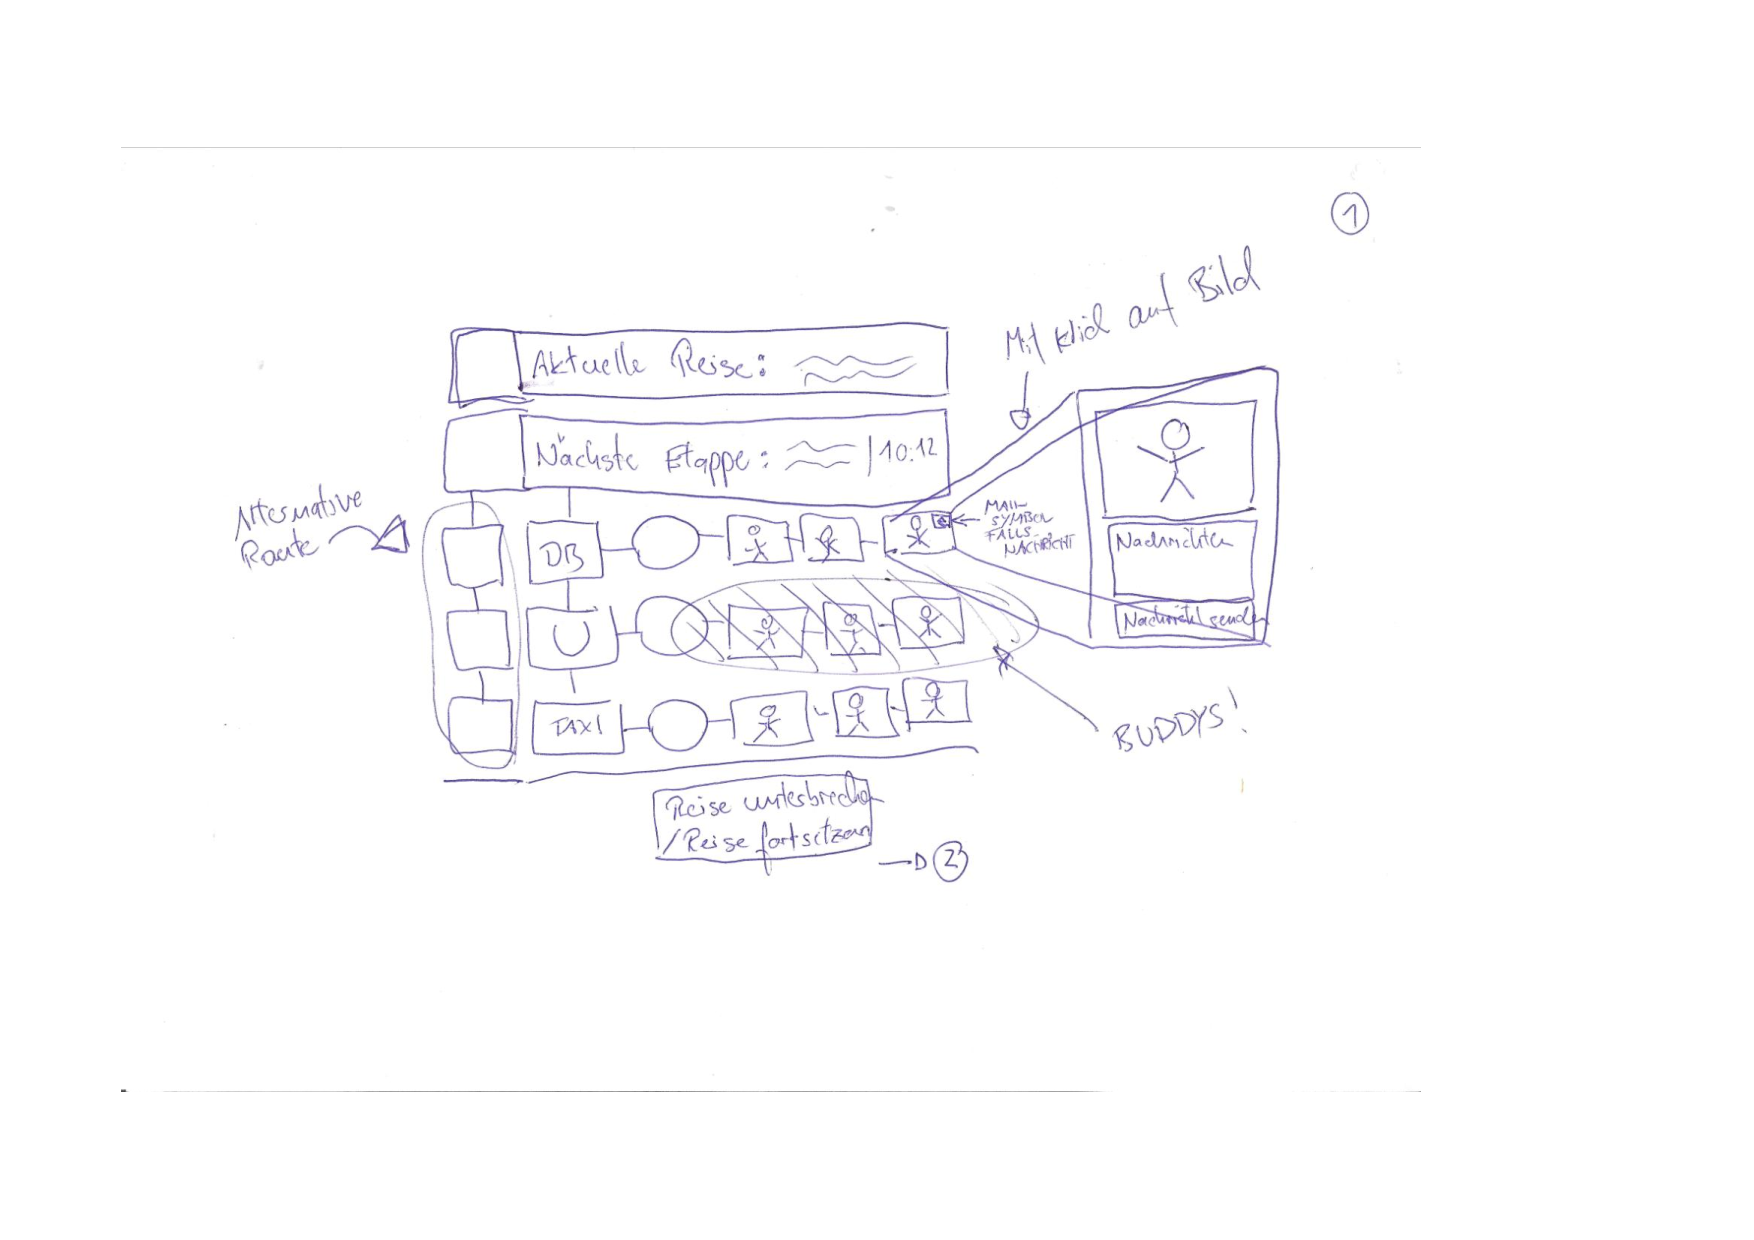
\includepdf[pages=1-5]{06_paperprototyp02.pdf}
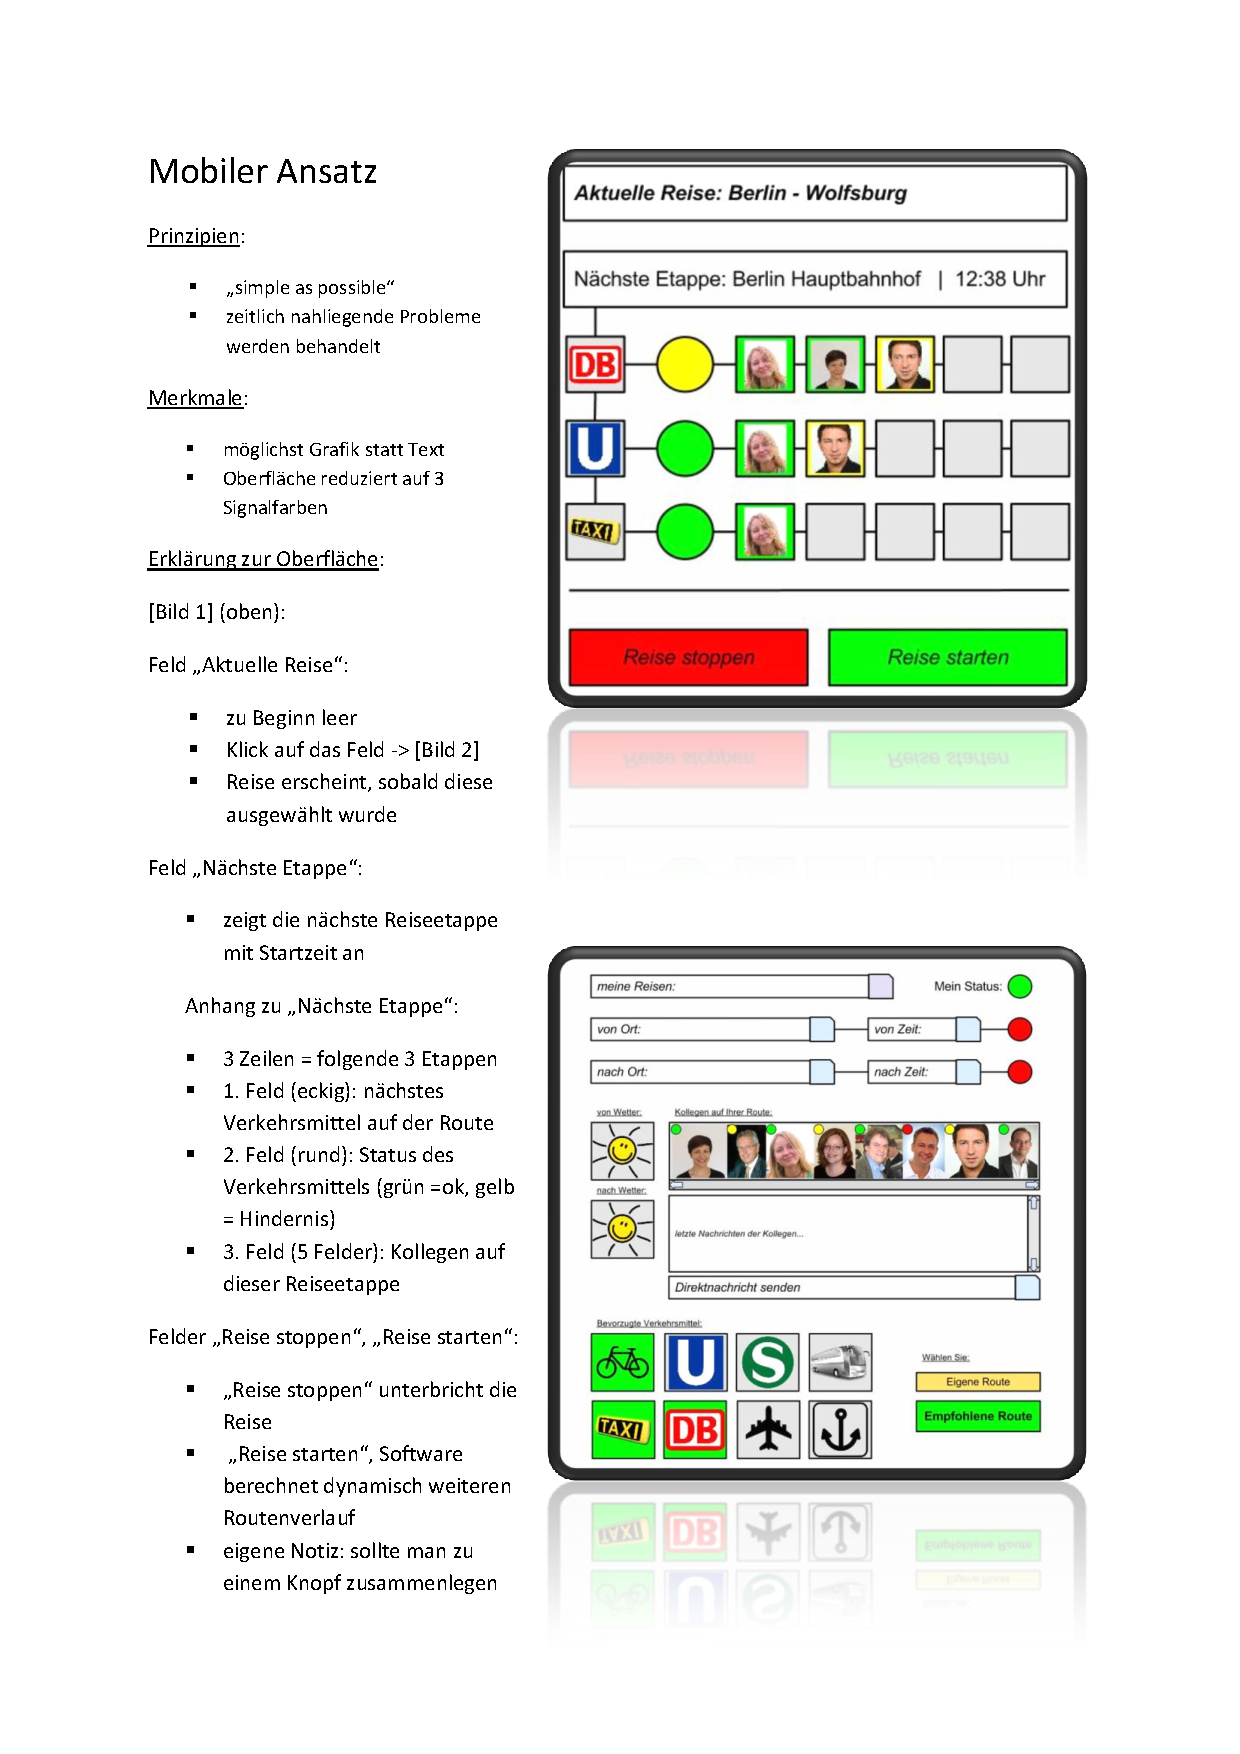
\includepdf[pages=1-3]{06_paperprototyp03.pdf}
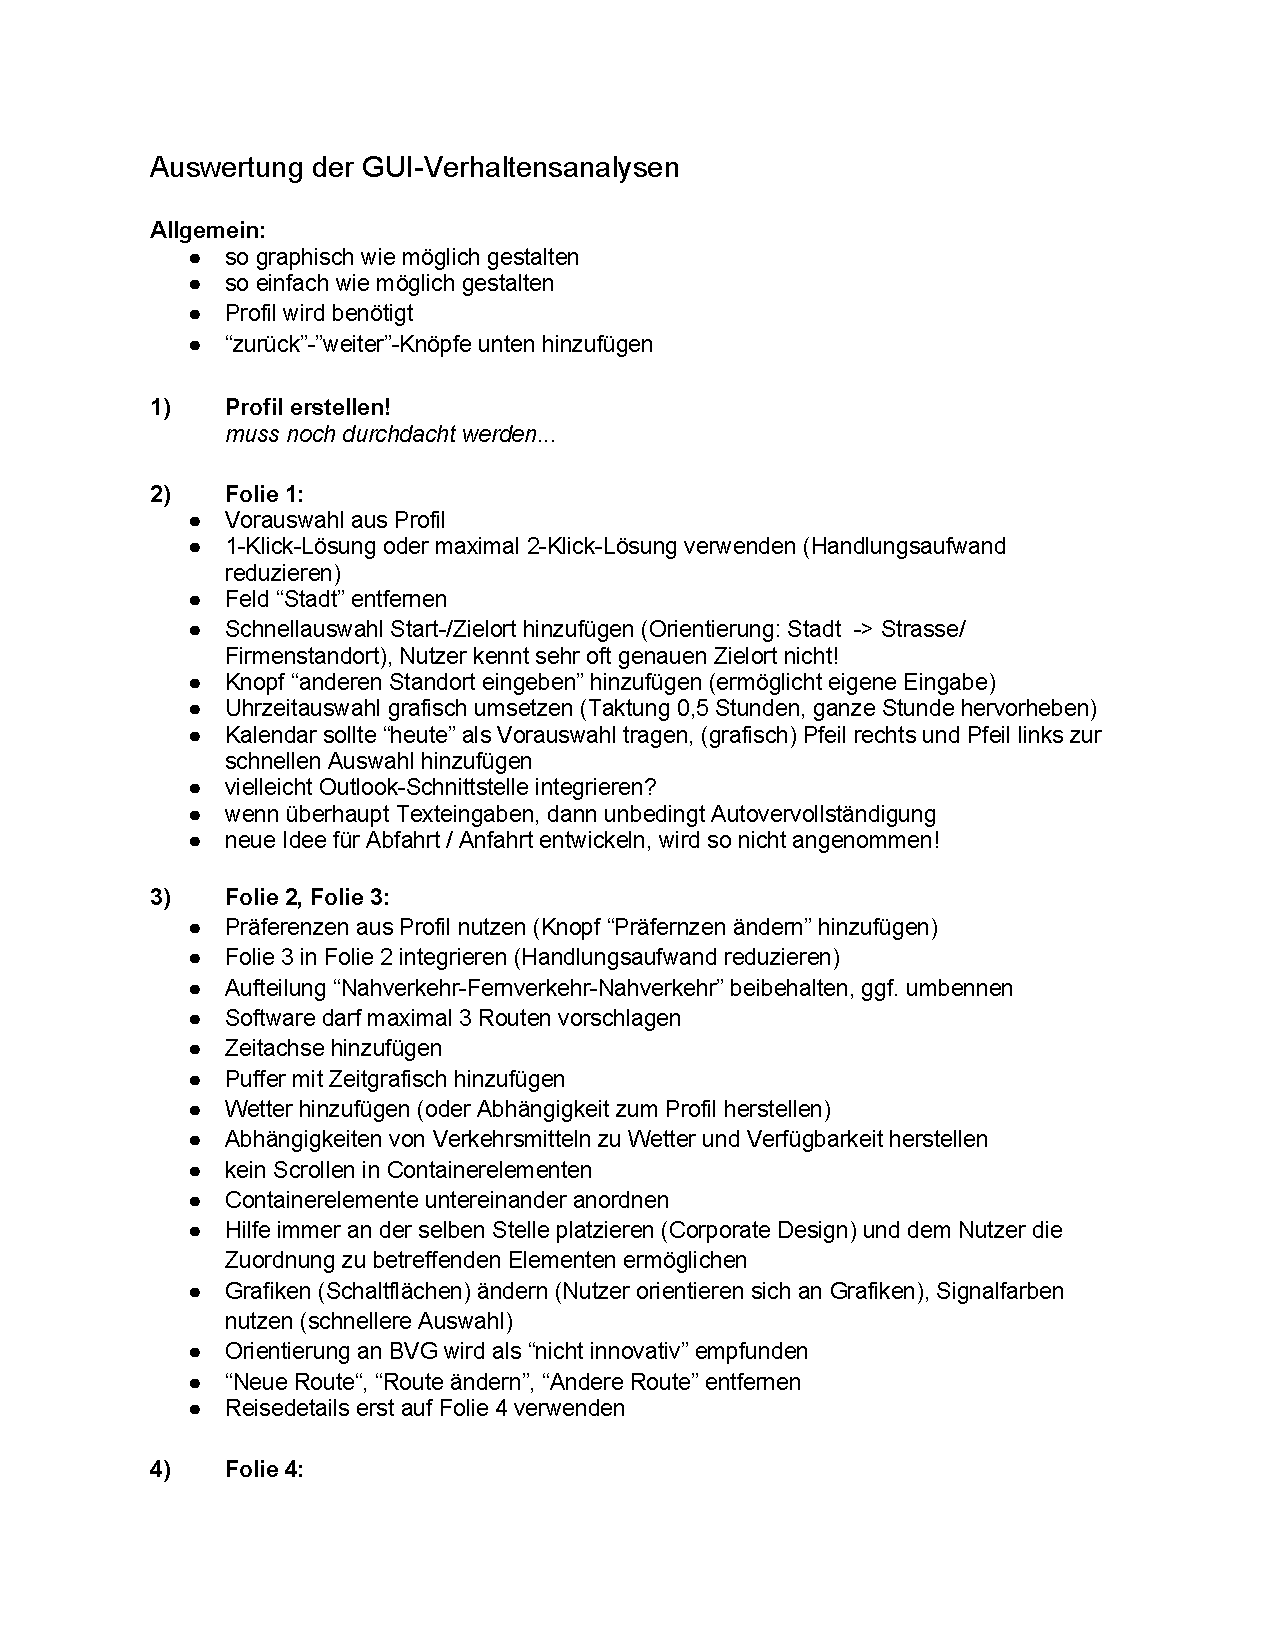
\includepdf[pages=1-2]{07_verhaltensanalyse01.pdf}
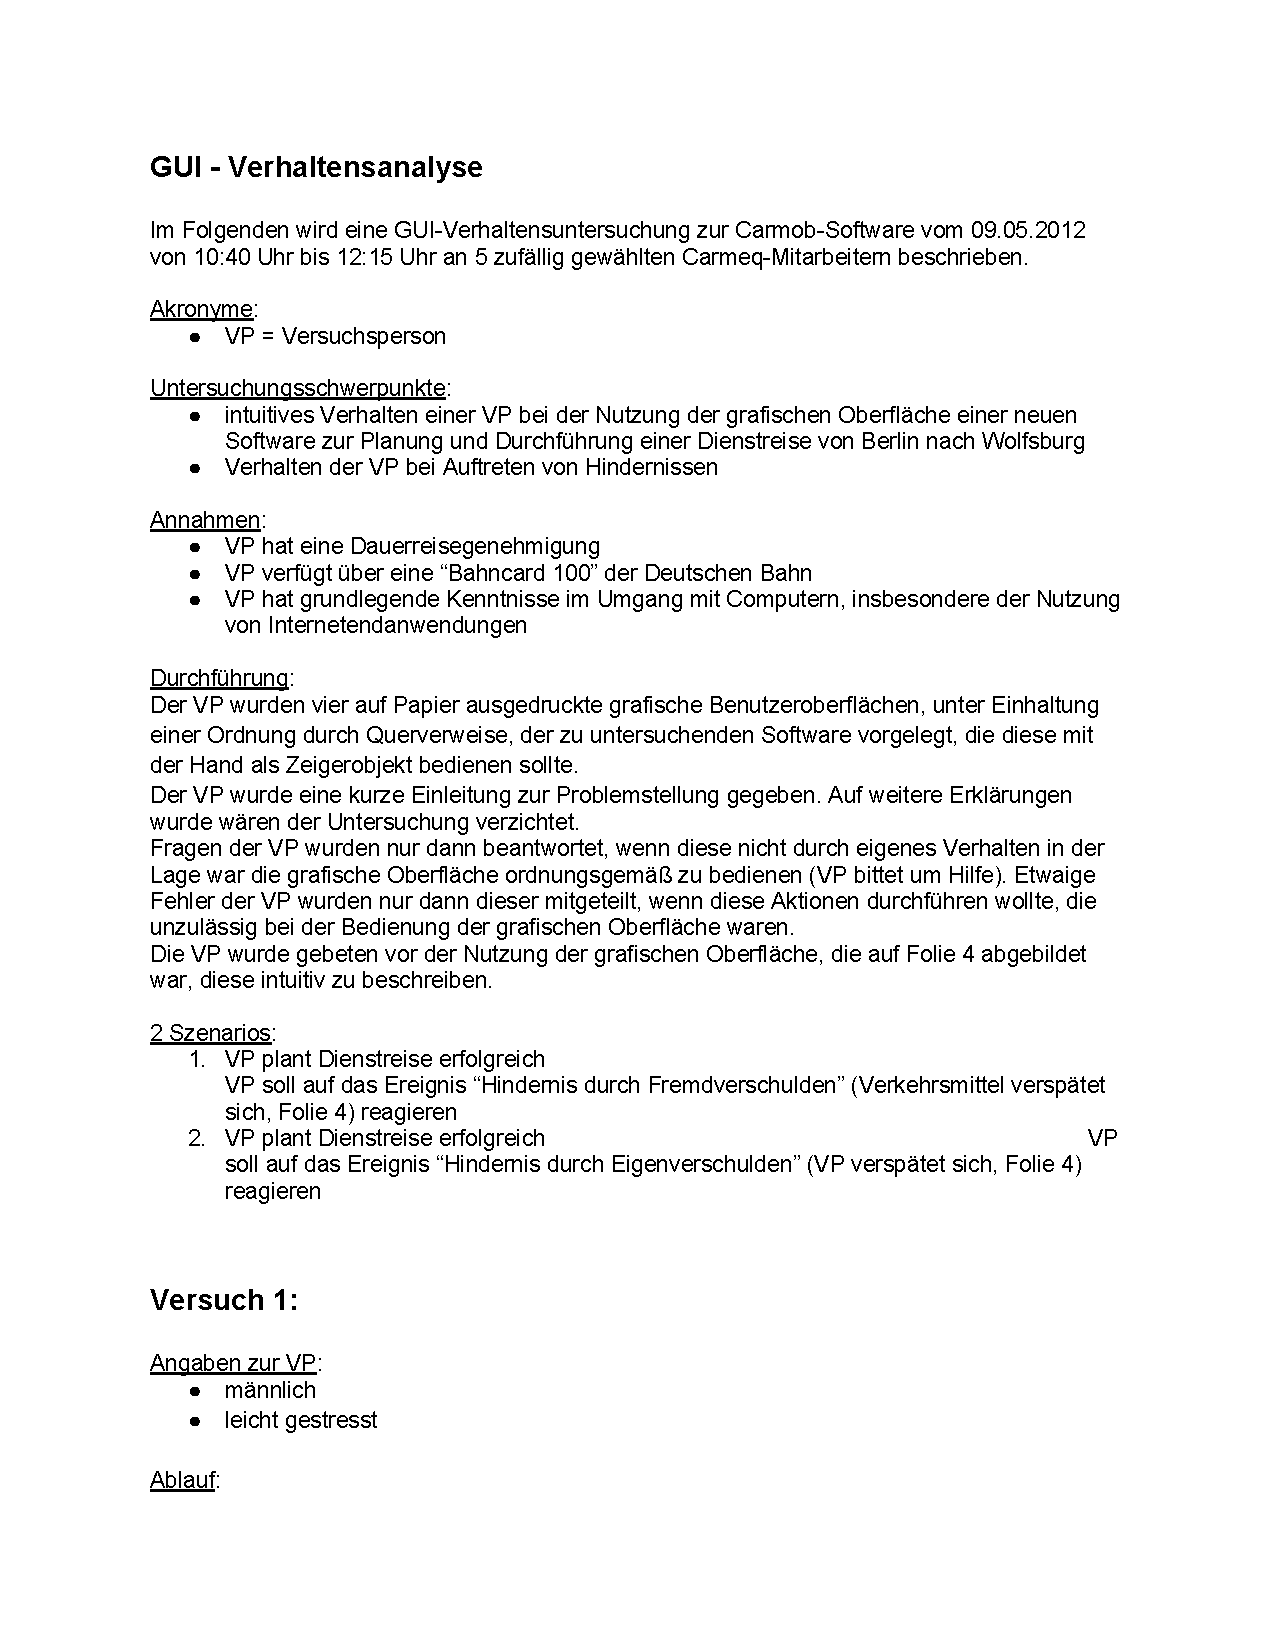
\includepdf[pages=1-7]{07_verhaltensanalyse02.pdf}
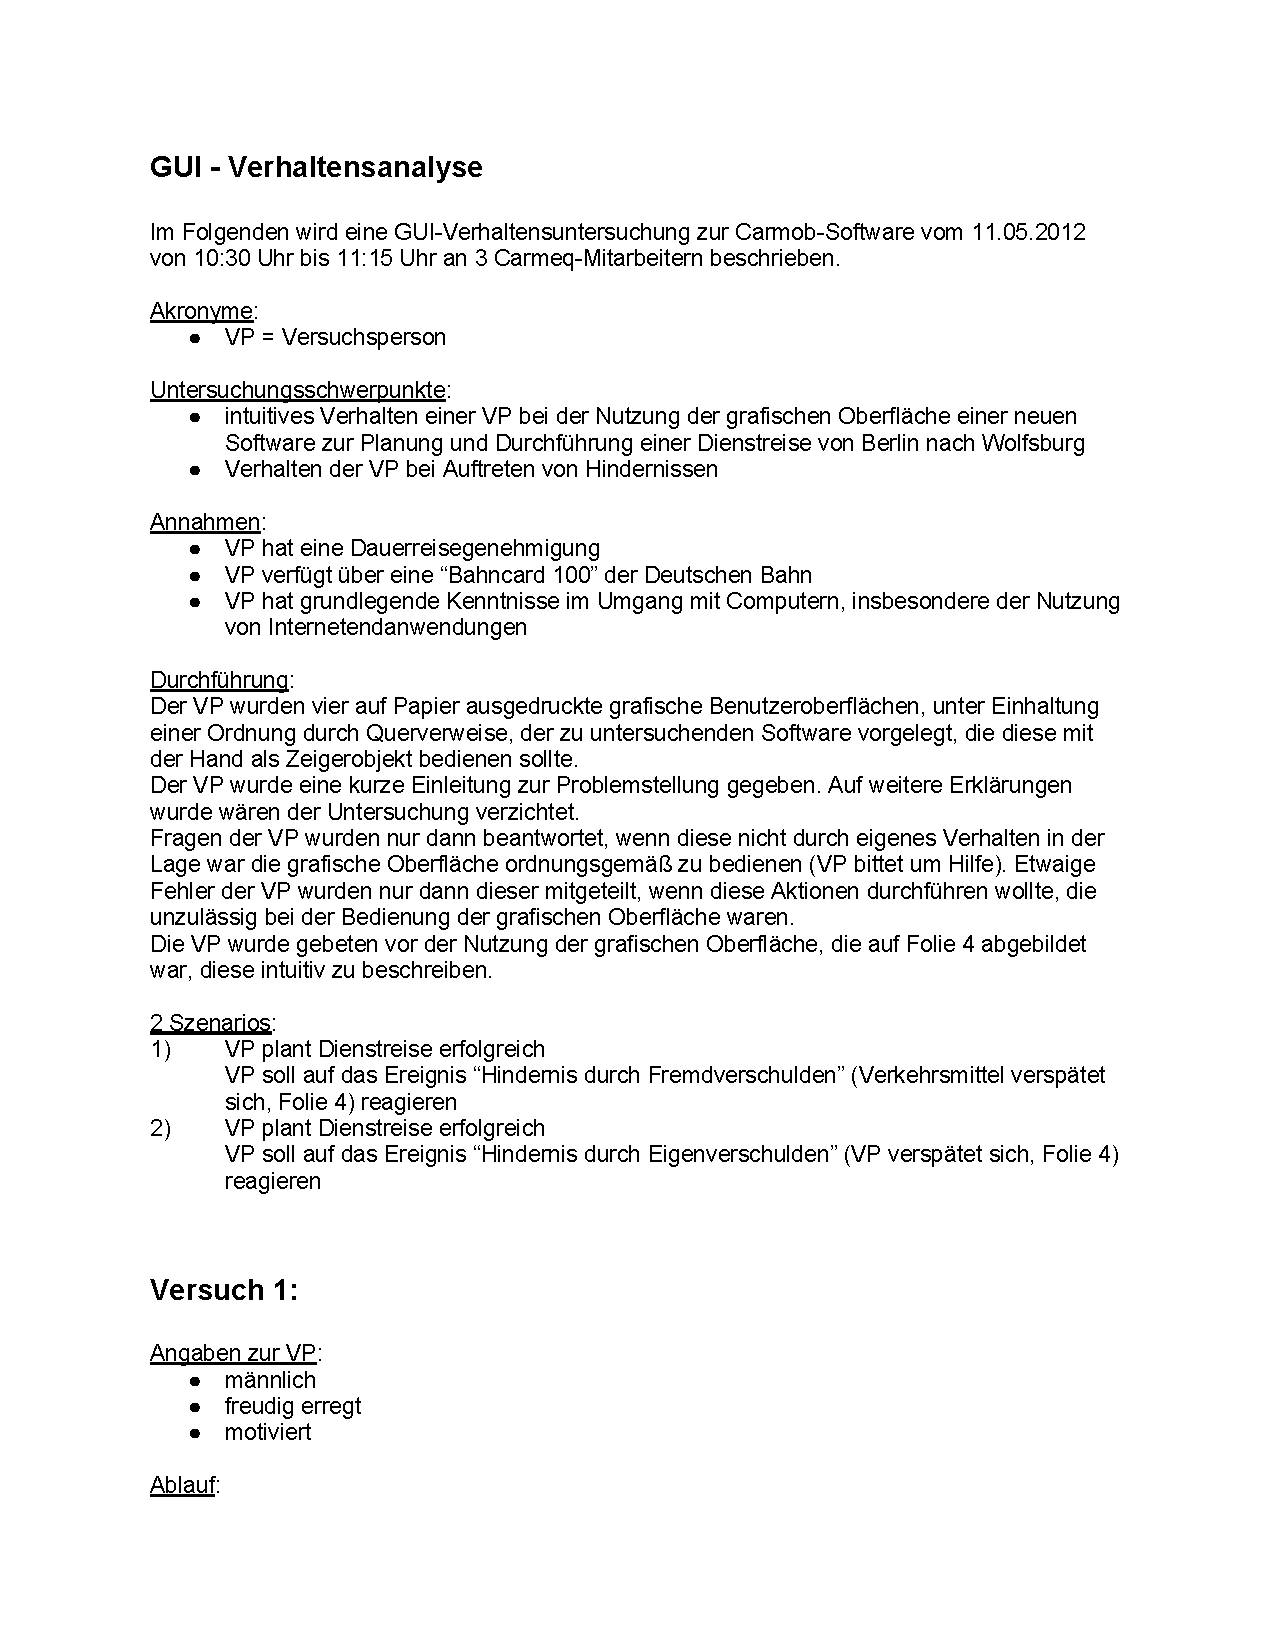
\includepdf[pages=1-6]{07_verhaltensanalyse03.pdf}
\begin{center}
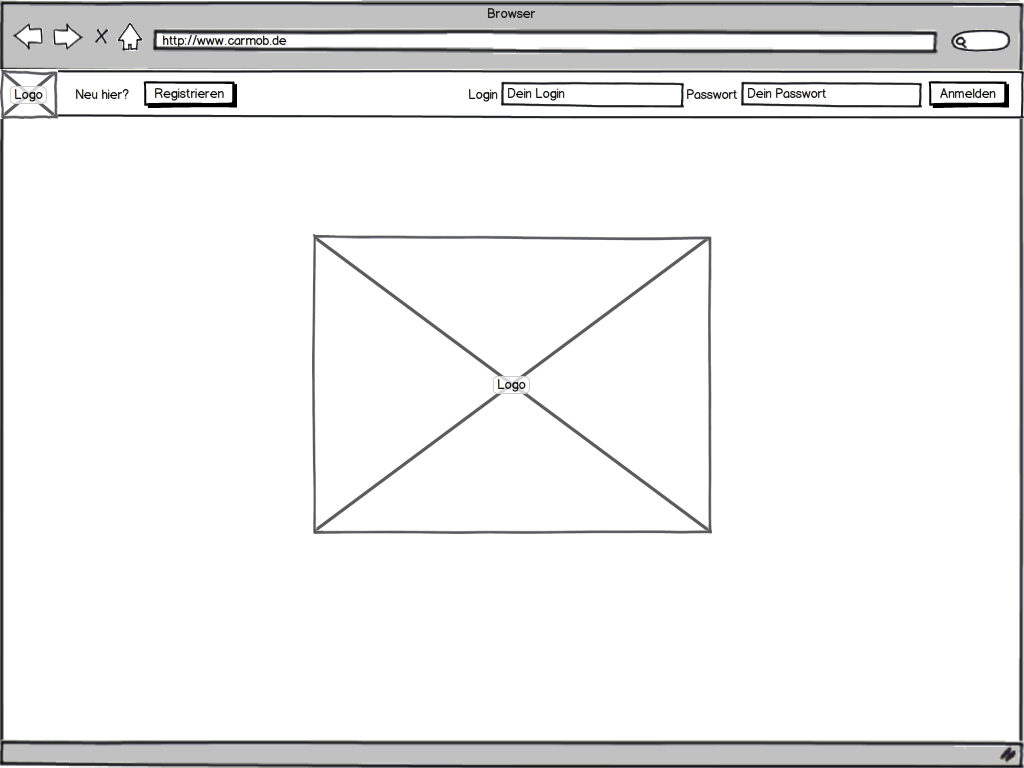
\includegraphics[width=12cm]{08_konvergenter_paperprototyp01_000.png}\\
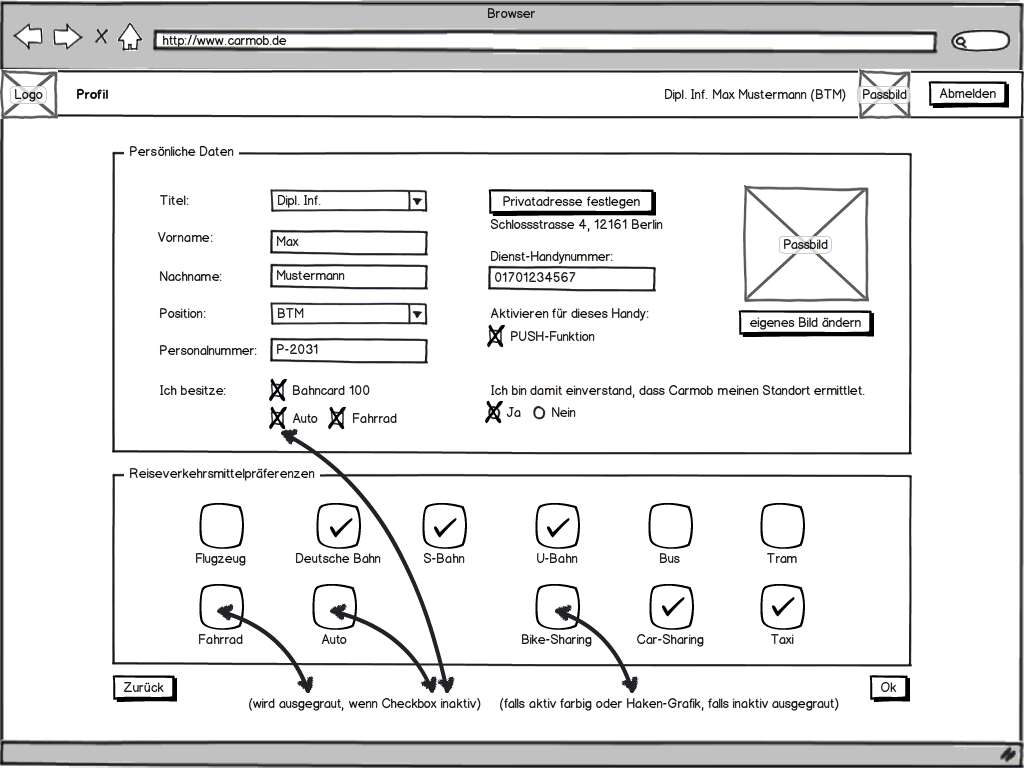
\includegraphics[width=12cm]{08_konvergenter_paperprototyp01_001.png}\\
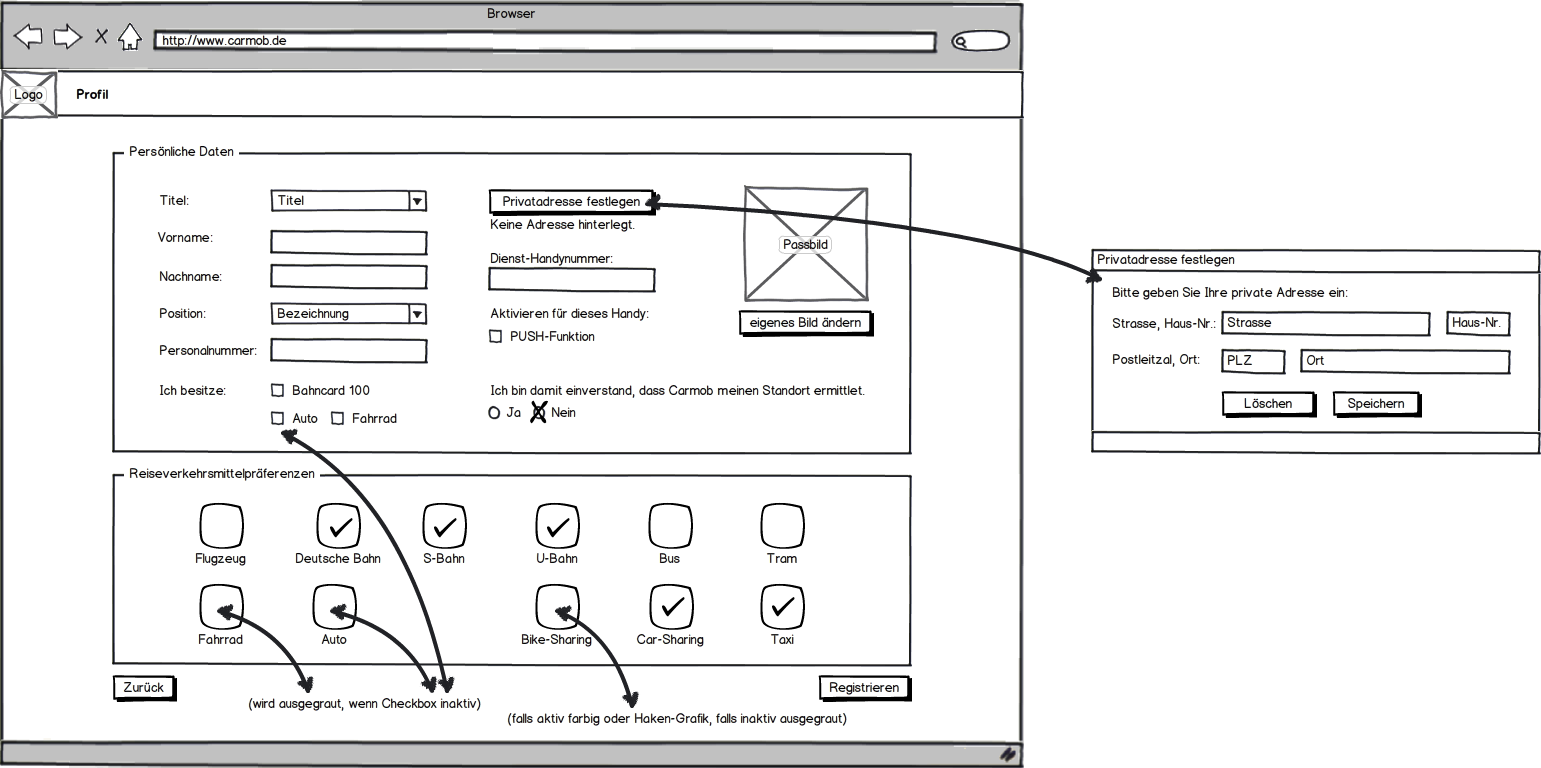
\includegraphics[width=12cm]{08_konvergenter_paperprototyp01_002.png}\\
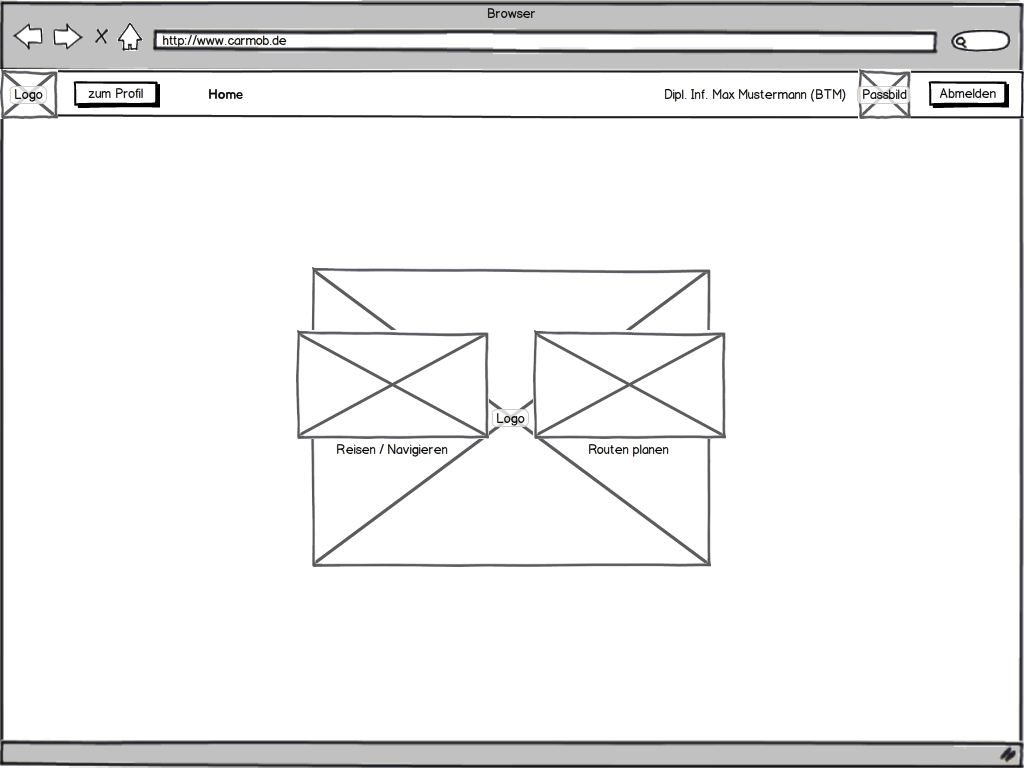
\includegraphics[width=12cm]{08_konvergenter_paperprototyp01_003.png}\\
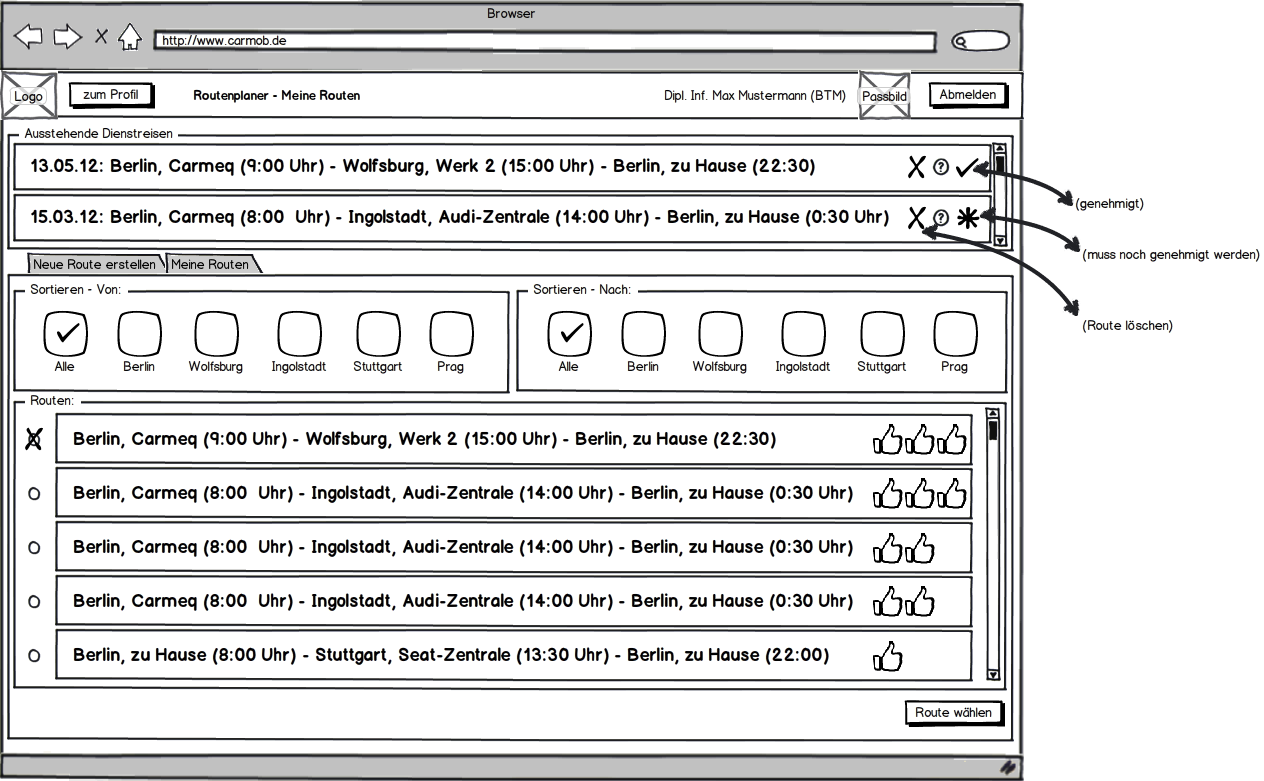
\includegraphics[width=12cm]{08_konvergenter_paperprototyp01_004.png}\\
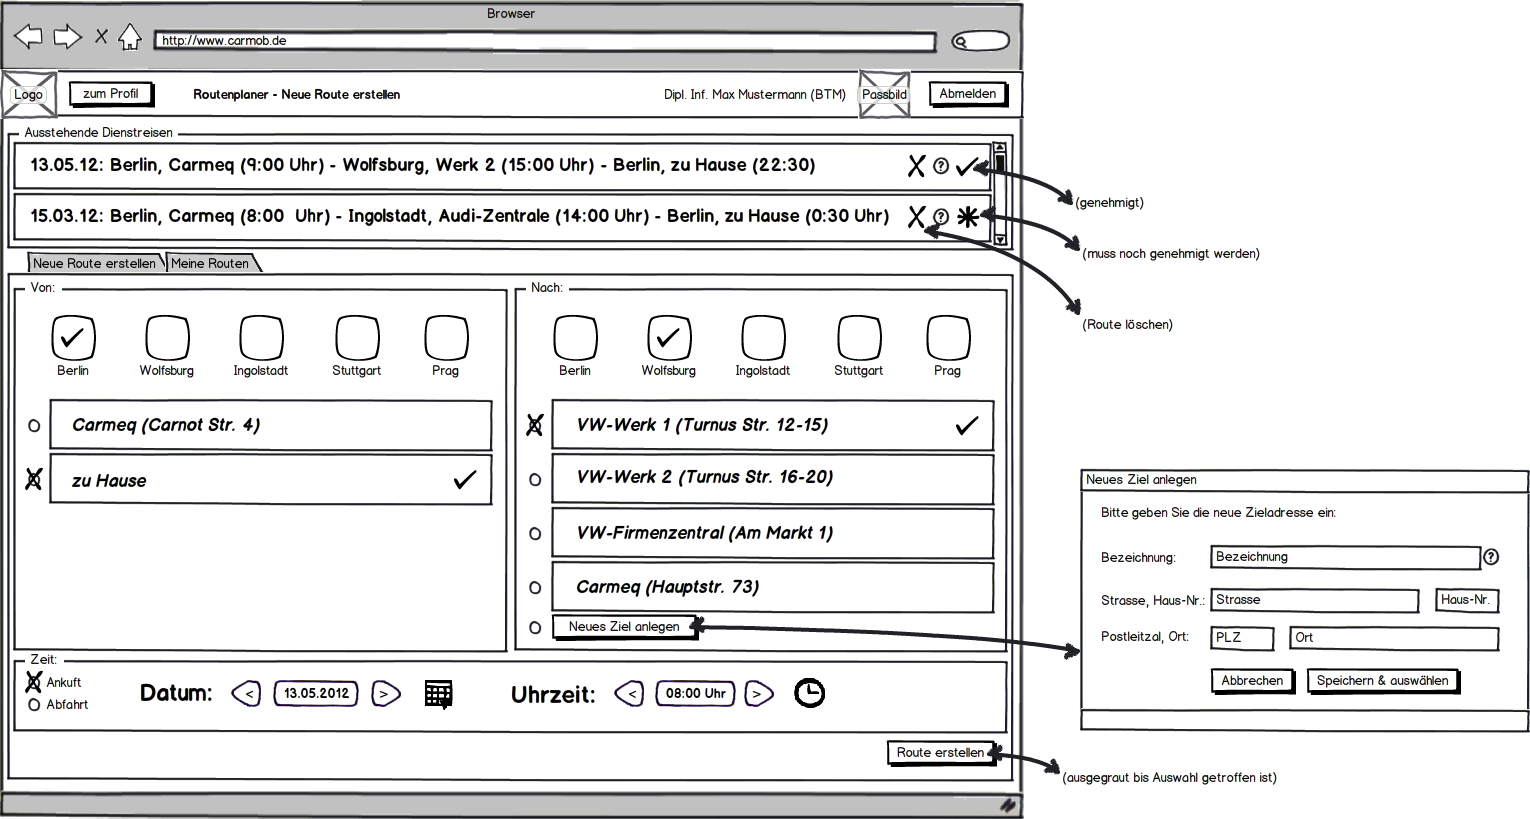
\includegraphics[width=12cm]{08_konvergenter_paperprototyp01_005.png}\\
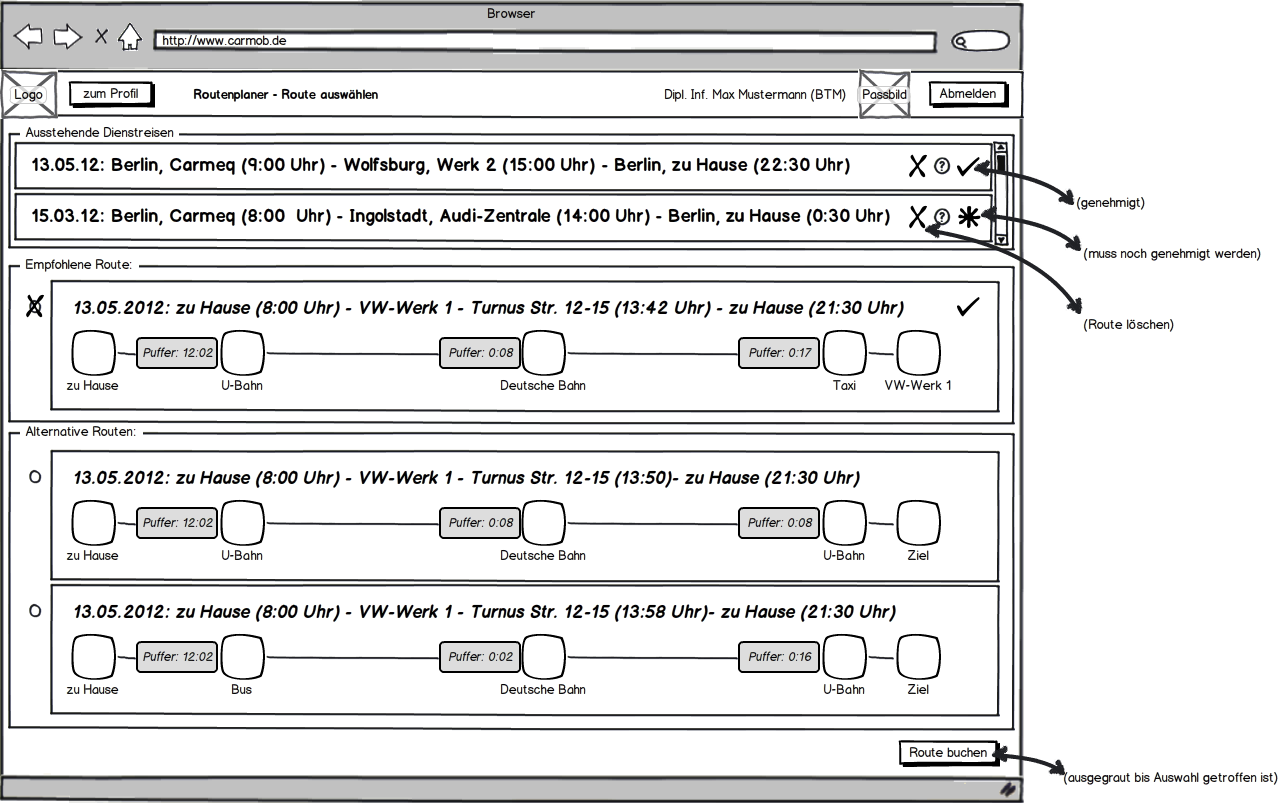
\includegraphics[width=12cm]{08_konvergenter_paperprototyp01_006.png}\\
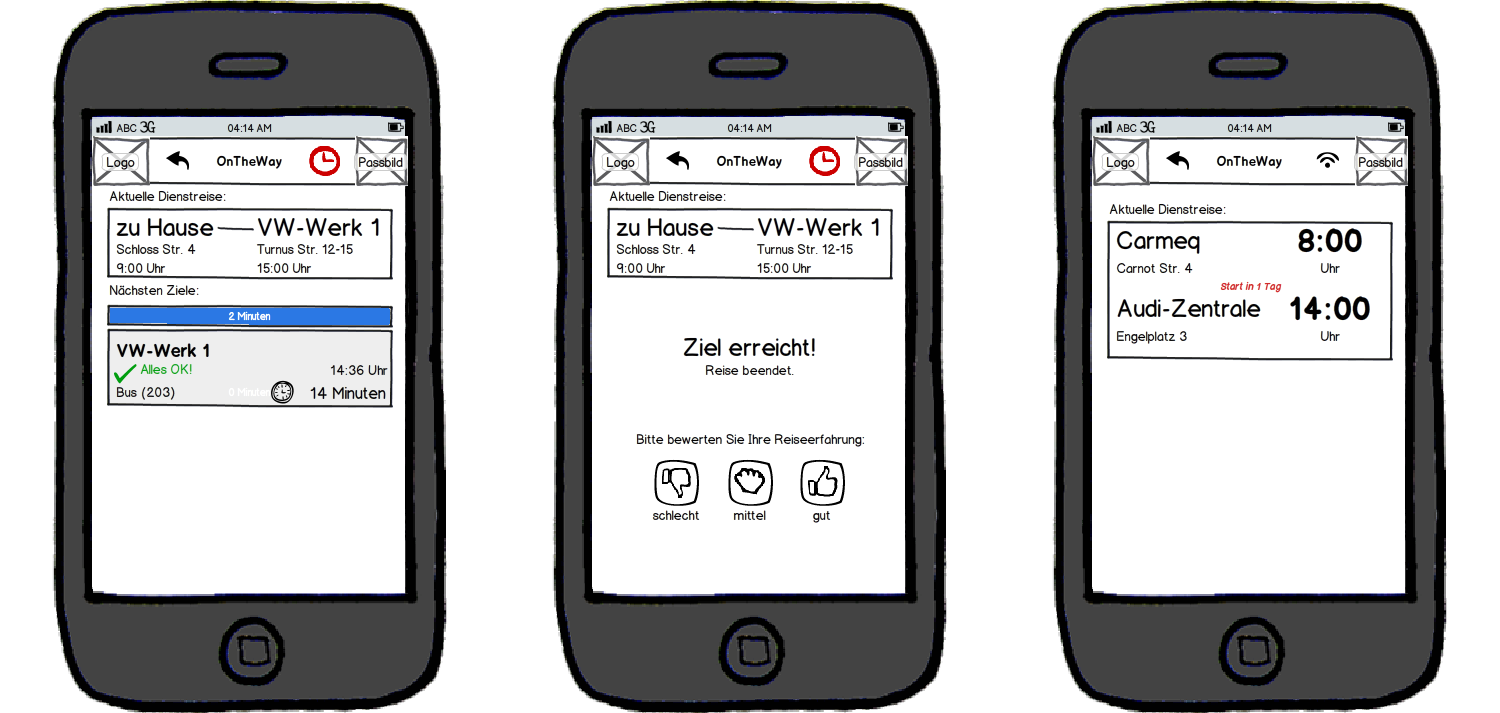
\includegraphics[width=12cm]{08_konvergenter_paperprototyp01_007.png}\\
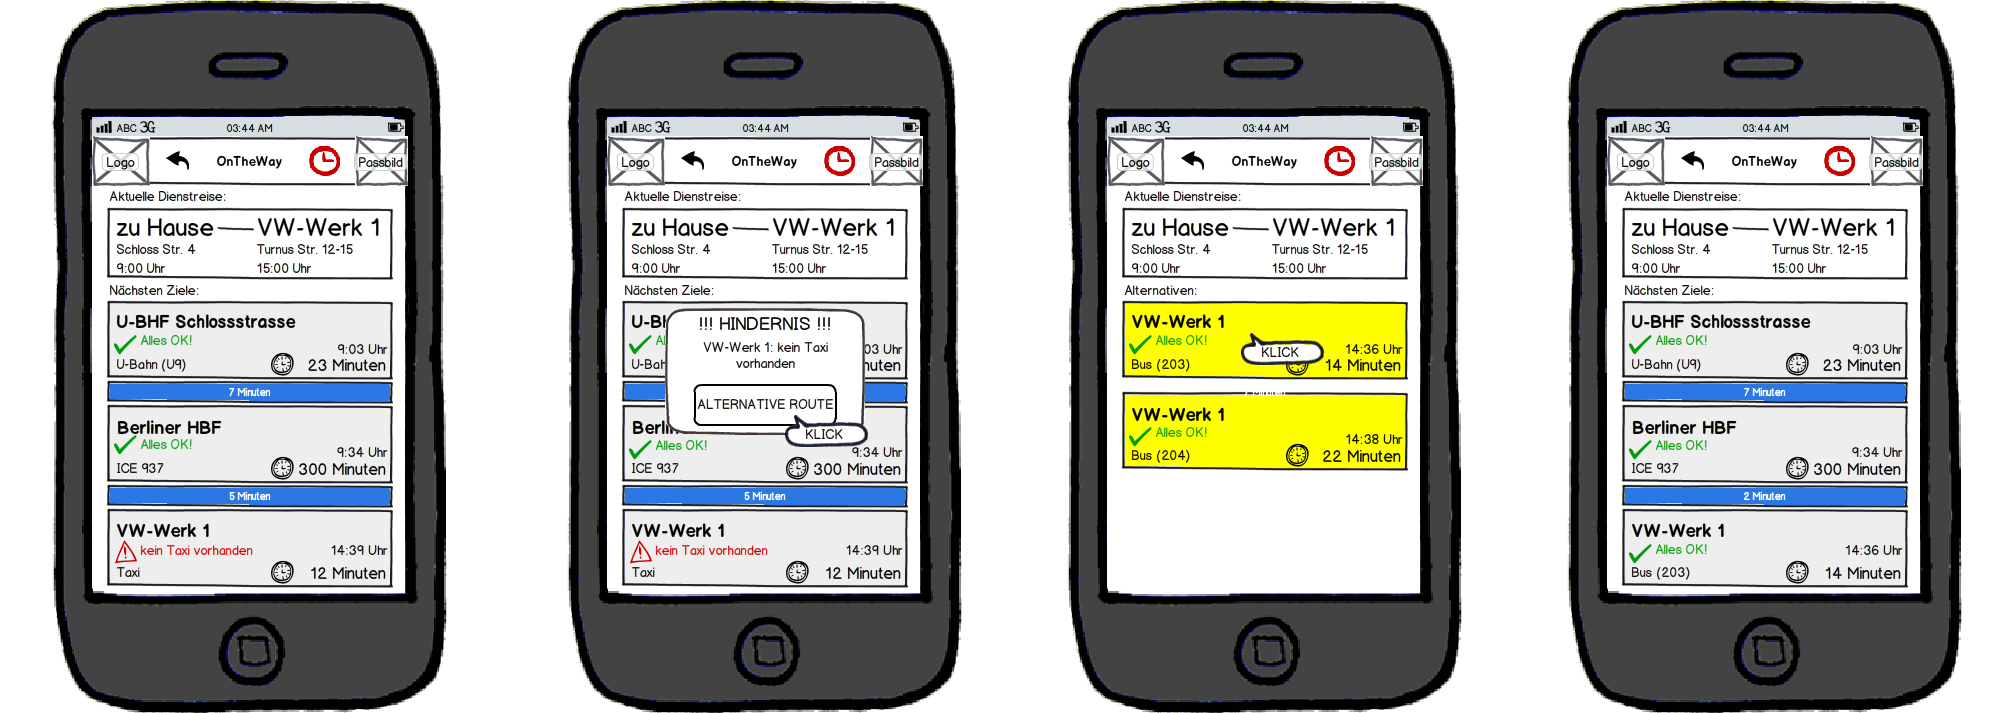
\includegraphics[width=12cm]{08_konvergenter_paperprototyp01_008.png}\\
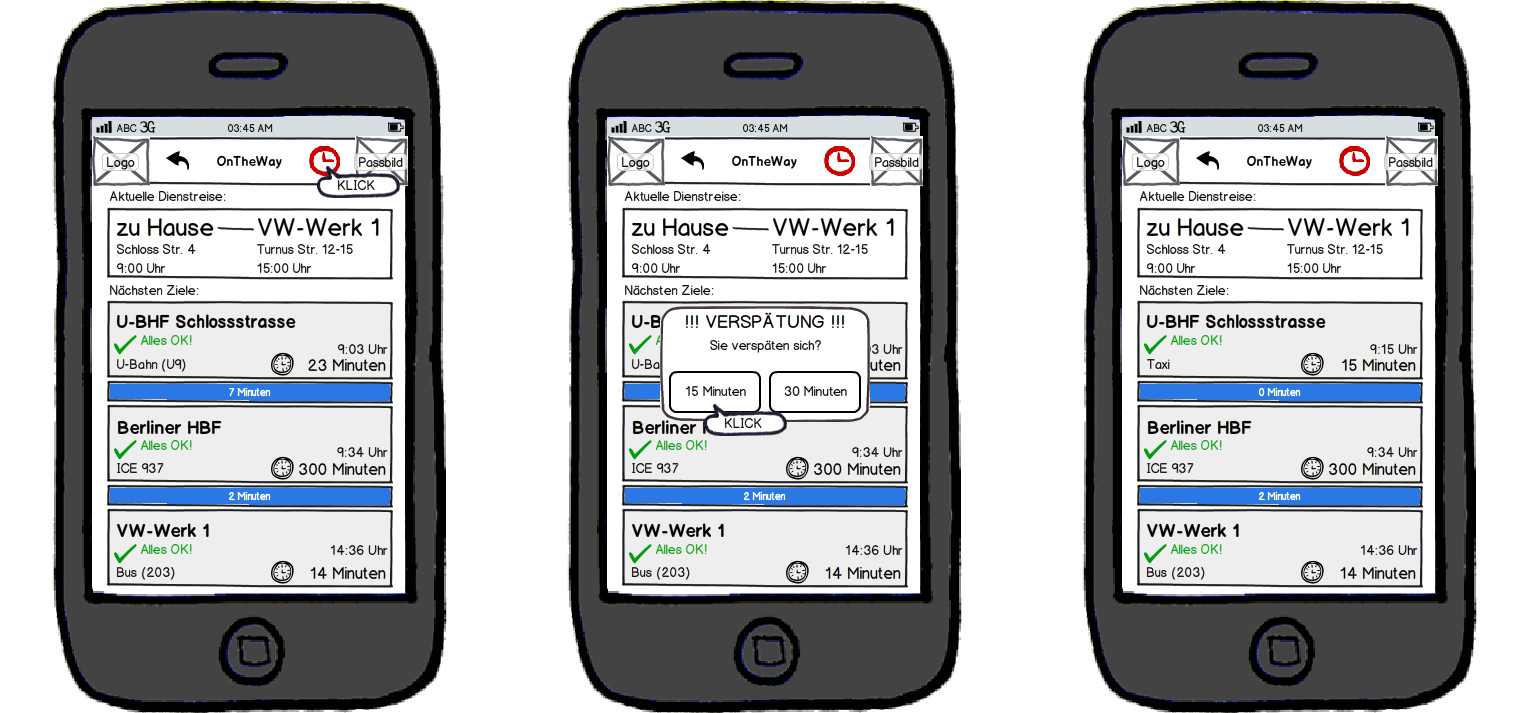
\includegraphics[width=12cm]{08_konvergenter_paperprototyp01_009.png}\\
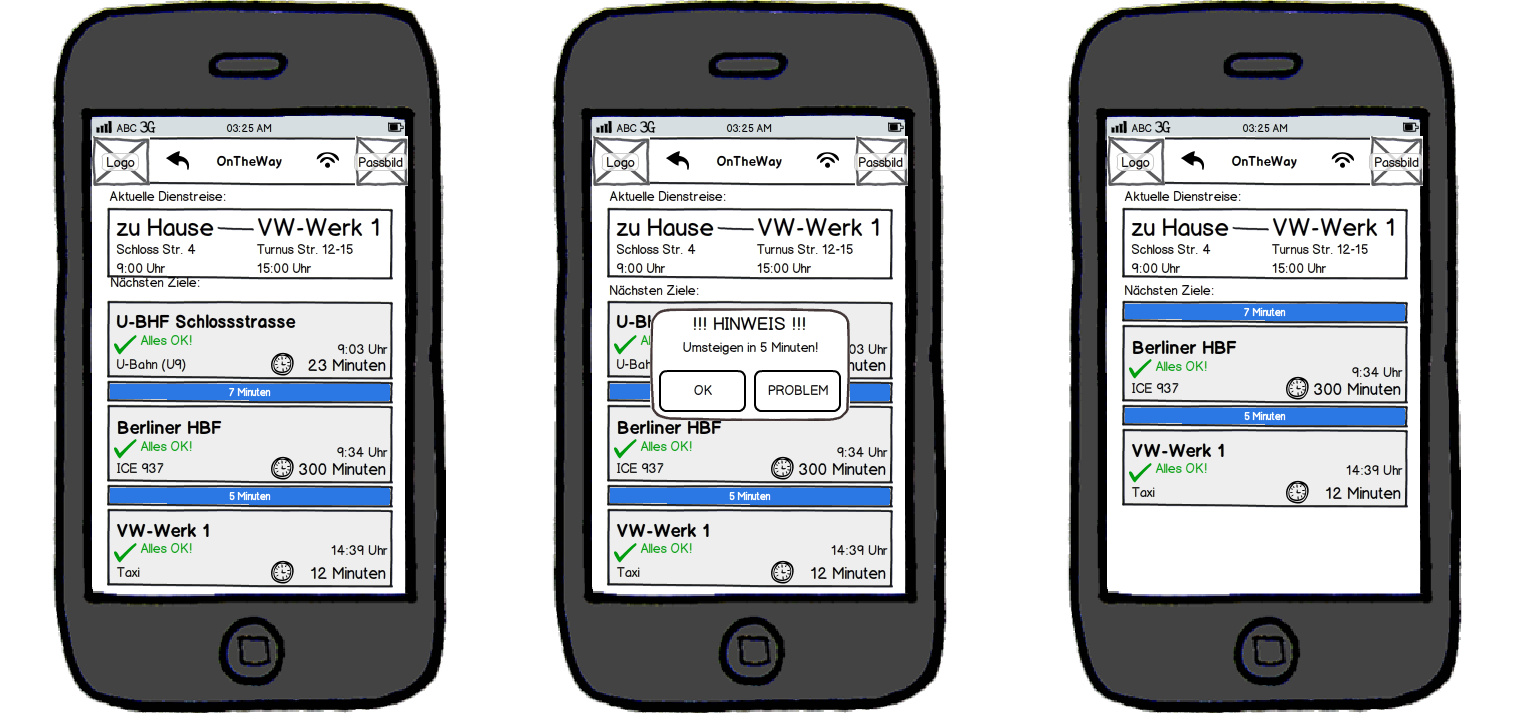
\includegraphics[width=12cm]{08_konvergenter_paperprototyp01_010.png}\\
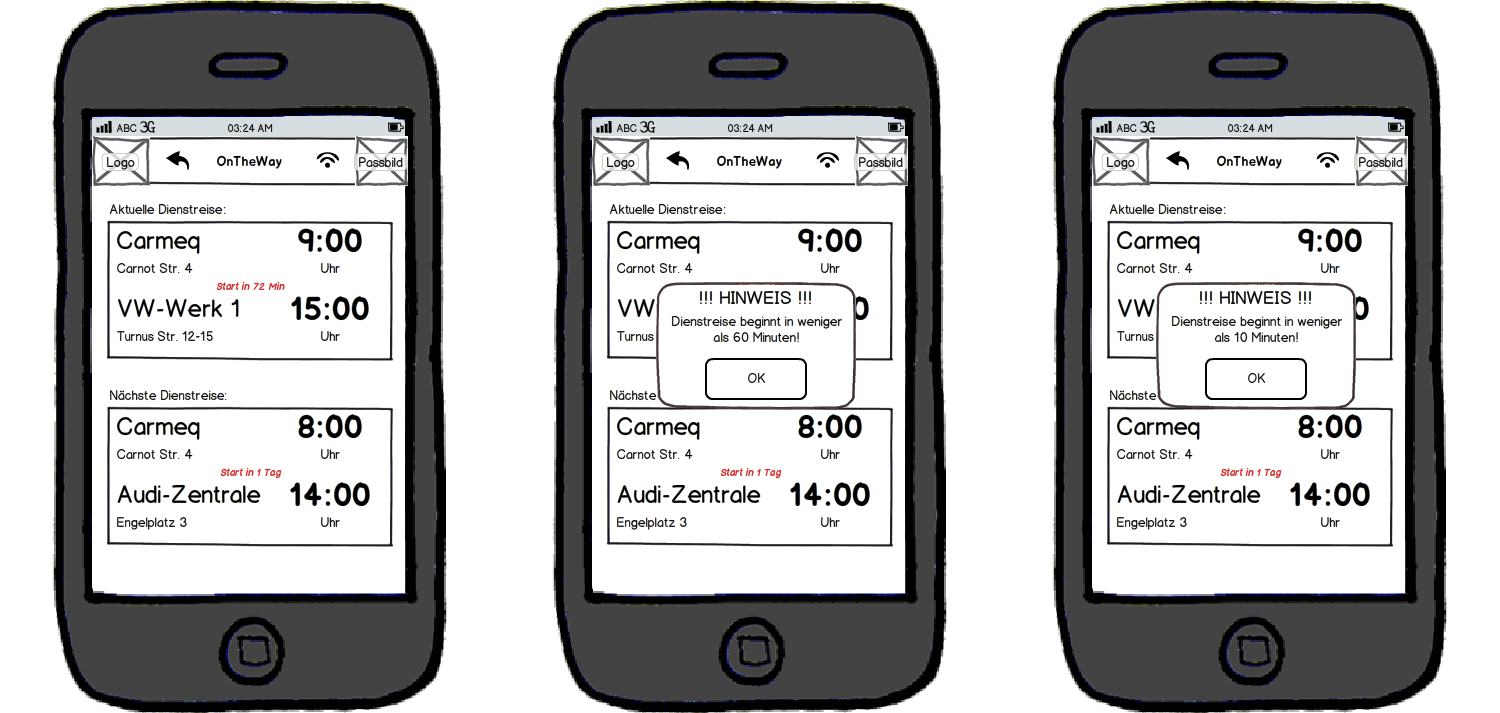
\includegraphics[width=12cm]{08_konvergenter_paperprototyp01_011.png}\\
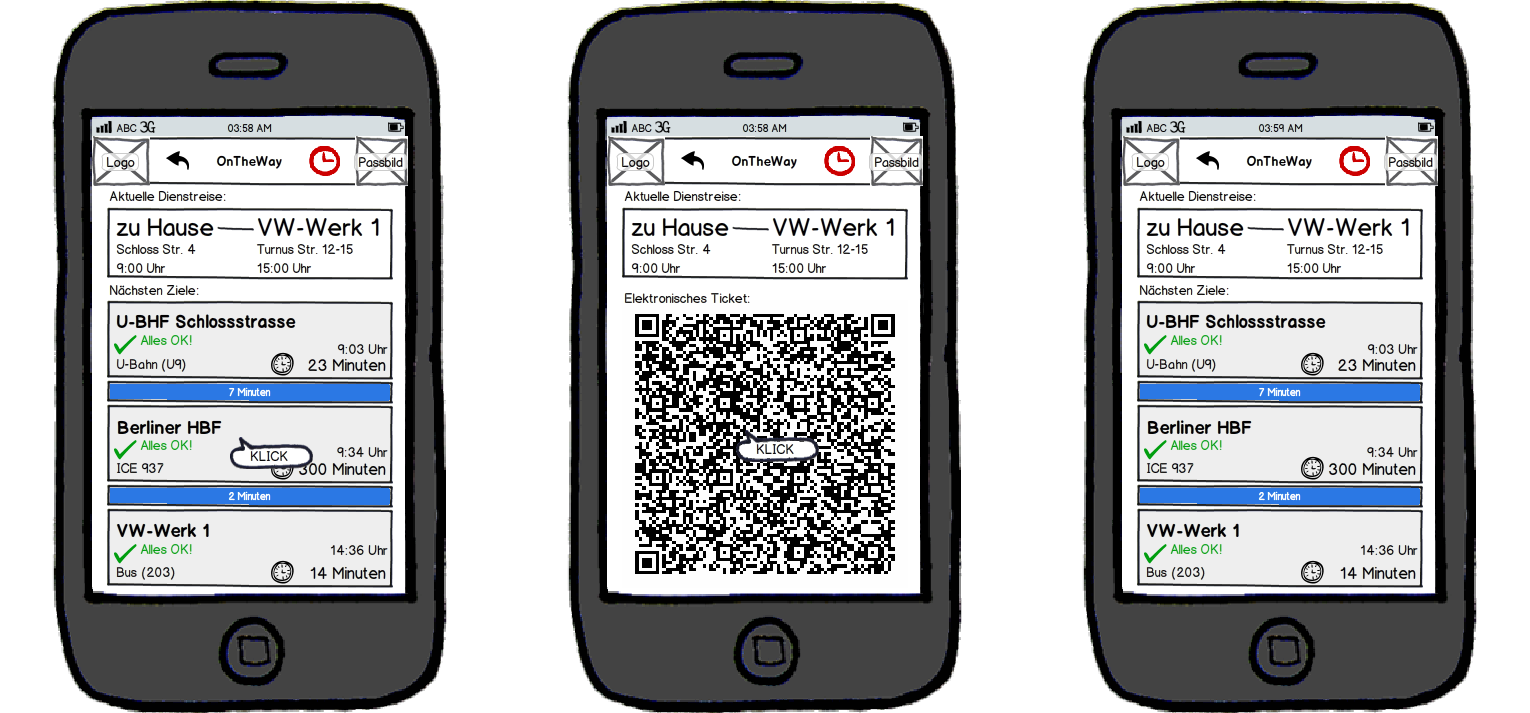
\includegraphics[width=12cm]{08_konvergenter_paperprototyp01_012.png}
\end{center}
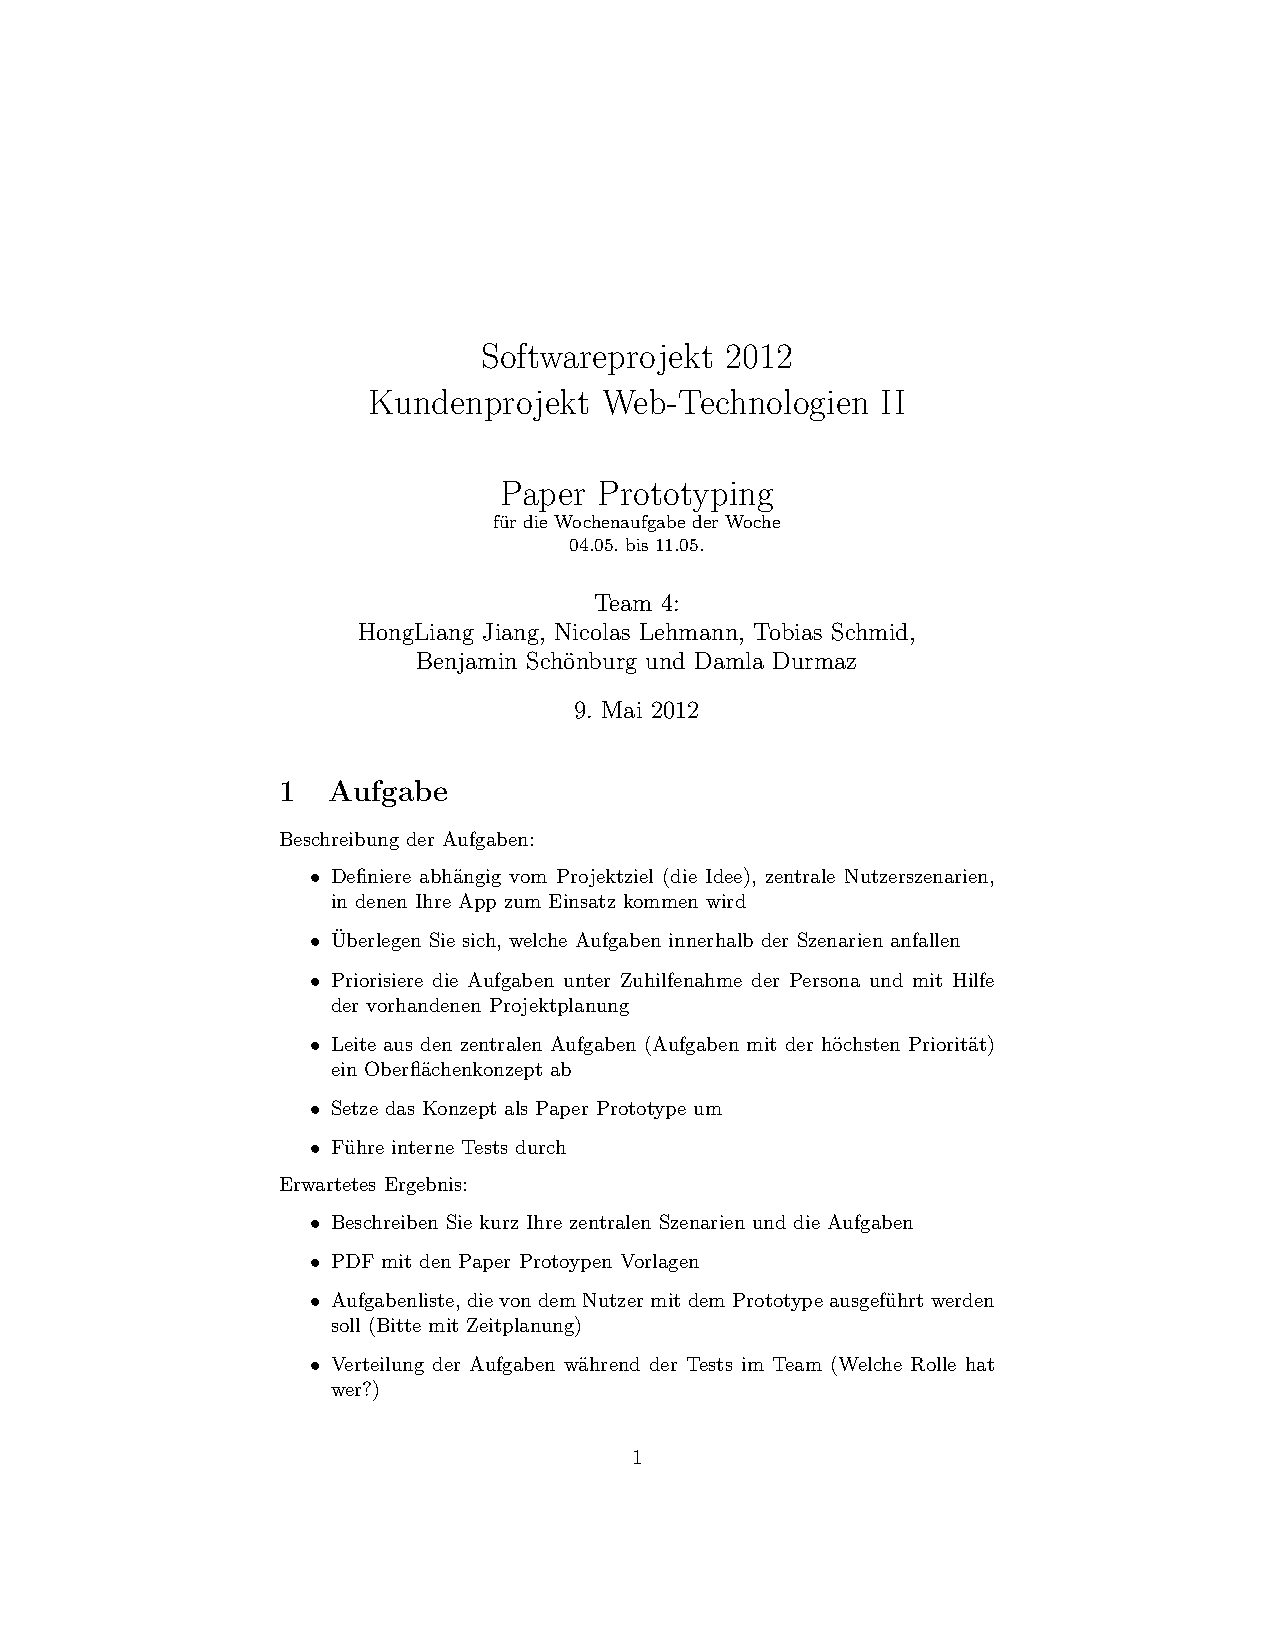
\includepdf[pages=1-13]{09_userstories_szenarien01.pdf}
\includepdf[pages=1-13]{09_userstories_szenarien02.pdf}
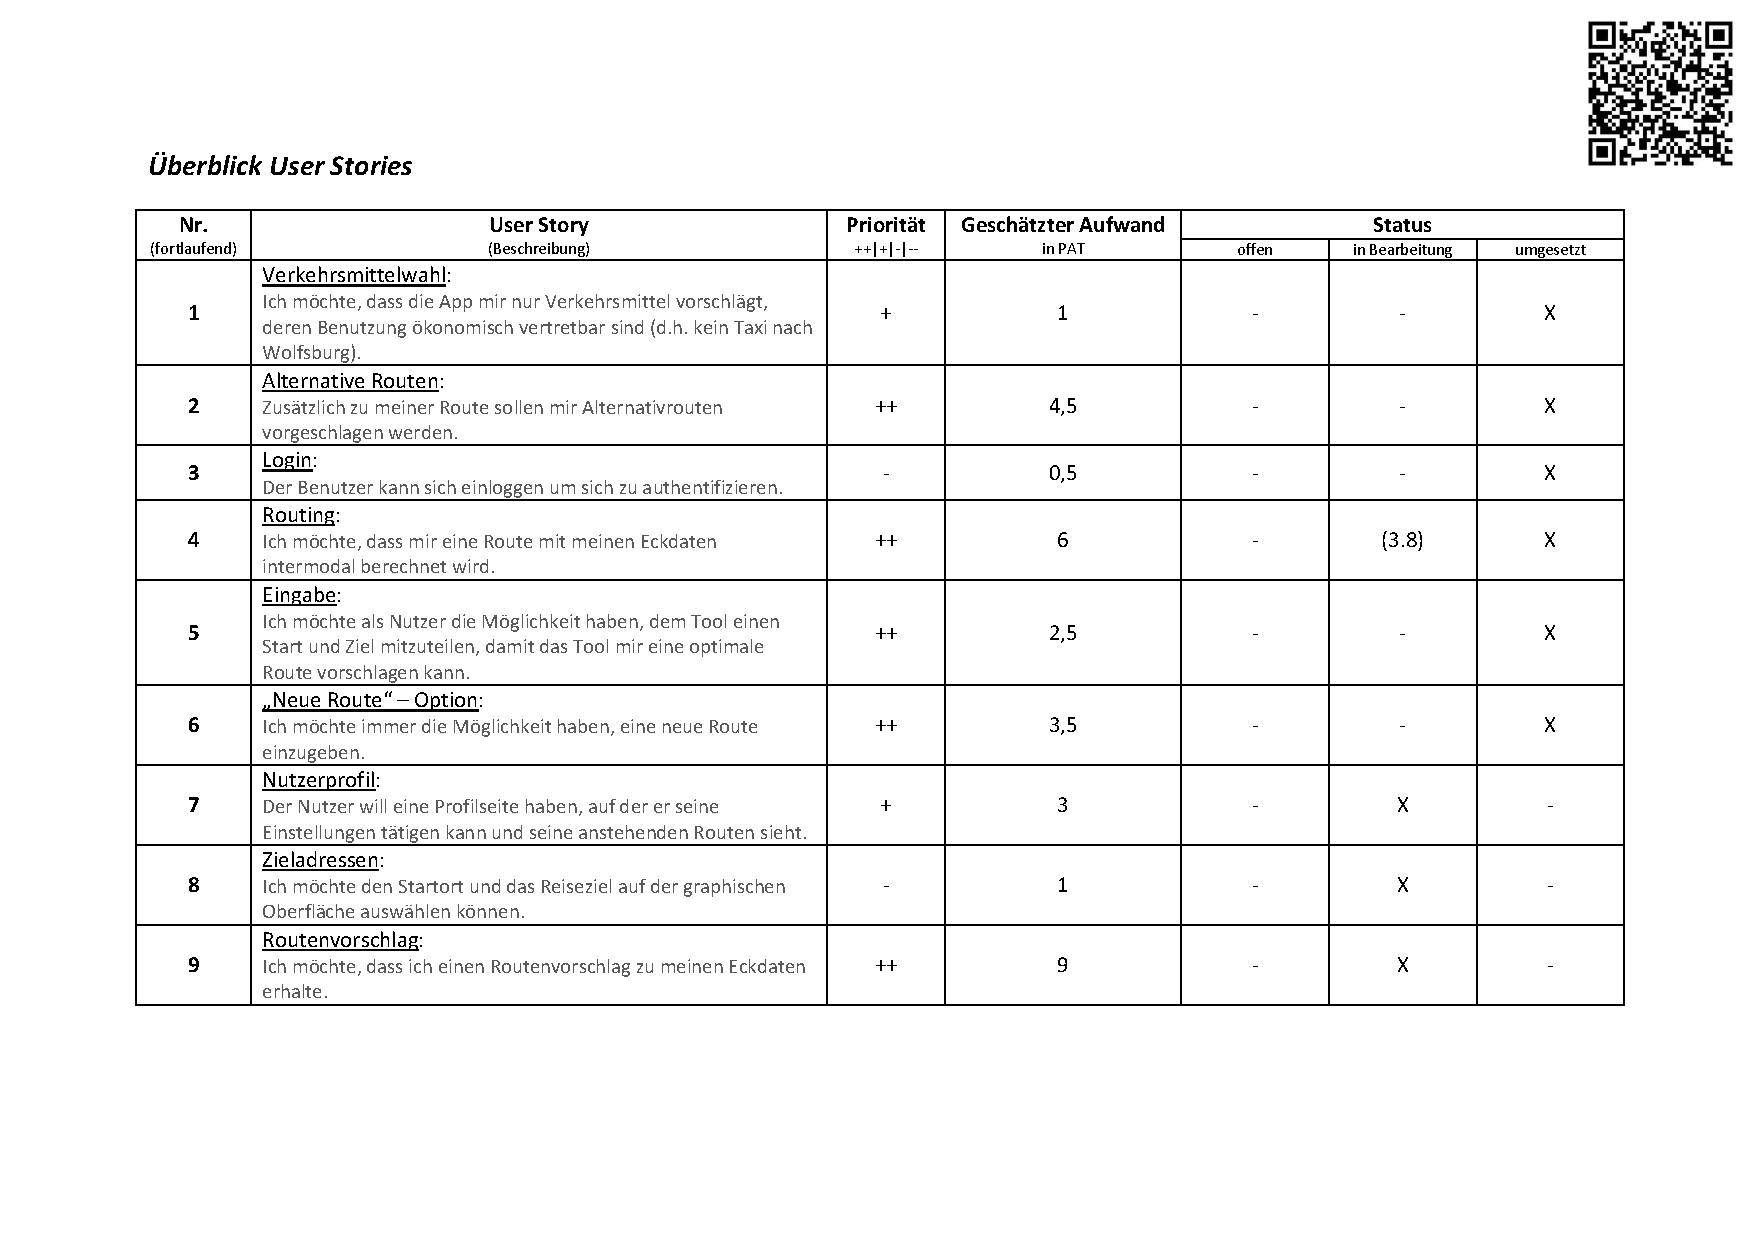
\includepdf[pages=1-3]{00_iterationsplanung03.pdf}
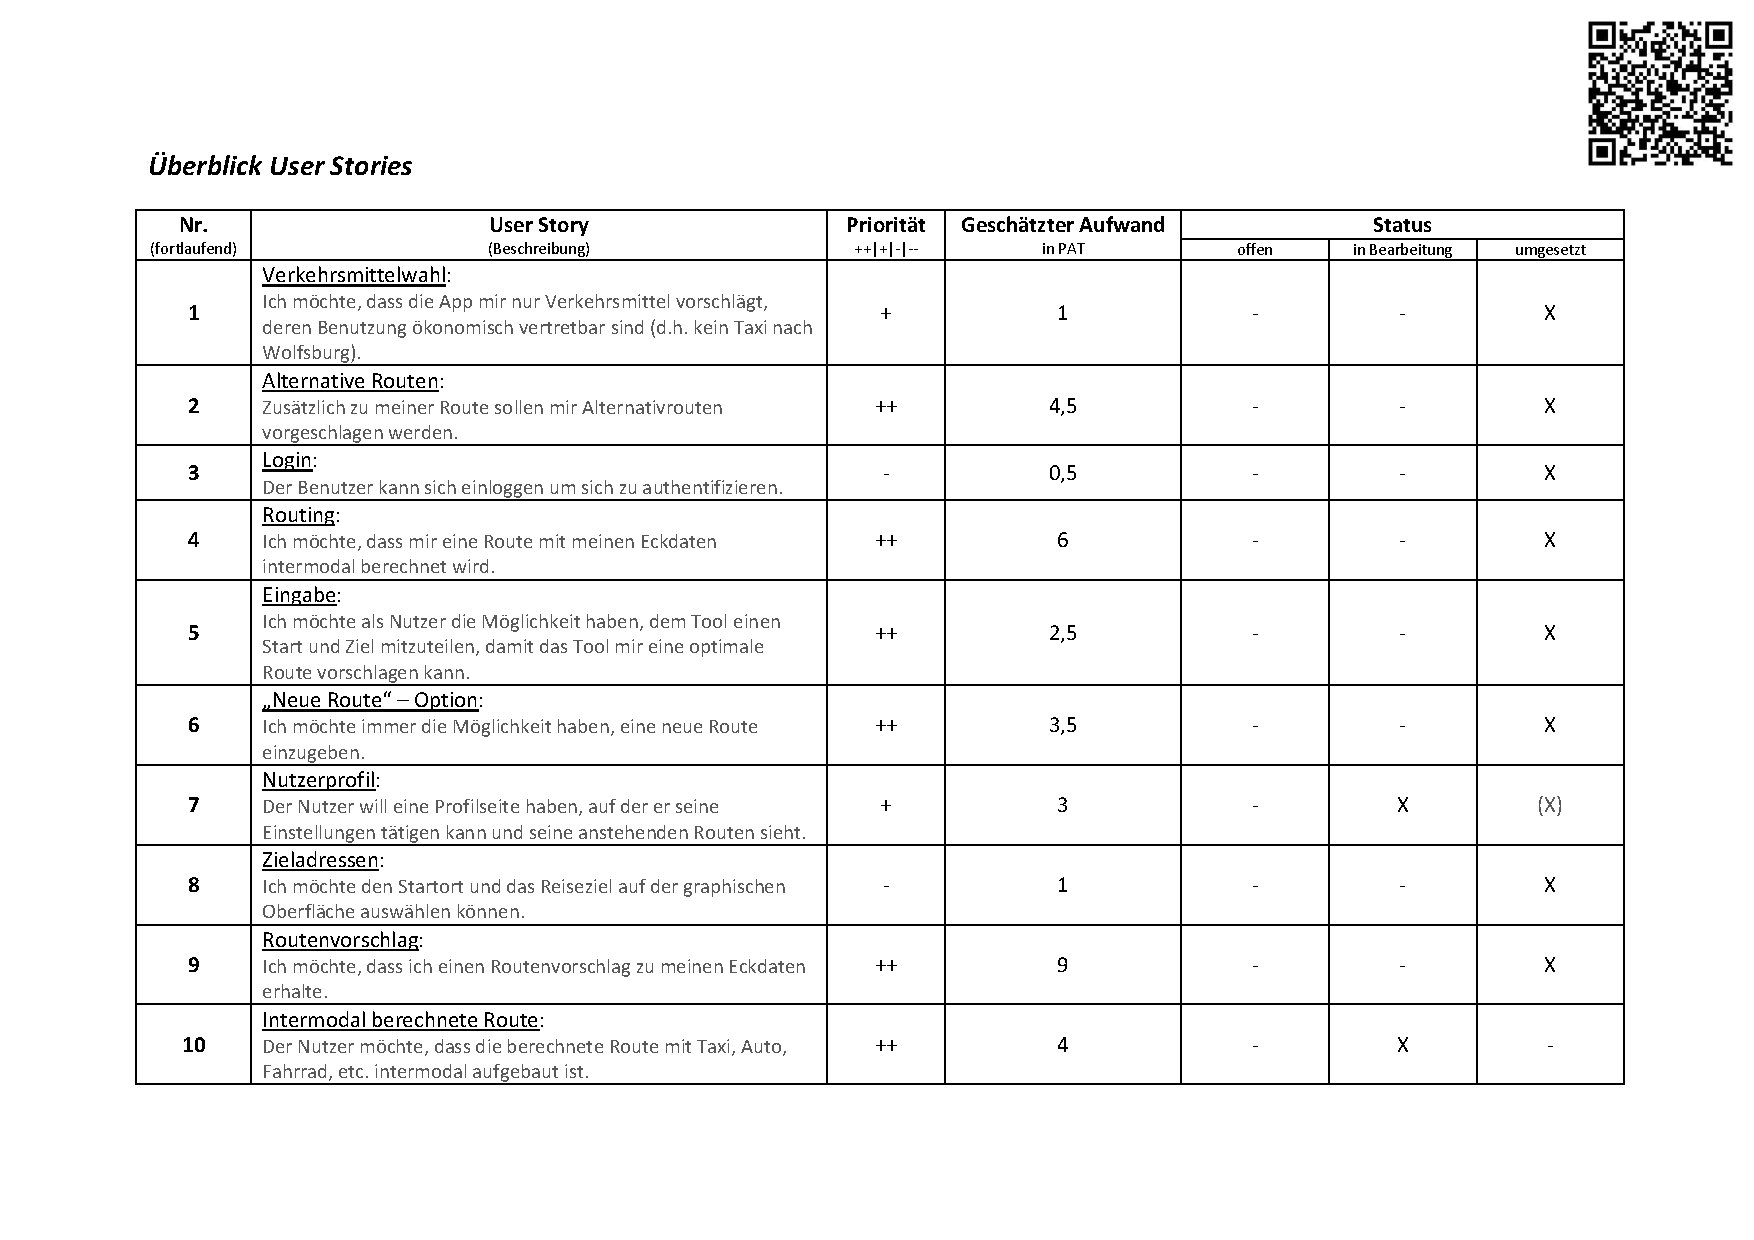
\includepdf[pages=1-5]{00_iterationsplanung04.pdf}
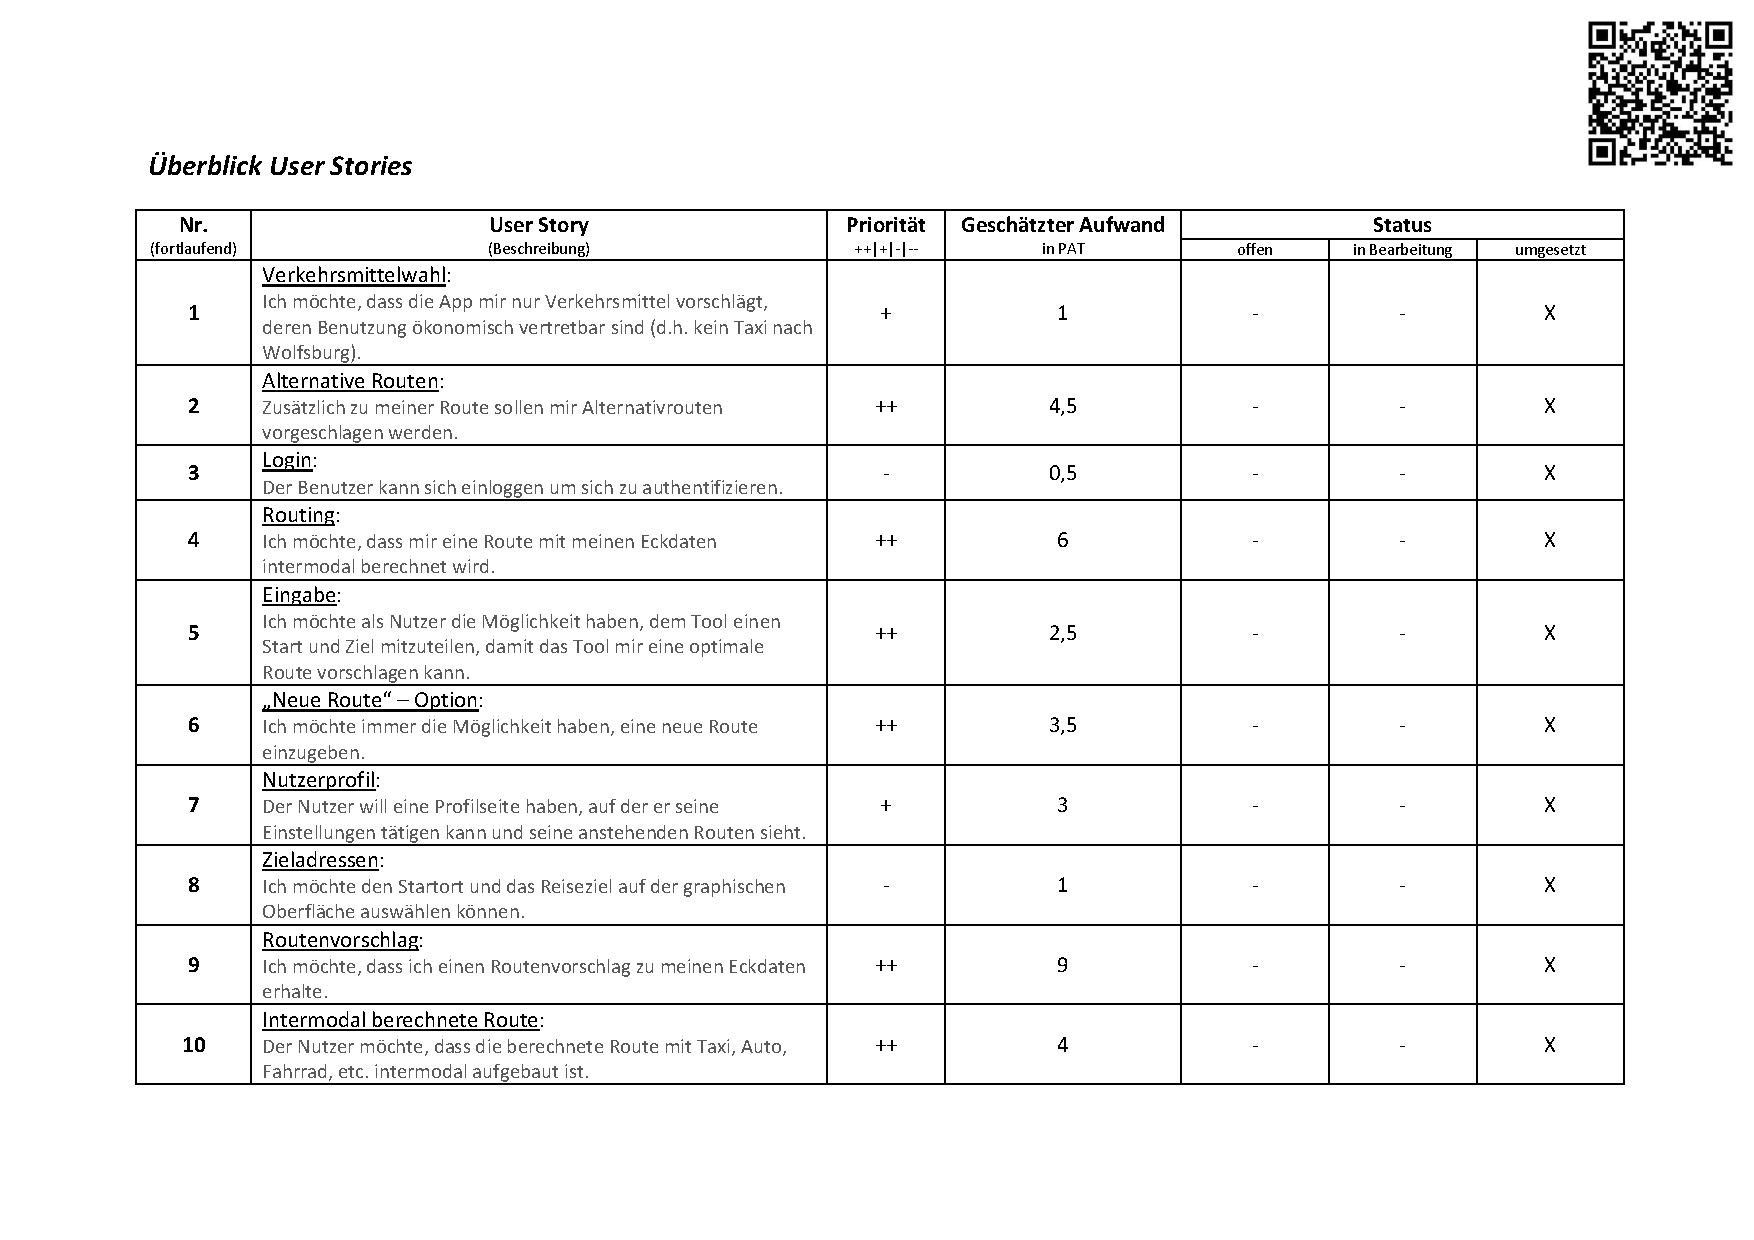
\includepdf[pages=1-6]{00_iterationsplanung05.pdf}

\section{Phase: Rekonzeption und 1. Iteration}

In dieser Phase sollten aus den Papier-Prototypen UserStories abgeleitet und implementiert werden. Zus\"atzlich sollte der Umsetzungsaufwand gesch\"atzt und schriftlich festgehalten werden, um die organisatorische Planung einer Iterationsphase zu erlernen. Da wir die Rekonzeptionierung erst abschlie\ss en mussten konnten wir erst relativ sp\"at mit der Planung der Iterationsphase und der Implementierung beginnen.

\subsection{Woche 05: Szenarien, Anwendungsf\"alle}

\subsubsection{Was hat das Team getan?}

Wir haben den Paper-Prototyp mit 10 Mitarbeitern der Carmeq GmbH getestet und anschlie\ss end ausgewertet. Daraufhin haben wir Anwendungsf\"alle und Szenarien entwickelt und einen neuen, auf den gewonnenen Erkenntnissen aus den Tests basierenden, Paper-Prototyp entwickelt.

\subsubsection{Zentrale Entscheidungen}

Wir haben uns dazu entschieden mit deutlich mehr Mitarbeitern die Paper-Prototypen zu testen um einen neuen genaueren und somit besseren Paper-Prototype entwickeln zu k\"onnen. Aufgrund dessen hat das Team zus\"atzliche Test mit Mitarbeitern der Carmeq GmbH durchgef\"uhrt.

\subsection{Woche 06: Implementierung eines Grundger\"usts}

\subsubsection{Was hat das Team getan?}

Wir haben ein Grundger\"ust f\"ur unsere Software entworfen und ein ERDD dieser erstellt. Erste Grundfunktionalit\"aten und ein Login wurden programmiert.

\subsubsection{Zentrale Entscheidungen}

Unabh\"angig von den ben\"otigten Entit\"atstypen (Trip, Connection, TransportationMean, Angel, User) haben wir uns f\"ur einen zentral verwaltenden Entit\"atstypen (Tripmanagement) entschieden.

\section*{Ergebnisse dieser Phase}

Wir haben die Papier-Prototypen mehrfach weiterentwickelt bis wir einen finalen \textit{konvergenten Papier-Prototypen} erzeugen konnten den wir als Basis f\"ur die \textit{Implementierung des Grundger\"ust unserer Softwarel\"osung} verwendet haben. Wir haben ein ERDD f\"ur das Datenmodell erzeugt.

\begin{itemize}
\item finaler Paper-Prototype (PNG)
\item Datenmodelle erstellt (Quellcode)
\item ERDD erstellt (PNG)
\end{itemize}

\begin{center}
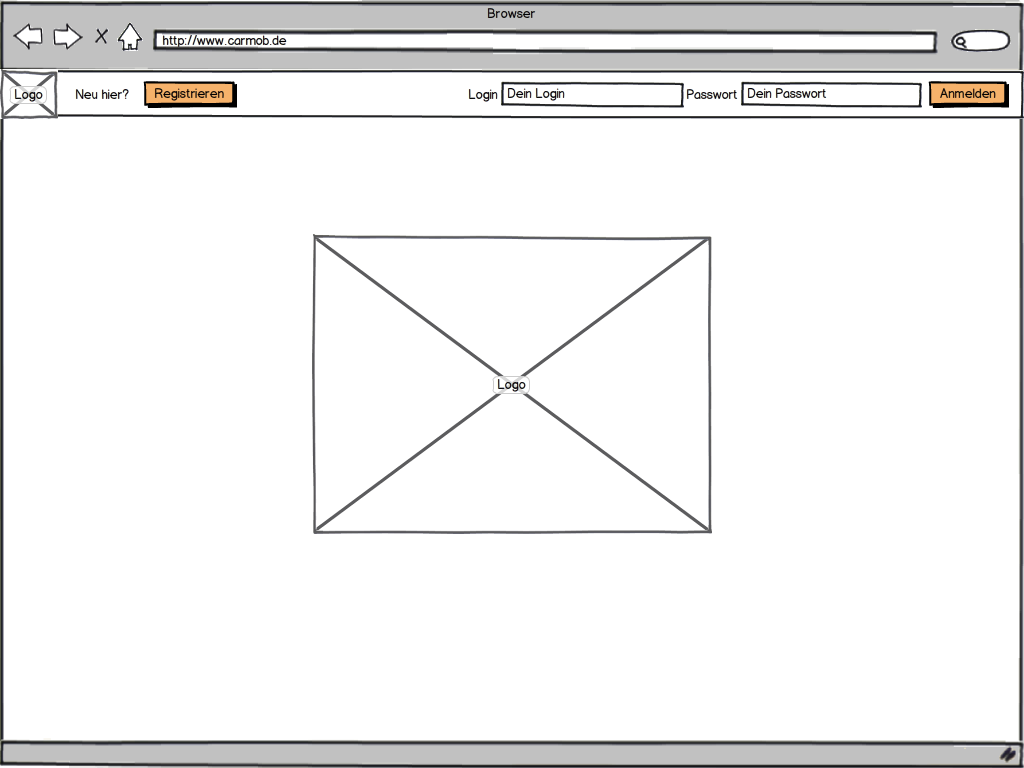
\includegraphics[width=12cm]{10_finaler_paperprototyp_001.png}\\
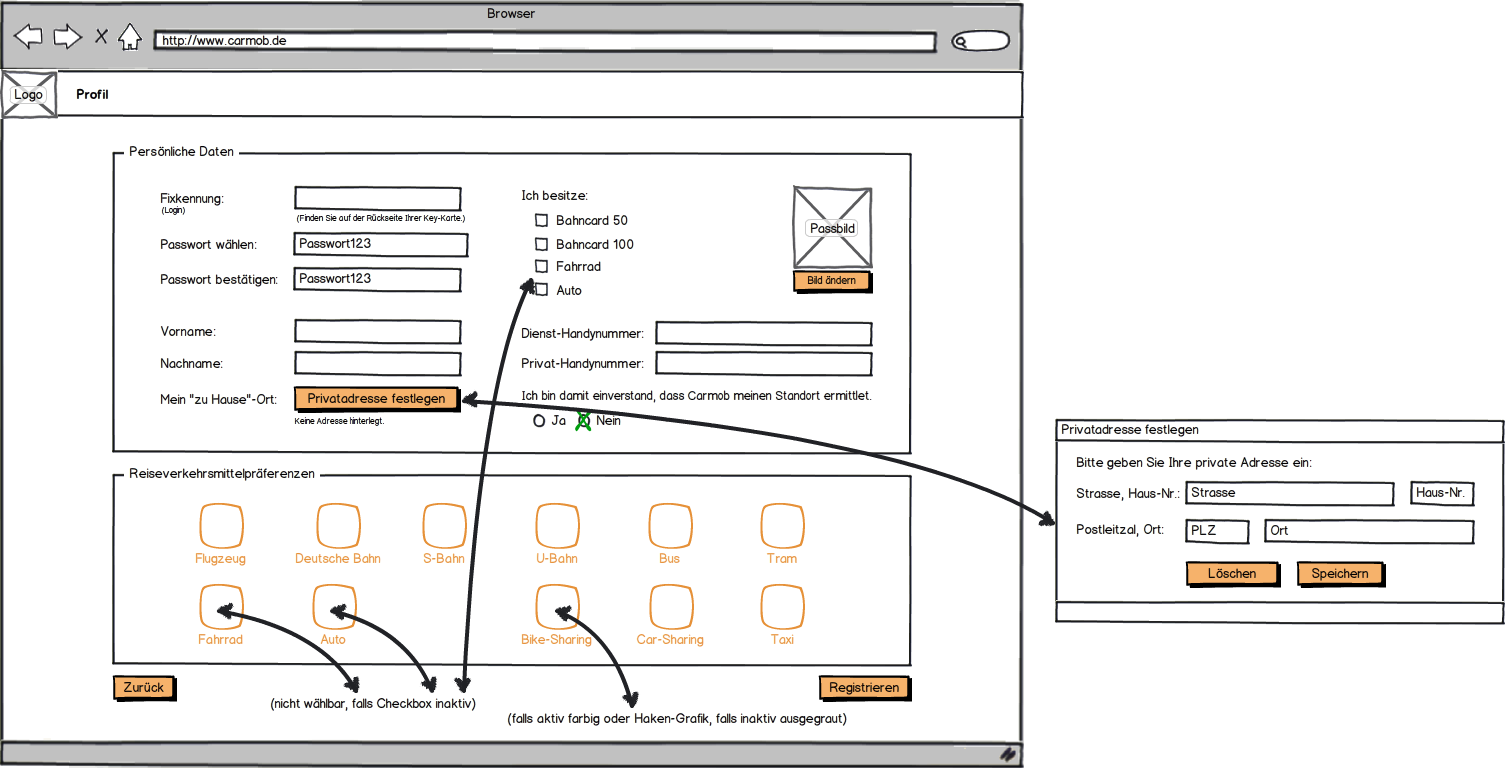
\includegraphics[width=12cm]{10_finaler_paperprototyp_002.png}\\
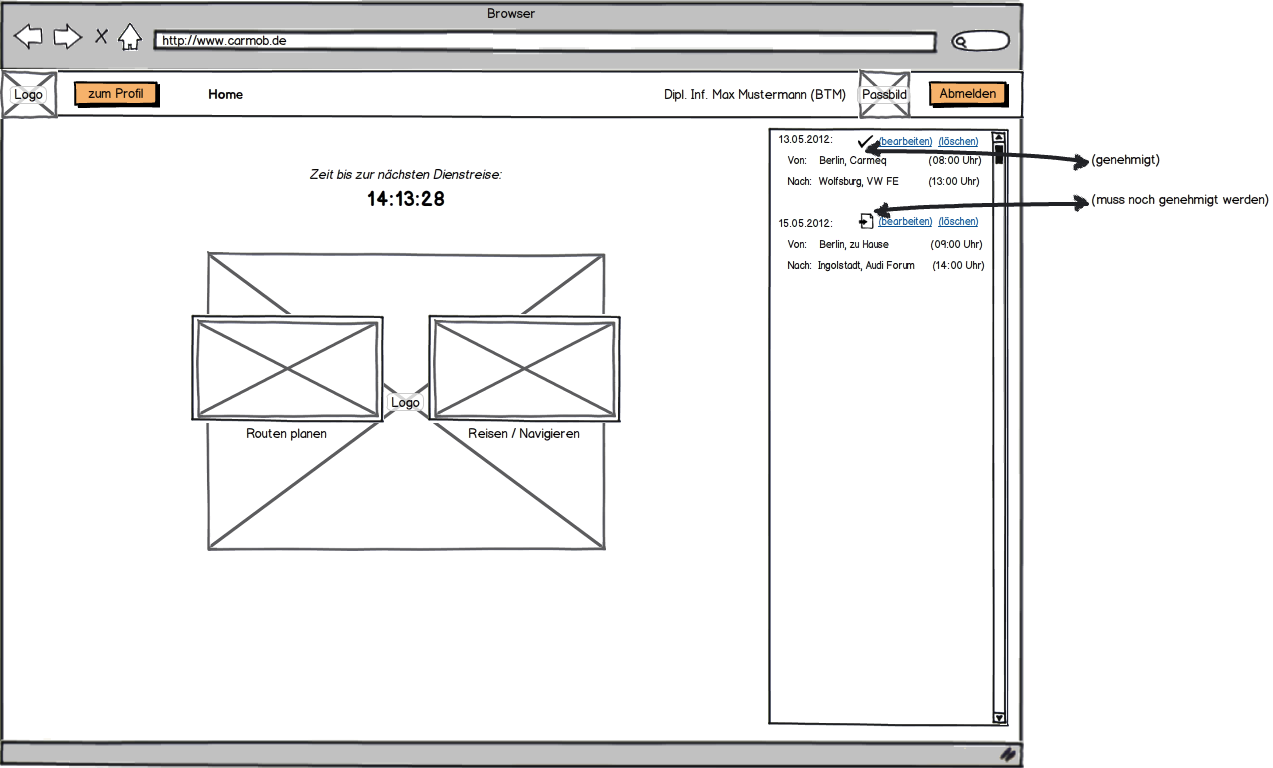
\includegraphics[width=12cm]{10_finaler_paperprototyp_003.png}\\
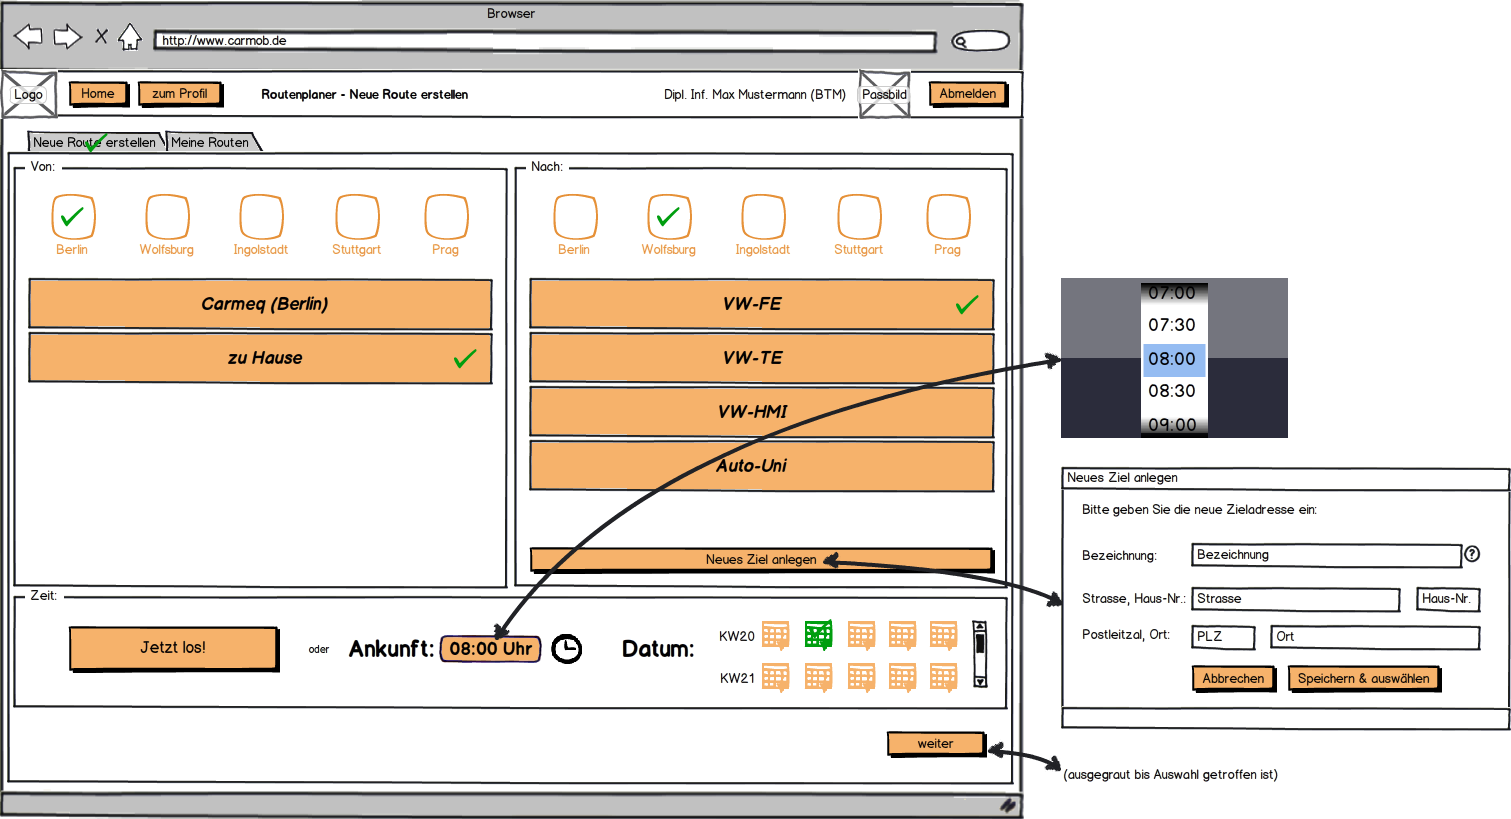
\includegraphics[width=12cm]{10_finaler_paperprototyp_004.png}\\
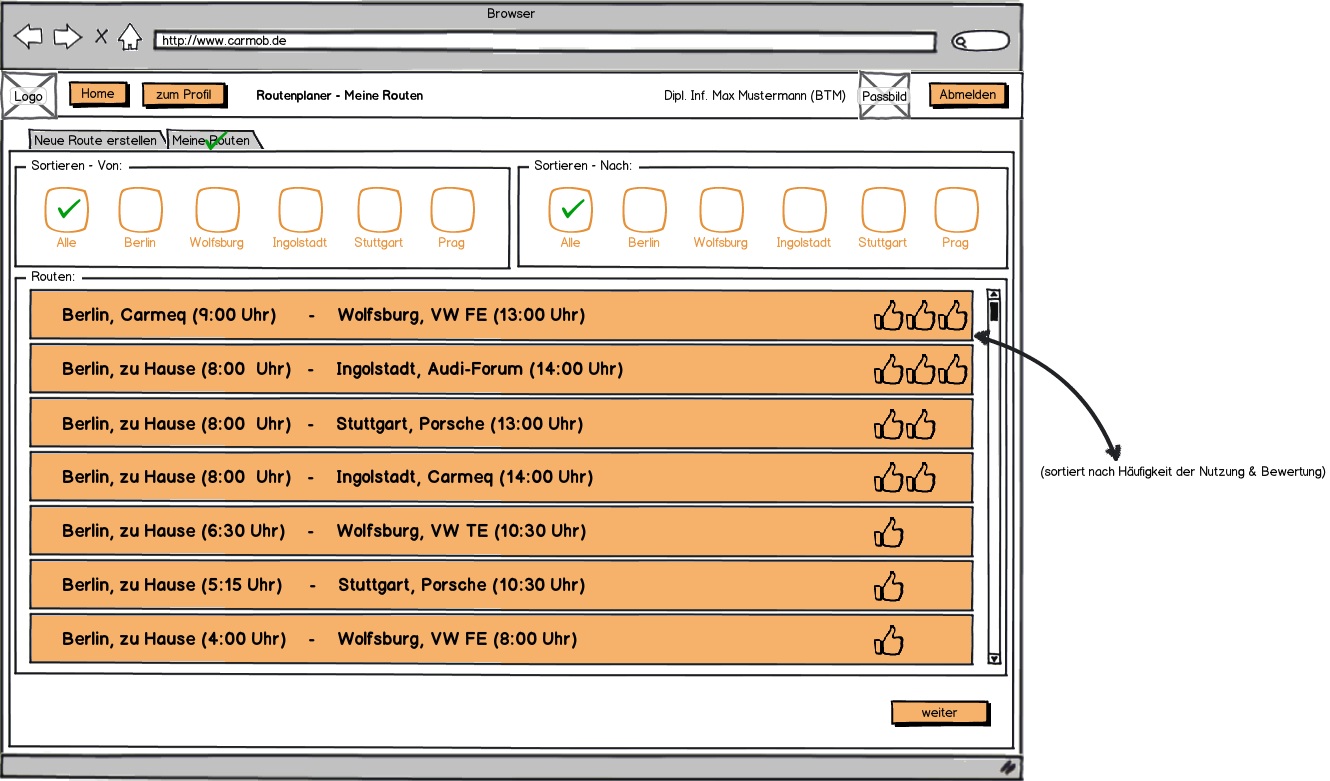
\includegraphics[width=12cm]{10_finaler_paperprototyp_005.png}\\
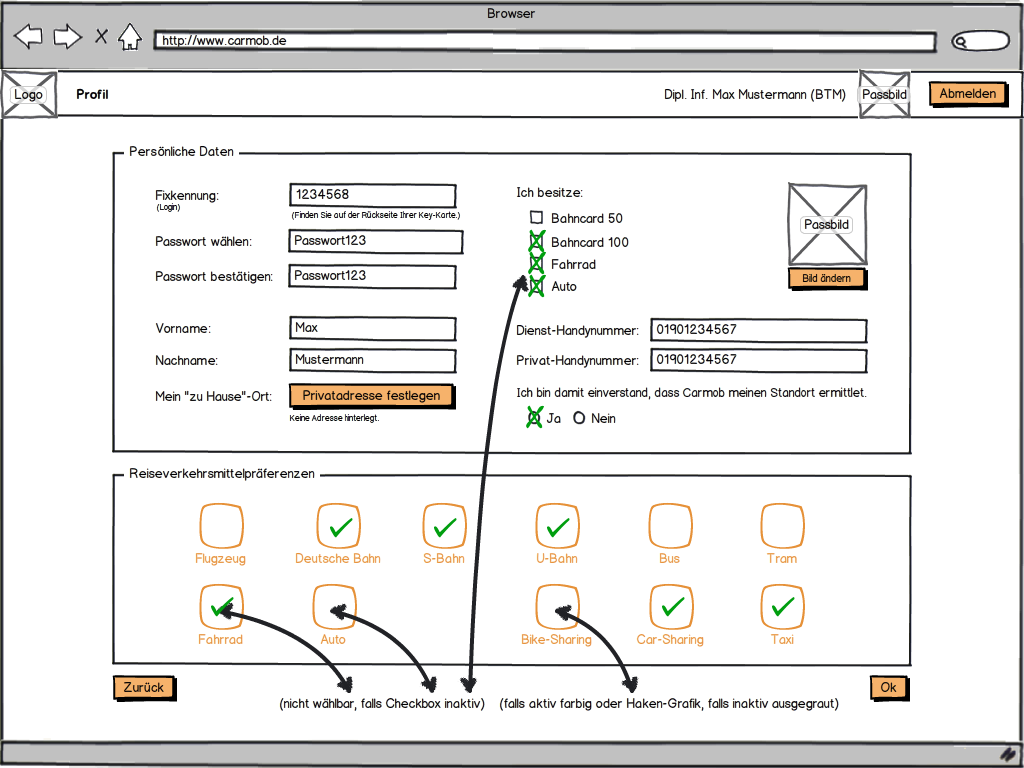
\includegraphics[width=12cm]{10_finaler_paperprototyp_006.png}\\
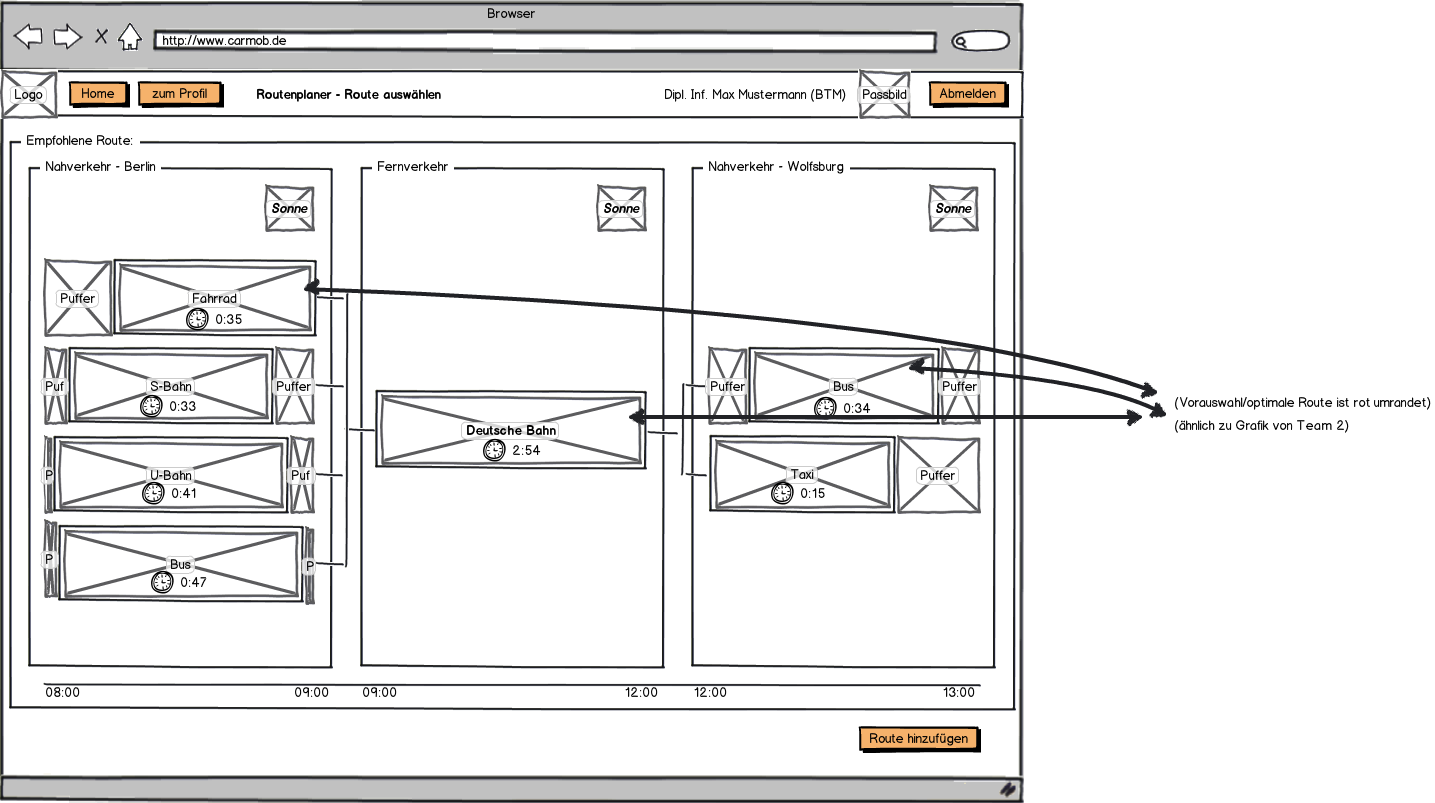
\includegraphics[width=12cm]{10_finaler_paperprototyp_007.png}\\
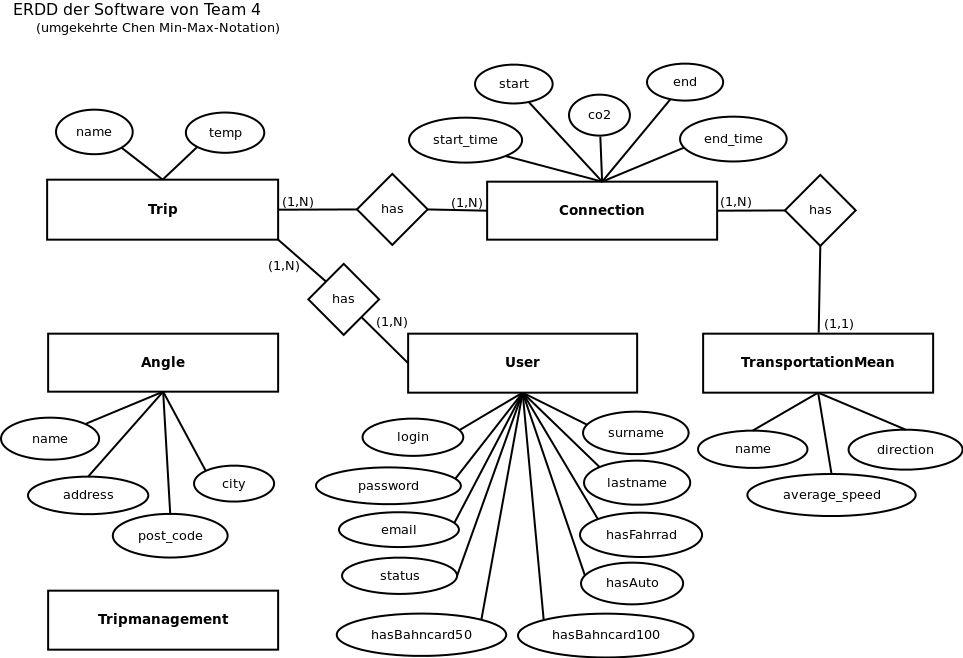
\includegraphics[width=12cm]{11_erdd.png}
\end{center}
\newpage

\section{Phase: 2. Iteration}

In dieser Phase sollte der aktuelle Projektstand mit Mitarbeitern der Carmeq GmbH getestet werden und mit den Erkenntnissen selbst definierte Userstories erstellt und implementiert werden.

\subsection{Woche 07: Routen berechnen}

\subsubsection{Was hat das Team getan?}

Der aktuelle Projektstand wurde von Mitarbeitern der Carmeq GmbH getestet. Wir konnten neben der gew\"ohnlichen Analyse Vorschl\"age zum GUI aufgenommen und im Laufe dieser Phase umgesetzt. Wir haben die HAFAS-API implementiert und funktionierende Adressdaten ermittelt.

\subsubsection{Zentrale Entscheidungen}

Wir haben uns f\"ur die HAFAS-API entschieden, da uns dies vom Kunden empfohlen worden ist.

\subsection{Woche 08: Webservice-GUI}

\subsubsection{Was hat das Team getan?}

Wir haben das noch rudiment\"are GUI anhand der W\"unsche der Mitarbeiter der Carmeq GmbH \"uberarbeitet.

\subsubsection{Zentrale Entscheidungen}

Wir haben uns stark an den W\"unschen der Mitarbeiter der Carmeq GmbH orientiert und die Idee des Human Centered Design ernst genommen.

\subsection{Ergebnisse dieser Phase}

\begin{itemize}
\item Impementierte HAFAS-API (Quellcode)
\item GUI (Quellcode)
\end{itemize}


\section{Phase: 3. Iteration}

In dieser Phase sollte der aktuelle Projektstand mit Mitarbeitern der Carmeq GmbH getestet werden und mit den Erkenntnissen selbst definierte Userstories erstellt und implementiert werden.

\subsection{Woche 09: Nutzerprofil, Deployment, Refactoring}

\subsubsection{Was hat das Team getan?}

Wir haben ein einfaches Nutzerprofil implementiert, die Controller und Views \"uberarbeitet und die Software auf dem Server \texttt{herokuapp.com} deployed.

\subsubsection{Zentrale Entscheidungen}

Wir haben uns dafür entschieden diese Woche für das Refactoring und damit bessere Strukturieren der vorhandenen Software zu investieren, um in den kommenden Wochen schneller voranzukommen.

\subsection{Woche 10: Intermodalit\"at, Mobile-GUI}

\subsubsection{Was hat das Team getan?}

Wir haben den zweiten gro\ss en Teil unserer Software, die mobile Ansicht (OnTheWay-Guide) implementiert und erste intermodale Funktionalit\"at in Form verschiedener Verkehrsmittel hinzugef\"ugt.

\subsubsection{Zentrale Entscheidungen}

Wir haben die mobile Ansicht nah am Paper-Prototyp gestaltet, allerdings direkt Anregungen und Erkenntnisse aus den Tests einflie\ss en lassen.

\subsection{Ergebnisse dieser Phase}

\begin{itemize}
\item Deployment (URL)
\item Mobile-GUI (Quellcode)
\item Intermodalit\"at (Quellcode)
\end{itemize}

\section{Phase: 4. Iteration}

In dieser Phase sollte der aktuelle Projektstand mit Mitarbeitern der Carmeq GmbH getestet werden und mit den Erkenntnissen selbst definierte Userstories erstellt und implementiert werden.

\subsection{Woche 11: Feldtest, GUI, Bedingungsanleitung}

\subsubsection{Was hat das Team getan?}

In dieser Woche haben wir die Software soweit \"uberarbeitet, dass sie in den Feldtest gegeben werden konnte. Wir haben eine kurze Bedienungsanleitung f\"ur die Software geschrieben, damit auch unerfahrene Nutzer eine M\"oglichkeit zur Orientierung haben.

\subsubsection{Zentrale Entscheidungen}

Wir haben uns dazu entschieden die Software auf die wichtigsten Kernfunktionen einzuschr\"anken, um die Akzeptanz beim Nutzer durch das Ausbleiben von Fehler zu erh\"ohen. Wir haben die Bedienungsanleitung direkt in der Software verlinkt, so dass der Nutzer bei auftretenden Fragen immer einen direkten Zugriff auf Erkl\"arungen auch w\"ahrend der Nutzung hat.


\subsection{Woche 12: Schnittstelle, Taxi, CO$_2$}

\subsubsection{Was hat das Team getan?}

Wir haben die Schnittstelle zu Team 1 und einen CO$_2$-Filter implementiert und begonnen ein Marketingkonzept f\"ur die Software zu erstellen.

\subsubsection{Zentrale Entscheidungen}

Wir haben uns als erste Schnittstelle zu den anderen Teams das Team 1 ausgesucht, da wir der Meinung waren, dass, im Verh\"altnis zum Aufwand, der direkte Nutzen f\"ur den Nutzer am gr\"o\ss ten ist. Die CO$_2$-Filterfunktion wurde als besonderer Anreiz f\"ur die Nutzung der Software hinzugef\"ugt. Im Zentrum unseres Marketingkonzepts stehen die Fragen \textit{Was kann der Nutzer mit der Software machen?} und \textit{Welchen Vorteil gewinnt der Nutzer bei der Nutzung unserer Software im direkten Vergleich zur derzeitigen Ist-Situation in der Carmeq GmbH?}

\subsection{Ergebnisse dieser Phase}

\begin{itemize}
\item Schnittstelle zu Team 1 (Quellcode)
\item Bedienungsanleitung (PDF)
\item Verkehrsmittel Taxi (Quellcode)
\item CO$_2$-Berechnung (Quellcode)
\end{itemize}


\includepdf[pages=1-9]{12_bedienungsanleitung.pdf}

\section{Phase: 5. Iteration}

In dieser Phase sollte der aktuelle Projektstand mit Mitarbeitern der Carmeq GmbH getestet werden und mit den Erkenntnissen selbst definierte Userstories erstellt und implementiert werden.\\
Statt einer gew\"ohnlichen Iteration und aufgrund dem immer n\"aher r\"uckenden Ende des Softwareprojekts wurden nur kleine Ausbesserungsarbeiten an der Software vorgenommen und diese in einen pr\"asentierbaren Zustand versetzt.

\subsection{Woche 13: Vorbereitung der Abschlusspr\"asentation}

\subsubsection{Was hat das Team getan?}

In dieser Iteration lag der Fokus des Teams auf der Projektdokumentation, dem abschlie\ss enden Produktdesign und der Gestaltung der Abschlusspr\"asentation.\\
Das Team hat einen Termin f\"ur die Vorbesprechung der Abschlusspr\"asentation mit Fr. Prof. Dr. C. M\"uller-Birn vereinbart und wahrgenommen. Inhalt des Gespr\"achs waren Kritik und Verbesserungsvorschl\"age für den Verlauf und Ablauf der Abschlusspr\"asentation. Wir haben zwei Screencasts f\"ur erstellt.

\subsubsection{Zentrale Entscheidungen}

Der Produktname wird \textit{Twot} lauten. Als Marketingkonzept soll die Persona ihre typischen Probleme w\"ahrend der Planung und Durchf\"uhrung einer typischen Dienstreise durchleben. Somit wird eine ist-Situation geschaffen, die durch unsere Softwarel\"osung als soll-Situation abgel\"ost wird. Die Abschlusspr\"asentation wird zuerst in GoogleDocs erstellt und als PDF exportiert, dann allerdings auf Prezi portiert. Die Prezi-Version wird f\"ur die Abschlusspr\"asentation verwendet. 

\subsection{Ergebnisse dieser Phase}

Wir haben die Projektdokumentation im Quelltext und in Schriftform abgeschlossen. Nach der Erarbeitung eines Marketingkonzepts haben wir die Abschlusspr\"asentation auf verschiedenen Plattformen fertig gestellt.

\begin{itemize}
\item Projektdokumentation (PDF)
\item vollst\"andiges Marketingkonzept (siehe Konzept Abschlusspr\"asentation)
\item Konzept Abschlusspr\"asentation (PDF)
\end{itemize}

\includepdf[pages=1-9]{13_abschlusspraesentation_konzept.pdf}

\section{Phase: Abschlusspr\"asentation}

Diese Phase diente dem Abschluss des Projekts und der Pr\"asentation der Ergebnisse der letzten drei Monate.

\subsection{Woche 14: Abschlusspr\"asentation}

\subsubsection{Was hat das Team getan?}

Wir haben bei der Carmeq GmbH vor breiterem Publikum als gew\"ohnlich unsere Abschlusspr\"asentation gehalten. Nach den Pr\"asentationen haben wir uns von den Mitarbeitern der Carmeq GmbH und den anderen Teams verabschiedet.

\subsubsection{Zentrale Entscheidungen}

Wir haben uns dazu entschieden die Pr\"asentation in drei Teilen zu strukturieren und jeden Teil durch ein anderes Teammitglied pr\"asentieren zu lassen. Zu Beginn haben wir einen \"Uberblick \"uber den bisherigen Projektverlauf im Allgemeinen gegeben. Anschlie\ss end haben wir unsere Persona die typische Problemstellung unseres Softwareprojekts durchleben und unsere L\"osung \textit{Twot} entdecken lassen. Zum Abschluss wurde die Software mit zwei Screencasts, einen f\"ur die Planung und einen f\"ur die Reisebegleitung, vorgestellt.

\subsection{Ergebnisse dieser Phase}

\begin{itemize}
\item Abschlusspr\"asentation (Prezi)
\end{itemize}

\section{Link zu den Repositories}

\subsection{SVN Spline}

Link: \texttt{http://dev.spline.de}

\subsection{GitHub}

Link: \texttt{https://github.com/schmidie/Carmob}

\section{Installationsanleitung (Deployment)}

Die Software wurde auf dem Server herokuapp.com deployed.

\begin{verbatim}
heroku create
git push heroku master
\end{verbatim}

Link: \texttt{http://twot.herokuapp.com}

\end{document}